\newpage\handout[true]
{\textsc{Math 2106-B: Foundations of Mathematical Proof}}{Fall 2025}
{Homework 2 \& 3: Sets}
{\textit{Prof.} \href{https://ceheitsch.github.io/webpage/}{Dr. Christine Heitsch}}{Due Date: September 4th}
{Math 2106-B: HW2}
{\large
  \noindent
  \textbf{Name:} \HandoutAuthor \smallskip \\

  \noindent
  \textbf{GTID:} 903743506 \smallskip \\

  \noindent
  %%% List anyone with whom you discussed the problems
  \textbf{Collaborators:} None. This material reflects independent preparation. \smallskip \\

  \noindent
  %%% List all resources used OTHER than the textbook, lecture notes, 
  %%% webwork problems, ICA questions, and previous homework assignments.
  \textbf{Outside resources:} This work was informed by MATH 2106 course materials 
  (ICAs: in-class activities and WebWork contents) from \HandoutInstitution\ (the course textbook is 
  Chartrand \parencite{chartrand_mathematical_2018}).   
  Outside references specifically include
  textbooks written by 
  Grimaldi \parencite{grimaldi_discrete_2004} (used in MATH 3012) and 
  Rosen \parencite{rosen_discrete_2019} (used in CS 2050). \smallskip \\

  \noindent
  \textbf{Notice}: The answers contain cross-references throughout this document as clickable hyperlinks in most PDF viewers. However, the Gradescope PDF view might not support clickable hyperlinks.
}
\printbibliography[
  heading=bibintoc,   
  title={References}     % change “References” text if needed
]
% `heading=bibnumbered` if you prefer it numbered chapter (in \tableofcontents)
% `heading=bibintoc`    if you prefer it unnumbered but still in the ToC\newpage
The following table presents the standard logical equivalences from these sources together with 
the author's own (or the student, myself, Jaehoon Song) clarifications and labels where applicable.


\begin{table}[h!]
  \centering
  \renewcommand{\arraystretch}{1.2}
  \setlength{\tabcolsep}{8pt}
  \begin{tabular}{|p{5.0cm}|p{5.0cm}|p{5.2cm}|}
    \hline
    \rowcolor[HTML]{E0E0E0}
    \multicolumn{2}{|l|}{\textbf{Logical Equivalences}} & \textbf{Name} \\
    \hline
    $\,p \AND q \equiv q \AND p$ & $\,p \OR q \equiv q \OR p$ & Commutative Law \\
    \hline
    $\, (p \AND q) \AND r \equiv p \AND (q \AND r)$ & $\, (p \OR q) \OR r \equiv p \OR (q \OR r)$ & Associative Law \\
    \hline
    $\,p \AND (q \OR r) \equiv (p \AND q) \OR (p \AND r)$ & $\,p \OR (q \AND r) \equiv (p \OR q) \AND (p \OR r)$ & Distributive Law \\
    \hline
    $\,\overline{p \AND q} \equiv \sNOT{p} \OR \sNOT{q}$ & $\,\overline{p \OR q} \equiv \sNOT{p} \AND \sNOT{q}$ & DeMorgan's Law \\
    \hline
    \multicolumn{2}{|l|}{$\,\overline{\overline{p}} \equiv p$} & Double Negation law \\
    \hline
    $\,p \AND \boldsymbol{T} \equiv p$ & $\,p \OR \boldsymbol{F} \equiv p$ & Identity Law \\
    \hline
    $\,p \OR \boldsymbol{T} \equiv \boldsymbol{T}$ & $\,p \AND \boldsymbol{F} \equiv \boldsymbol{F}$ & Domination Law \\
    \hline
    $\,p \AND p \equiv p$ & $\,p \OR p \equiv p$ & Idempotent Law \\
    \hline
    \multicolumn{2}{|l|}{$\,p \THEN q \equiv \sNOT{p} \OR q$} & Implication Equivalence \\
    \hline
    \multicolumn{2}{|l|}{$\,\overline{p \THEN q} \equiv p \AND \sNOT{q}$} & Negation of Implication \\
    \hline
    \multicolumn{2}{|l|}{$\,p \THEN q \equiv \sNOT{q} \THEN \sNOT{p}$} & Contrapositive Equivalence \\
    \hline
    \multicolumn{2}{|l|}{$\,p \OR \sNOT{p} \equiv \boldsymbol{T}$} & Law of Tautology \\
    \hline
    \multicolumn{2}{|l|}{$\,p \AND \sNOT{p} \equiv \boldsymbol{F}$} & Law of Contradiction \\
    \hline
  \end{tabular}
\end{table}\newpage

The following definitions are presented from standard mathematical sources (\textbf{Sets}).
Clarifications and labels have been added where applicable.

\begin{define}{Basic Set Concepts}\phantomsection\label{def:basic-set-concepts} % \hyperref[def:basic-set-concepts]{YOUR_CONTEXT}
  \begin{enumerate}
    \item \textbf{Universal Set:} A universal set $\setUNIV$ is a
    set that contains all objects under consideration in a particular context or problem.
    \item \textbf{Empty Set:} The empty set, denoted $\setNULL$,
    is the unique set that contains no elements.
    \item \textbf{Subset:} Let $A$ and $B$ be sets. $A$ is a
    subset of $B$ ($A \subseteq B$) if (and only if)
    for all $x \in A$, $x \in B$.
    \item \textbf{Set Equality:} Let $A$ and $B$ be sets. The sets $A$ and $B$ are
    equal ($A = B$) if $A \subseteq B$ and $B \subseteq A$.
    \item \textbf{Power Set:} Let $A$ be a set. The power set of $A$, denoted $\sPOWER{A}$ or $2^A$,
    is the set of all subsets of $A$. That is, $\mathcal{P}(A) = \{S\in\setUNIV : S \subseteq A\}$.
  \end{enumerate}
\end{define}
The following definitions extend the understanding of set operations
and properties.


\begin{define}{Set Operations}\phantomsection\label{def:set-operations} % \hyperref[def:set-operations]{YOUR_CONTEXT}
  \begin{enumerate}
    \item \textbf{Complementary Set:} Let $A$ be a subset of the universal set $\setUNIV$.
    The complement of $A$, denoted $A^c$ or $\overline{A}$, is the set of all elements
    in $\setUNIV$ that are not in $A$. That is, $A^c = \{x \in \setUNIV : x \notin A\}$.
    \item \textbf{Union:} Let $A$ and $B$ be sets. The union of $A$ and $B$,
    denoted $A \cup B$, is the set of all elements that are in $A$, or in $B$, or in both.
    That is, $A \cup B = \{x : x \in A \lor x \in B\}$.
    \item \textbf{Intersection:} Let $A$ and $B$ be sets. The intersection of $A$ and $B$,
    denoted $A \cap B$, is the set of all elements that are in both $A$ and $B$.
    That is, $A \cap B = \{x : x \in A \land x \in B\}$.
    \item \textbf{Set Difference:} Let $A$, $B$ be subsets of a universal set $\setUNIV$.
    The set difference $A \sMINUS B$ is defined to be the set
    $\{ x \in \setUNIV \LDIV x \in A \text{ and } x \notin B\}$. \vspace*{10px}\\
    \textit{It is sometimes called the relative complement of $B$ in $A$,
    and denoted in the textbook as $A - B$.}
    \item \textbf{Cartesian Product:} Let $A$ and $B$ be sets. The Cartesian product of
    $A$ and $B$, denoted $A \sTIMES B$, is the set consisting of all ordered pairs:
    \[
    A \sTIMES B = \{(a, b) \LDIV a \in A, b \in B\}.
    \]
  \end{enumerate}
\end{define}


\newpage

The following claims are given in the reference as well. Let $A,B\in U$, a universal set.


\begin{claim}{Subset of Union: $A \subseteq \sOR{A}{B}$}\phantomsection\label{claim:subset-union} % \hyperref[claim:subset-union]{YOUR_CONTEXT}
  \begin{subprove}[bluecolor]
      Let $x\in U$, assume $x\in A$. Then the statement \inlinequote{$x\in A$ or $x\in B$} is true.
      Hence, by the definition, $\sOR{A}{B}=\{x\in U\LDIV x\in A$ or $x\in B\}$, $x\in \sOR{A}{B}$.
      Thus, $A \subseteq \sOR{A}{B}$.
  \end{subprove}
\end{claim}

\begin{claim}{Empty Subset: $\setNULL \subseteq A$}\phantomsection\label{claim:empty-subset} % \hyperref[claim:empty-subset]{YOUR_CONTEXT}
  \begin{subprove}[bluecolor]
      Let $x\in U$, assume $x\in \setNULL$. But there are no elements in $\setNULL$, so
      $x\in \setNULL$ is false. Since the premise is false, the implication if $x\in \setNULL$,
      then $x\in A$ is true. Thus, $\setNULL \subseteq A$ by definition of \hyperref[def:basic-set-concepts]{subsets}.
  \end{subprove}
\end{claim}

\begin{claim}{Subset as Equality: $\sOR{A}{B}=A$ if and only if $B\subseteq A$}\phantomsection\label{claim:subset-equality} % \hyperref[claim:subset-equality]{YOUR_CONTEXT}
  \begin{subprove}[bluecolor]
      Let $x\in U$, first, we assume $B\subseteq A$, we have already shown
      $A \subseteq \sOR{A}{B}$ by the claim, \hyperref[claim:subset-union]{Subset of Union}. 
      To show $\sOR{A}{B} \subseteq A$, assume $x\in \sOR{A}{B}$.
      By definition, $x\in A$ or $x\in B$. Considering $x\in B$ and assumption
      $B \subseteq A$, $x\in B$ implies $x\in A$. Thus, $\sOR{A}{B} \subseteq A$.
      Hence, if $B\subseteq A$, then $\sOR{A}{B} = A$. \vspace*{10px}\\
      Now, we assume $\sOR{A}{B}=A$. To show $B\subseteq A$, we now assume $x\in B$. Since $x\in B$, by definition
      of union, $x\in \sOR{A}{B} = A$. Therefore, $B\subseteq A$.
  \end{subprove}
\end{claim}


%%%%%%%%%%%%%%%%%%% 9/8/25

Let $\setUNIV$ be a set. 
\begin{claim}{ICA6}\phantomsection\label{claim:ica6} % \hyperref[claim:ica6]{YOUR_CONTEXT}
  For all $A,B\in\setUNIV$, $$A\sTIMES B =\setNULL\THEN \group{A=\setNULL\OR B=\setNULL}$$
  \begin{subprove}[bluecolor]
    Let $A,B\in\setUNIV$. We prove $A\sTIMES B=\setNULL$. Assume it is not the case that 
    $A=\setNULL$ or $B=\setNULL$. Thus, we have $A=\setNULL$ and $B=\setNULL$. 
    Since $A\ne\setNULL$ by assumption, there exists an element $a\in A$. Likewise, there 
    is some $b\in B$ since $B\ne\setNULL$. Thus, $\group{a,b}\in\sBUILD{(x,y)}{x\in A,y\in B}$ 
    by definition. But then, $A\sTIMES B\ne\setNULL$ by definition. Hence, the claim holds. 
  \end{subprove}
\end{claim}


\begin{define}{Relatively Prime Integers (Coprime)}\phantomsection\label{def:relatively-prime} % \hyperref[def:relatively-prime]{YOUR_CONTEXT}
  Let $x,y \in \mathbb{Z}$. The integers $x$ and $y$ are said to be
  \textbf{relatively prime} if and only if
  $\gcd(x,y) = 1$.
\end{define}
\newpage
The following definitions and axioms are presented from standard mathematical sources (\textbf{Number Theory}) together with the author's own (or the student, myself, Jaehoon Song) clarifications and labels where applicable.

\begin{define}{Integers}[def:integers][red]
  $\setZ$: the set of all integers
\end{define}

\begin{define}{Rational Numbers}[def:rational-numbers][red]
  $\setQ$: the set of all rational numbers
\end{define}

\begin{define}{Real Numbers}[def:real-numbers][red]
  $\setR$: the set of all real numbers
\end{define}

\begin{define}{Natural Numbers}[def:natural-numbers][red]
  $\setN$ or $\setZ_{>0}$: the set of all natural numbers which are the set of positive integers (not including $0$)
\end{define}

\begin{define}{Positive Real Numbers}[def:positive-real-numbers][red]
  $\setR_{>0}$: the set of all positive real numbers
\end{define}

\begin{define}{Non-negative Real Numbers}[def:non-negative-real-numbers][red]
  $\setR_{\geq 0}$: the set of all non-negative real numbers
\end{define}


\newpage

The following definitions and claims extend the understanding of integers.

Here are the ICA2 Definitions and Axioms as follows.

\begin{define}{Even Integer}[def:even-integer][red]
  An integer $n$ is \underbar{even} if there exists 
  (existential quantification logic $\exists$) an integer $k$ such that
  \[
  n = 2k.
  \]
\end{define}

\begin{define}{Odd Integer}[def:odd-integer][red]
  An integer $n$ is \underbar{odd} if 
  there exists some integer $k$ such that
  \[
  n = 2k + 1.
  \]
\end{define}

\begin{define}{Closure under Addition}[def:closure-addition][red]
  The sum of two integers is again an 
  integer. (Closure under addition)
\end{define}

\begin{define}{Closure under Multiplication}[def:closure-multiplication][red]
  The product of two integers is again 
  an integer. (Closure under multiplication)
\end{define}

\begin{define}{Odd if and only if Not Even}[def:odd-iff-not-even][red]
  An integer is odd if and only if it 
  is not even.
\end{define}

Here are the ICA3 Definitions and Axioms as follows.

\begin{define}{Universal Closure under Addition}[def:universal-closure-addition][red]
  The sum of two integers (Universal quantification for all, for every, for each) is again an integer. (Closure under addition)
\end{define}

\begin{define}{Universal Closure under Multiplication}[def:universal-closure-multiplication][red]
  The product of two integers (Universal quantification for all, for every, for each) is again an integer. (Closure under multiplication)
\end{define}

\begin{define}{Even Integer Square}[def:even-integer-square][red]
  An integer $n$ is even if and only if $n^2$ is even.
\end{define}

\newpage

The following claims are given in the reference as well.

\begin{define}{Sum of Even Integers}[claim:sum-even-integers][red]
  The sum of two even integers is again an even integer.
  \begin{subprove}[red]
    Let $x$ be an integer and $y$ be an integer ($\forall x,y \in \setZ$). 
    Suppose $x$ is even and $y$ is even. Then, by \nameref{def:even-integer}, there exists an integer 
    $k$ and an integer $j$ such that $x=2k$ and $y=2j$. Then, 
    $x+y=\left(2k\right)+\left(2j\right)=2\left(k+j\right)$. By \nameref{def:closure-addition}, since $k$ and 
    $j$ are integers, then so is $\left(k+j\right)$. Hence, by definition, $x+y$ is an 
    even integer.
  \end{subprove}
\end{define}

The following definitions extend the understanding of integers including divisibility.

\begin{define}{Divisibility}[def:divisibility][red]
  An integer $n$ divides an integer $m$, denoted $n \LDIV m$, if there 
  exists an integer $k$ such that $m=n k$. Otherwise, $n \nmid m$.
\end{define}

The following definitions extend the classification of real numbers into rational and irrational numbers.

\begin{define}{Rational Number}[def:rational-number][red]
  A real number $x$ is \underbar{rational} if there exist integers $a$ and $b$ with $b \neq 0$ such that $bx = a$.
  Otherwise, $x$ is \underbar{irrational}.

  \textbf{Note}: Compare the rational number definition with the even/odd axiom \inlinequote{odd iff not even} from \nameref{def:odd-iff-not-even}.
\end{define}

The following claims are given in the reference as well.

\begin{define}{Irrationality of $\sqrt{2}$}[claim:sqrt2-irrational][red]
  $\sqrt{2}$ is irrational.
  \begin{subprove}[red]
    Suppose $\sqrt{2}$ is rational. Then, by \nameref{def:rational-number}, there exists $a,b\in \setZ$ 
    with $b\ne 0$ such that $b\cdot\sqrt{2}=a$. We may further assume that any factors 
    common to $a$ and $b$ have already been removed.\\

    Then, squaring both sides, this yields $2\cdot b^2 = a^2$.
    Since products of integers are again integers by \nameref{def:closure-multiplication}, we have that $a^2,b^2\in \setZ$.
    Thus, by definition, $a^2$ is even. Therefore, by \nameref{def:even-integer-square}, $a$ is even. 
    Thus, there exists $c\in\setZ$ such that $a=2c$. Then
    $$
    2b^2=a^2={2c}^2=4c^2
    $$
    Then, $b^2=2c^2$. Then, as before, $b^2$ is even, so $b$ is even.
    However, $a$ and $b$ both being even contradicts the fact that any factors 
    common to $a$ and $b$ have already been removed.
  \end{subprove}
\end{define}






%%%%%%%%%%%%%%%%%%% New style (refactor model)
\begin{define}{Relatively Prime Integers (Coprime)}[def:relatively-prime][red]
  Let $x,y \in \mathbb{Z}$. The integers $x$ and $y$ are said to be
  \textbf{relatively prime} if and only if
  $\gcd(x,y) = 1$.
\end{define}\newpage




%%%%%%%%%%%%%%%%%%%%%%%%%%%%%%%%%%%%%%%%%%%%%%%%%%%%%%%%%%%%%%%%%%%%%%%
% References
%%%%%%%%%%%%%%%%%%%%%%%%%%%%%%%%%%%%%%%%%%%%%%%%%%%%%%%%%%%%%%%%%%%%%%%

\begin{define}{Complementary Set}[def:complementary-set][red]
  Let $A$ be a subset of the universal set $\setUNIV$. The complement of $A$, 
  denoted $A^c$ or $\sNOT{A}$, is the set of all elements in $\setUNIV$ that are not in $A$. 
  That is, $\sNOT{A} = \{x \in \setUNIV : x \notin A\}$.
\end{define}


\begin{define}{Set Equality}[def:set-equality][red]
  Let $A$ and $B$ be sets. The sets $A$ and $B$ are equal ($A = B$) iff $A \subseteq B$ and $B \subseteq A$.
  \end{define}
  \begin{define}{Subset}[def:subset][red]
    Let $A$ and $B$ be sets. $A$ is a subset of $B$ ($A \subseteq B$) if (and only if) for all $x \in A$, then $x \in B$.
  \end{define}
  \begin{define}{Set Intersection}[def:set-intersection][red]
    Let $A$ and $B$ be sets. The intersection of $A$ and $B$, denoted $A \sAND B$, is the 
    set of all elements that are in both $A$ and $B$. That is, $A \sAND B = \{x : x \in A \text{ and } x \in B\}$.
  \end{define}




%%%%%%%%%%%%%%%%%%%%%%%%%%%%%%%%%%%%%%%%%%%%%%%%%%%%%%%%%%%%%%%%%%%%%%%
% Problems
%%%%%%%%%%%%%%%%%%%%%%%%%%%%%%%%%%%%%%%%%%%%%%%%%%%%%%%%%%%%%%%%%%%%%%%
\newpage
\begin{enumerate} 
  \item Let $a \in \setZ$. Prove that $3\LDIV a^2$ if and only if $3\LDIV a$.
  \label{prob:divisibility-by-3} % Problem~\ref{prob:divisibility-by-3}
  \textit{You may use the fact that every integer can be written as 
  exactly one of $3k$, $3k + 1$, or $3k+2$ for some integer $k$.}
  \begin{subprove}
    Let $a \in \setZ$ be arbitrary. \vspace*{10px}\\
    ($\Rightarrow$) The contrapositive of the given statement is \inlinequote{$3\NDIV a$ only if $3\NDIV a^2$.}
    Assume $3\NDIV a$ for the sake of contrapositive proof. 
    By the given fact, $a$ can be written as exactly one of $3k + 1$ or $3k+2$ for some 
    integer $k$ since $a$ cannot be multiple of $3$.
    \begin{itemize}
      \item If $a = 3k + 1$, then $a^2 = (3k + 1)^2 = 9k^2 + 6k + 1 = 3(3k^2 + 2k) + 1$. 
      Since $3k^2 + 2k$ is also an integer by Closure Property of Integers, by definition of 
      divisibility, $3\NDIV a^2$.
      \item If $a = 3k + 2$, then $a^2 = (3k + 2)^2 = 9k^2 + 12k + 4 = 3(3k^2 + 4k + 1) + 1$. 
      Since $3k^2 + 4k + 1$ is also an integer by Closure Property of Integers, by definition of 
      divisibility, $3\NDIV a^2$.
    \end{itemize}
    In both cases, $3\NDIV a^2$.
    Therefore, by contrapositive, $3\LDIV a^2$ only if $3\LDIV a$.\vspace*{10px}\\
    ($\Leftarrow$) Assume $3\LDIV a$ for the sake of direct proof. 
    Since $3\LDIV a$, there exists an integer $k$ such that $a = 3k$ by definition of divisibility.
    Then $a^2 = (3k)^2 = 9k^2 = 3(3k^2)$.
    Since $3k^2$ is also an integer by Closure Property of Integers, by definition of divisibility, $3\LDIV a^2$.
    Thus, $3\LDIV a^2$ if $3\LDIV a$.\vspace*{10px}\\
    Therefore, by ($\Rightarrow$) and ($\Leftarrow$), $3\LDIV a^2$ if and only if $3\LDIV a$.
  \end{subprove}
  
  \item It is to be proven that $\sqrt{3}$ is irrational.
  \label{prob:sqrt3-irrational} % Problem~\ref{prob:sqrt3-irrational}
  \textit{Hint: The result from Problem~\ref{prob:divisibility-by-3} should be used.}
  \begin{subprove}
    Suppose $\sqrt{3}$ is rational for the sake of contradiction. By the definition of 
    a rational number, there exist integers $p$ and $q$, with $q \neq 0$, such that 
    $$\sqrt{3} = \frac{p}{q}.$$ 
    It is further assumed that the fraction $\frac{p}{q}$ has 
    been reduced to its lowest terms, meaning that $p$ and $q$ are relatively prime, 
    i.e., $\gcd(p,q) = 1$. Then, the equation will be rearranged as follows.
    $$p^2 = 3q^2.$$
    Since $q$ is an integer, $q^2$ is an integer by Closure Property of 
    Integers, which implies $3\LDIV p^2$ and $3\LDIV p$ by Problem~\ref{prob:divisibility-by-3}.
    Furthermore, by the definition of divisibility, there exists an integer $k$ such that $p = 3k$. 
    Thus,
    $$
    p^2 =(3k)^2 = 9k^2 = 3q^2.
    $$
    Moreover,
    $$
    3k^2 = q^2
    $$
    which implies again $3\LDIV q^2$ and $3\LDIV q$ by Problem~\ref{prob:divisibility-by-3}.
    This means that $p$ and $q$ share a common factor of $3$, which contradicts the assumption 
    that $\gcd(p,q) = 1$ (or $p$ and $q$ are relatively prime.) 
    Therefore, $\sqrt{3}$ is irrational.
  \end{subprove}
  \newpage


  \item Prove the following directly from the definition.   \\
  Let $a$, $b$, $c$, $d$, $x$ and $y$ be integers with $a \neq 0$ and $b \neq 0$.
  \begin{enumerate}
    \item If $a\LDIV c$ and $b\LDIV d$, then $ab\LDIV cd$.
    \begin{subprove}
      Assume $a\LDIV c$ and $b\LDIV d$ for the sake of direct proof.
      By definition of divisibility, there exist integers $k$ and $l$ such that $c = ak$ and $d = bl$.
      Then, $cd = (ak)(bl) = (ab)(kl)$. Since $kl$ is also an integer, by Closure Property 
      of Integers and definition of divisibility, $ab\LDIV cd$.
    \end{subprove}
    
    \item If $a\LDIV c$ and $a\LDIV d$, then $a\LDIV cx + dy$.
    \begin{subprove}
      Assume $a\LDIV c$ and $a\LDIV d$ for the sake of direct proof.
      By definition of divisibility, there exist integers $k$ and $l$ such that $c = ak$ and $d = al$.
      Then $cx + dy = (ak)x + (al)y = a(kx + ly)$.
      Since $kx + ly$ is an integer, by Closure Property 
      of Integers and definition of divisibility, $a\LDIV cx + dy$.
    \end{subprove}
    
    \item If $a\LDIV b$ and $b\LDIV a$, then $a = b$ or $a = -b$.
    \begin{subprove}
      Assume $a\LDIV b$ and $b\LDIV a$ for the sake of direct proof.
      By definition of divisibility, there exist integers $k$ and $l$ such that $b = ak$ and $a = bl$. 
      Without loss of generality of arguing $a$ and $b$ seperately, $b = (bl)k = b(lk)$ by substitution.
      Since $b \neq 0$ (and $a \neq 0$ as well) by condition, $1 = lk$ by dividing $b$ on both sides. The only integer solutions 
      to this equation are $(l,k) = (1,1)$ or $(l,k) = (-1,-1)$.
      If $(l,k) = (1,1)$, then $a = b$.
      If $(l,k) = (-1,-1)$, then $a = -b$.
      Therefore, $a = b$ or $a = -b$.
    \end{subprove}
    
    \item If $a\NDIV cd$, then $a\NDIV c$ and $a\NDIV d$.
    \begin{subprove}
      The contrapositive of the given statement is \inlinequote{if $a\LDIV c$ or $a\LDIV d$, then $a\LDIV cd$.}
      Assume $a\LDIV c$ or $a\LDIV d$ for the sake of direct contrapositive.
      \begin{itemize}
        \item If $a\LDIV c$, then there exists an integer $k$ such that $c = ak$. 
        Then $cd = (ak)d = a(kd)$. Since $kd$ is also an integer, $a\LDIV cd$.
        \item If $a\LDIV d$, then there exists an integer $l$ such that $d = al$. 
        Then $cd = c(al) = a(cl)$. Since $cl$ is also an integer, $a\LDIV cd$.
      \end{itemize}
      In both cases, $a\LDIV cd$. Therefore, by contrapositive, 
      if $a\NDIV cd$, then $a\NDIV c$ and $a\NDIV d$.
    \end{subprove}
  \end{enumerate}

  \newpage


  \item Let $A$, $B$ be subsets of a universal set $\setUNIV$.
  Prove the following using the element method:
  \begin{enumerate}
    \item $A \sMINUS B \subseteq A$.
    \begin{subprove}
      Let $x \in A \sMINUS B$ be arbitrary, for the sake of direct proof.
      By definition of set difference, $x \in A$ and $x \notin B$. Thus, $x \in A$ (trivial).
      Therefore, $A \sMINUS B \subseteq A$ by definition of Subset.
    \end{subprove}
    
    \item $A \sMINUS B = A \sAND \sNOT{B}$
    \begin{subprove}
      By definition, the equality $A \sMINUS B = A \sAND \sNOT{B}$ 
      requires showing both directions of subset relations, 
      $A \sMINUS B \subseteq A \sAND \sNOT{B}$ and 
      $A \sMINUS B \supseteq A \sAND \sNOT{B}$.\vspace*{10px}\\
      ($\subseteq$) Let $x \in A \sMINUS B$ be arbitrary.
      By definition of set difference, $x \in A$ and $x \notin B$.
      Since $x \notin B$ by definition of complementary set, it follows that $x \in \sNOT{B}$.
      Therefore, $x \in A$ and $x \in \sNOT{B}$, so $x \in A \sAND \sNOT{B}$.
      Hence, $A \sMINUS B \subseteq A \sAND \sNOT{B}$.\vspace*{10px}\\
      ($\supseteq$) Let $x \in A \sAND \sNOT{B}$ be arbitrary.
      By definition of intersection, $x \in A$ and $x \in \sNOT{B}$.
      Since $x \in \sNOT{B}$, it follows that $x \notin B$ by definition of complementary set.
      Therefore, $x \in A$ and $x \notin B$, so $x \in A \sMINUS B$.
      Hence, $A \sAND \sNOT{B} \subseteq A \sMINUS B$.\vspace*{10px}\\
      Therefore, by ($\subseteq$) and ($\supseteq$), $A \sMINUS B = A \sAND \sNOT{B}$.
    \end{subprove}
    
    \item $A \sAND (B \sMINUS A) = \setNULL$.
    \begin{subprove}
      Assume there exists an element $x \in A \sAND (B \sMINUS A)$ by negation of empty set definition for 
      the sake of contradiction. Then $x \in A$ and $x \in B \sMINUS A$.
      Since $x \in B \sMINUS A$, it follows that $x \in B$ and $x \notin A$, 
      which contradicts the assumption, $x \in A$.
      Therefore, $A \sAND (B \sMINUS A) = \setNULL$.
    \end{subprove}
    
    \item $A \sOR (B \sMINUS A) = A \sOR B$.
    \begin{subprove}
      By definition, the equality $A \sOR (B \sMINUS A) = A \sOR B$ 
      requires showing both directions of subset relations, 
      $A \sOR (B \sMINUS A) \subseteq A \sOR B$ and 
      $A \sOR (B \sMINUS A) \supseteq A \sOR B$.\vspace*{10px}\\
      ($\subseteq$) Let $x \in A \sOR (B \sMINUS A)$ be arbitrary.
      Then $x \in A$ or $x \in B \sMINUS A$.
      If $x \in A$, then $x \in A \sOR B$ as well (trivially).
      If $x \in B \sMINUS A$, then $x \in B$ and $x \notin A$, so $x \in B$, 
      which also (trivially) implies $x \in A \sOR B$.
      In both cases, $x \in A \sOR B$. Hence, $A \sOR (B \sMINUS A) \subseteq A \sOR B$.\vspace*{10px}\\
      ($\supseteq$) Let $x \in A \sOR B$ be arbitrary.
      Then $x \in A$ or $x \in B$. If $x \in A$, then $x \in A \sOR (B \sMINUS A)$ as well (trivially). 
      Next, if $x \in B$, then either $x \in A$ or $x \notin A$.
      \begin{itemize}
        \item If $x \in A$, then $x \in A \sOR (B \sMINUS A)$. (trivial)
        \item If $x \notin A$, then $x \in B \sMINUS A$ by definition of set 
        difference, so $x \in A \sOR (B \sMINUS A)$. (trivial)
      \end{itemize}
      In all cases, $x \in A \sOR (B \sMINUS A)$. Hence, $A \sOR B \subseteq A \sOR (B \sMINUS A)$.\vspace*{10px}\\
      Therefore, by ($\subseteq$) and ($\supseteq$), $A \sOR (B \sMINUS A) = A \sOR B$.
    \end{subprove}
  \end{enumerate}

  \newpage


  \item Let $A$, $B$, and $C$ be subsets of a universal set $\setUNIV$.
  Prove or disprove: 
  \begin{enumerate}
    \item If \(A \sAND B = A \sAND C\), then \(B = C\).
    \begin{subdisprove}
      Let $\setUNIV = \{1, 2, 3, 4\}$, $A = \{1, 2\}$, 
      $B = \{1, 3\}$, and $C = \{1, 4\}$ be subsets of a universal set $\setUNIV$
      for the sake of counterexample.
      Then, $A \sAND B = \{1\}$ and $A \sAND C = \{1\}$, that is, $A \sAND B = A \sAND C$.
      However, $B = \{1, 3\} \neq \{1, 4\} = C$. Therefore, it is \textbf{false} 
      that \(A \sAND B = A \sAND C\) only if \(B = C\).
    \end{subdisprove}
    
    \item If \(A \sOR B = A \sOR C\), then \(B = C\).
    \begin{subdisprove}
      Let $\setUNIV = \{1, 2, 3, 4\}$, $A = \{1, 2\}$, $B = \{2, 3\}$, and $C = \{3\}$ 
      be subsets of a universal set $\setUNIV$
      for the sake of counterexample.
      Then $A \sOR B = \{1, 2, 3\}$ and $A \sOR C = \{1, 2, 3\}$, so $A \sOR B = A \sOR C$.
      However, $B = \{2, 3\} \neq \{3\} = C$.
      Therefore, it is \textbf{false} that \(A \sOR B = A \sOR C\) only if \(B = C\).
    \end{subdisprove}
    
    \item If \(A \sAND B = A \sAND C\) and \(A \sOR B = A \sOR C\), then \(B = C\).
    \begin{subprove}
      Assume $A \sAND B = A \sAND C$ and $A \sOR B = A \sOR C$ for 
      the sake of direct proof.
      By definition of set equality, both directions of subset relations are 
      required as follows.\vspace*{10px}\\
      ($\subseteq$) Let $x \in B$ be arbitrary.
      Since $x \in B$, it follows that $x \in A \sOR B = A \sOR C$.
      Therefore, $x \in A$ or $x \in C$ (trivial). If $x \in A$, then 
      $x \in A \sAND B = A \sAND C$, so $x \in C$.
      Hence, $B \subseteq C$.\vspace*{10px}\\
      ($\supseteq$) Let $x \in C$ be arbitrary.
      Since $x \in C$, it follows that $x \in A \sOR C = A \sOR B$.
      Therefore, $x \in A$ or $x \in B$ (trivial).
      If $x \in A$, then $x \in A \sAND C = A \sAND B$, so $x \in B$.
      Hence, $C \subseteq B$.\vspace*{10px}\\
      Therefore, by ($\subseteq$) and ($\supseteq$), \(B = C\) when \(A \sAND B = A \sAND C\) and \(A \sOR B = A \sOR C\).
    \end{subprove}
  \end{enumerate}

  \newpage


  \item Let $A$, $B$ be subsets of a universal set $\setUNIV$.
  Prove or disprove:
  \begin{enumerate}
    \item $A \sTIMES B = \setNULL$ if $A = \setNULL$ or $B = \setNULL$.
    \begin{subprove}
      Assume $A = \setNULL$ or $B = \setNULL$ for the sake of direct proof.
      If $A = \setNULL$, then $A \sTIMES B = \setNULL \sTIMES B = \setNULL$ (since there are no first coordinate value, meaning there are no coordinates).
      If $B = \setNULL$, then $A \sTIMES B = A \sTIMES \setNULL = \setNULL$ (since there are no second coordinate value, meaning there are no coordinates).
      Therefore, direct proof by cases, if $A = \setNULL$ or $B = \setNULL$, then $A \sTIMES B = \setNULL$.
    \end{subprove}
    
    \item $A \sTIMES B = \setNULL$ only if $A = \setNULL$ or $B = \setNULL$.
    \begin{subprove}
      The contrapositive of the given statement is \inlinequote{if $A \neq \setNULL$ 
      and $B \neq \setNULL$, then $A \sTIMES B \neq \setNULL$.}
      Assume $A \neq \setNULL$ and $B \neq \setNULL$.
      Since $A \neq \setNULL$, there exists an element $a \in A$.
      Without loss of generality, there exists an element $b \in B$.
      Then $(a,b) \in A \sTIMES B$ by definition of Cartesian product.
      Therefore, $A \sTIMES B \neq \setNULL$ since there exists an element.
      Therefore, by contrapositive, if $A \sTIMES B = \setNULL$, then $A = \setNULL$ or $B = \setNULL$.
    \end{subprove}
  \end{enumerate}

\end{enumerate}
















%%%%%%%%%%%%%%%%%%%%%%%%%%%%%%%%%%%%%%%%%%%%%%%%%%%%%%%%%%%%%%%%%%%%%%%
% Problems
%%%%%%%%%%%%%%%%%%%%%%%%%%%%%%%%%%%%%%%%%%%%%%%%%%%%%%%%%%%%%%%%%%%%%%%
\newpage
\begin{enumerate} 
  \newpage
  \item Let $A$, $B$, $C$, and $D$ be subsets of a universal set $\setUNIV$. 
  Prove the following propositions.
  \textit{This proves that the three subsets are a partition of 
  $(A \sOR B)$. Partitions will be very important to 
  understanding equivalence relations.}
  \begin{enumerate}
    \item $(A \sOR B)=(A \sAND B) \sOR(A \sMINUS B) \sOR(B \sMINUS A)$.\label{prob:partite-a}
    \begin{define}{Set Difference}[def:set-difference][red]
      Let $A$, $B$ be subsets of a universal set $\setUNIV$. The set difference $A \sMINUS B$ is defined to be the set $\{ x \in \setUNIV \LDIV x \in A \text{ and } x \notin B\}$. \vspace*{5px}\\
      \textit{It is sometimes called the relative complement of $B$ in $A$, and denoted in the textbook as $A - B$.}
    \end{define}
    \begin{subprove}
      By definition of \nameref{def:set-equality}, $(A \sOR B)=(A \sAND B) \sOR(A \sMINUS B) \sOR(B \sMINUS A)$ 
      requires showing both directions of \nameref{def:subset}s, as follows.\vspace*{5px}\\
      ($\subseteq$) Let $x \in A \sOR B$ be arbitrary. Then, $x \in A$ or $x \in B$ 
      by definition of \nameref{def:set-union}. Consider the following cases.
      \begin{itemize}
        \item If $x \in A$ and $x \in B$, then $x \in A \sAND B$ by definition of \nameref{def:set-intersection}.
        \item If $x \in A$ and $x \notin B$, then $x \in A \sMINUS B$ by definition of \nameref{def:set-difference}.
        \item If $x \notin A$ and $x \in B$, then $x \in B \sMINUS A$ by definition.
      \end{itemize}
      In all cases, $x \in (A \sAND B) \sOR(A \sMINUS B) \sOR(B \sMINUS A)$. 
      Hence, proof by cases, $(A \sOR B) \subseteq (A \sAND B) \sOR(A \sMINUS B) \sOR(B \sMINUS A)$.\vspace*{5px}\\
      ($\supseteq$) Let $x \in (A \sAND B) \sOR(A \sMINUS B) \sOR(B \sMINUS A)$ be arbitrary. 
      Then, $x \in A \sAND B$ or $x \in A \sMINUS B$ or $x \in B \sMINUS A$. Consider the following cases.
      \begin{itemize}
        \item If $x \in A \sAND B$, then $x \in A$ and $x \in B$ by definition, so $x \in A \sOR B$.
        \item If $x \in A \sMINUS B$, then $x \in A$ by definition, so $x \in A \sOR B$ by definition.
        \item If $x \in B \sMINUS A$, then $x \in B$ by definition, so $x \in A \sOR B$ by definition.
      \end{itemize}
      Hence, proof by cases, $(A \sAND B) \sOR(A \sMINUS B) \sOR(B \sMINUS A) \subseteq A \sOR B$.\vspace*{5px}\\
      Therefore, by ($\subseteq$) and ($\supseteq$), 
      $(A \sOR B)=(A \sAND B) \sOR(A \sMINUS B) \sOR(B \sMINUS A)$.
    \end{subprove}

    \item $(A \sAND B)$, $(A \sMINUS B)$, and $(B \sMINUS A)$ are all pairwise disjoint. \label{prob:partite-b}
    \begin{define}{Pairwise Disjoint Sets}[def:pairwise-disjoint][red]
      Let $A_1, A_2, \ldots, A_n$ be sets. The collection $\{A_1, A_2, \ldots, A_n\}$ 
      is \textbf{pairwise disjoint} if and only if
      \[
        \forall\, i, j \in \{1, \ldots, n\},\; i \neq j \THEN A_i \cap A_j = \emptyset.
      \]
    \end{define}
    \begin{subprove}
      It is required to show that any two of these sets have empty intersection,
      \begin{itemize}
        \item To claim $(A \sAND B) \sAND (A \sMINUS B) = \setNULL$,
        assume there exists $x \in (A \sAND B) \sAND (A \sMINUS B)$ for 
        the sake of contradiction. Then, $x \in A \sAND B$ and $x \in A \sMINUS B$. 
        Since $x \in A \sAND B$, it follows that $x \in A$ and $x \in B$ by definition of \nameref{def:set-intersection}. 
        Since $x \in A \sMINUS B$, it follows that $x \in A$ and $x \notin B$ by definition of \nameref{def:set-difference}, 
        which contradicts $x \in B$. Therefore, $(A \sAND B) \sAND (A \sMINUS B) = \setNULL$.
        \item To claim $(A \sAND B) \sAND (B \sMINUS A) = \setNULL$, without loss of generality, 
        it is symmetrical to the previous case, with the roles of sets $A$ and $B$ swapped.
        Hence, trivially, $(A \sAND B) \sAND (B \sMINUS A) = \setNULL$.
        \item To claim $(A \sMINUS B) \sAND (B \sMINUS A) = \setNULL$,
        assume there exists $x \in (A \sMINUS B) \sAND (B \sMINUS A)$ for 
        the sake of contradiction. Then, $x \in A \sMINUS B$ and $x \in B \sMINUS A$. 
        Since $x \in A \sMINUS B$, it follows that $x \in A$ and $x \notin B$ by definition of \nameref{def:set-difference}. 
        Since $x \in B \sMINUS A$, it follows that $x \in B$ and $x \notin A$ by definition of \nameref{def:set-difference}, 
        which contradicts both $x \notin B$ and $x \in A$ at the same time. 
        Therefore, $(A \sMINUS B) \sAND (B \sMINUS A) = \setNULL$.
      \end{itemize}
      Therefore, $(A \sAND B)$, $(A \sMINUS B)$, and $(B \sMINUS A)$ are all pairwise disjoint by definition of \nameref{def:pairwise-disjoint}.
    \end{subprove}


    \item $(A \sAND B)$, $(A \sMINUS B)$, and $(B \sMINUS A)$ are partition.
    \begin{define}{Partition}[def:partition][red]
      Let $A$ be a nonempty set. A collection $\mathcal{P}$ of subsets of $A$ is defined as a \emph{partition} of $A$ if and only if the following conditions hold:
      \begin{itemize}
        \item[\textbf{1.}] \textbf{Non-emptiness:} No set in the collection is empty.
          $$ \forall S \in \mathcal{P}, \; S \neq \emptyset $$
        \item[\textbf{2.}] \textbf{Pairwise Disjointness:} The intersection of any two distinct sets in the collection is the empty set.
          $$ \forall S_1, S_2 \in \mathcal{P}, \; S_1 \neq S_2 \THEN S_1 \cap S_2 = \emptyset $$
        \item[\textbf{3.}] \textbf{Union:} The union of all sets in the collection constitutes the entire set $A$.
          $$ \bigcup_{S \in \mathcal{P}} S = A $$
      \end{itemize}
      The elements of $\mathcal{P}$ are referred to as the blocks or cells of the partition.
    \end{define}
    \begin{subprove}
      By the problems \ref{prob:partite-a}, \ref{prob:partite-b}, and \nameref{def:partition}, 
      $\set{(A \sAND B),\ (A \sMINUS B),\ (B \sMINUS A)}$ is a partition of $A$.
    \end{subprove}



  \end{enumerate}
  




  \newpage
  \item Let $A$, $B$, $C$, and $D$ be subsets of a universal set $\setUNIV$. 
  Prove or disprove the following propositions.\\
  \textit{Likewise, Cartesian product of sets (above) and the power set of a set (below) will be very important in the next part of the course.}
  \begin{enumerate}
    \item $(A \sTIMES B) \sAND(C \sTIMES D) \subseteq(A \sAND C) \sTIMES(B \sAND D)$.
    \begin{define}{Cartesian Product}[def:cartesian-product][red]
      Let $A$ and $B$ be sets. The Cartesian product of $A$ and $B$, denoted $A \sTIMES B$, is the set consisting of all ordered pairs:
      \[
      A \sTIMES B = \{(a, b) \LDIV a \in A, b \in B\}.
      \]
    \end{define}
    \begin{subprove}
      Let $(x,y) \in (A \sTIMES B) \sAND(C \sTIMES D)$ be arbitrary for the sake of directly showing ($\subseteq$). 
      Then, $(x,y) \in A \sTIMES B$ and $(x,y) \in C \sTIMES D$. 
      Since $(x,y) \in A \sTIMES B$, it follows that $x \in A$ 
      and $y \in B$ by definition of \nameref{def:cartesian-product}. Since $(x,y) \in C \sTIMES D$, it follows 
      that $x \in C$ and $y \in D$ as well.
      Thus, $x \in A \sAND C$ 
      and $y \in B \sAND D$ by definition of \nameref{def:set-intersection}, 
      so $(x,y) \in (A \sAND C) \sTIMES(B \sAND D)$.
      Hence, $(A \sTIMES B) \sAND(C \sTIMES D) \subseteq(A \sAND C) \sTIMES(B \sAND D)$.
    \end{subprove}

    \item $(A \sAND C) \sTIMES(B \sAND D) \subseteq(A \sTIMES B) \sAND(C \sTIMES D)$.
    \begin{subprove}
      Let $(x,y) \in (A \sAND C) \sTIMES(B \sAND D)$ be arbitrary for the sake of directly showing ($\subseteq$). 
      Then, $x \in A \sAND C$ and $y \in B \sAND D$ by definition of \nameref{def:cartesian-product}. 
      Since $x \in A \sAND C$, it follows that $x \in A$ and $x \in C$ by definition of \nameref{def:set-intersection}. 
      Since $y \in B \sAND D$, it follows that $y \in B$ and $y \in D$.
      Therefore, $(x,y) \in A \sTIMES B$ and $(x,y) \in C \sTIMES D$ since logical AND (\AND) is commutative.
      Thus, $(x,y) \in (A \sTIMES B) \sAND(C \sTIMES D)$.
      Hence, $(A \sAND C) \sTIMES(B \sAND D) \subseteq(A \sTIMES B) \sAND(C \sTIMES D)$.
    \end{subprove}

    \item $(A \sTIMES B) \sOR(C \sTIMES D) \subseteq(A \sOR C) \sTIMES(B \sOR D)$.
    \begin{subprove}
      Let $(x,y) \in (A \sTIMES B) \sOR(C \sTIMES D)$ be arbitrary for the sake of directly showing ($\subseteq$). 
      Then, $(x,y) \in A \sTIMES B$ or $(x,y) \in C \sTIMES D$ by definition of \nameref{def:set-union}. 
      \begin{itemize}
        \item If $(x,y) \in A \sTIMES B$, then $x \in A$ and $y \in B$ by definition of \nameref{def:cartesian-product}. \label{prob:proof-2}
        Since $x \in A$, it follows that $x \in A \sOR C$ by definition of \nameref{def:set-union}. 
        Since $y \in B$, it follows that $y \in B \sOR D$ by definition of \nameref{def:set-union}. 
        Therefore, $(x,y) \in (A \sOR C) \sTIMES(B \sOR D)$.
        \item If $(x,y) \in C \sTIMES D$, without loss of generality, it is symmetrical to the previous case.
        Therefore, it trivially implies $(x,y) \in (A \sOR C) \sTIMES(B \sOR D)$.
      \end{itemize}
      In both cases, $(x,y) \in (A \sOR C) \sTIMES(B \sOR D)$. 
      Hence, proof by cases, $(A \sTIMES B) \sOR(C \sTIMES D) \subseteq(A \sOR C) \sTIMES(B \sOR D)$.
    \end{subprove}

    \item $(A \sOR C) \sTIMES(B \sOR D) \subseteq(A \sTIMES B) \sOR(C \sTIMES D)$.
    \begin{subdisprove}
      Let $A=\{1\}, B=\{2\}, C=\{3\}, D=\{4\}$ be subsets of a universal set $\setUNIV$ 
      for the sake of counterexample. 
      Then, $(A \sOR C) \sTIMES(B \sOR D)=\{1,3\} \sTIMES \{2,4\}=\{(1,2),(1,4),(3,2),(3,4)\}$ 
      and $(A \sTIMES B) \sOR(C \sTIMES D)=\{(1,2)\} \sOR \{(3,4)\}=\{(1,2),(3,4)\}$. 
      Since $(1,4) \in (A \sOR C) \sTIMES(B \sOR D)$ but $(1,4) \notin (A \sTIMES B) \sOR(C \sTIMES D)$, 
      it follows that $(A \sOR C) \sTIMES(B \sOR D) \not\subseteq (A \sTIMES B) \sOR(C \sTIMES D)$. 
      Therefore, by counterexample, the statement is \textbf{false}.
    \end{subdisprove}
  \end{enumerate}





  \newpage
  \item Let $A$, $B$ be subsets of a universal set $\setUNIV$. 
  Prove or disprove the following propositions.~\footnote{
    \textbf{Notice}: The answers contain cross-references throughout this document as clickable hyperlinks in most PDF viewers. 
    However, the Gradescope PDF view might not support clickable hyperlinks.
  }
  \begin{enumerate}
    \item $\sPOWER(A \sAND B) \subseteq \sPOWER{A} \sAND \sPOWER{B}$.
    \begin{define}{Power Set}[def:power-set][red]
      Let $A$ be a set. The power set of $A$, denoted $\sPOWER{A}$ or $2^{\abs{A}}$, is the set of all subsets of $A$. That is, $\sPOWER{A} = \{S\in\setUNIV : S \subseteq A\}$.
    \end{define}
    \begin{subprove}
      Let $X \subseteq\setUNIV$. Assume $X\in\sPOWER(A \sAND B)$ be arbitrary for the sake of directly showing ($\subseteq$). 
      Then, $X \subseteq A \sAND B$ by definition of \nameref{def:power-set}. 
      Since $X \subseteq A \sAND B$, it follows that 
      $X \subseteq A$ and $X \subseteq B$ by definition of \nameref{def:set-intersection}. Therefore, $X \in \sPOWER{A}$ 
      and $X \in \sPOWER{B}$, so $X \in \sPOWER{A} \sAND \sPOWER{B}$.
      Hence, $\sPOWER(A \sAND B) \subseteq \sPOWER{A} \sAND \sPOWER{B}$.
    \end{subprove}
    
    \item $\sPOWER{A} \sAND \sPOWER{B} \subseteq \sPOWER(A \sAND B)$.
    \begin{subprove}
      Let $X \subseteq\setUNIV$. Assume $X\in\sPOWER{A} \sAND \sPOWER{B}$ be arbitrary for the sake of directly showing ($\subseteq$). 
      Then, $X \in \sPOWER{A}$ and $X \in \sPOWER{B}$ by definition of \nameref{def:set-intersection}. 
      Since $X \in \sPOWER{A}$, it follows that $X \subseteq A$ by definition of \nameref{def:power-set}. 
      Without loss of generality, (trivial) $X \subseteq B$.
      Since $X \subseteq A$ and $X \subseteq B$, it follows that $X \subseteq A \sAND B$.
      Therefore, $X \in \sPOWER(A \sAND B)$.
      Hence, $\sPOWER{A} \sAND \sPOWER{B} \subseteq \sPOWER(A \sAND B)$.
    \end{subprove}

    \item $\sPOWER(A \sOR B) \subseteq \sPOWER{A} \sOR \sPOWER{B}$.
    \begin{subdisprove}
      Let $A=\{1\}, B=\{2\}$ be subsets of a universal set $\setUNIV$ 
      for the sake of counterexample. 
      Then, $\sPOWER(A \sOR B)=\sPOWER(\{1,2\})=\{\setNULL,\{1\},\{2\},\{1,2\}\}$ by definition of \nameref{def:power-set}
      and $\sPOWER{A} \sOR \sPOWER{B}=\{\setNULL,\{1\}\} \sOR \{\setNULL,\{2\}\}=\{\setNULL,\{1\},\{2\}\}$. 
      Since $\{1,2\} \in \sPOWER(A \sOR B)$ but $\{1,2\} \notin \sPOWER{A} \sOR \sPOWER{B}$, 
      it follows that $\sPOWER(A \sOR B) \not\subseteq \sPOWER{A} \sOR \sPOWER{B}$. 
      Therefore, by the counterexample, the statement is \textbf{false}.
    \end{subdisprove}

    \item $\sPOWER{A} \sOR \sPOWER{B} \subseteq \sPOWER(A \sOR B)$.
    \begin{subprove}
      Let $X \subseteq\setUNIV$. Assume $X\in\sPOWER{A} \sOR \sPOWER{B}$ be arbitrary for the sake of directly showing ($\subseteq$). 
      Then, $X \in \sPOWER{A}$ or $X \in \sPOWER{B}$ by definition of \nameref{def:set-union}. 
      \begin{define}{Subset of Union: $A \subseteq \sOR{A}{B}$}[claim:subset-union][red]
        \begin{subprove}[red]
            Let $x\in U$, assume $x\in A$. Then the statement \inlinequote{$x\in A$ or $x\in B$} is true.
            Hence, by definition of \nameref{def:set-union}, $\sOR{A}{B}=\{x\in U\LDIV x\in A$ or $x\in B\}$, $x\in \sOR{A}{B}$.
            Thus, $A \subseteq \sOR{A}{B}$.
        \end{subprove}
      \end{define}
      If $X \in \sPOWER{A}$, then $X \subseteq A \subseteq A \sOR B$ by definition of \nameref{def:power-set} and the short claim above, \nameref{claim:subset-union}, 
      so $X \in \sPOWER(A \sOR B)$.
      Without loss of generality, the case of $X \in \sPOWER{B}$ trivially implies $X \in \sPOWER(A \sOR B)$ as well. 
      In both cases, $X \in \sPOWER(A \sOR B)$. 
      Hence, proof by cases, $\sPOWER{A} \sOR \sPOWER{B} \subseteq \sPOWER(A \sOR B)$.
    \end{subprove}
  \end{enumerate}
\end{enumerate}





\newpage\handout[true]
{\textsc{Math 2106-B: Foundations of Mathematical Proof}}{Fall 2025}
{Homework 4: Relations}
{\textit{Prof.} \href{https://ceheitsch.github.io/webpage/}{Dr. Christine Heitsch}}{Due Date: September 26th (24 Hours Extended)}
{Math 2106-B: HW4: Relations}
{\large
  \noindent
  \textbf{Name:} \HandoutAuthor \smallskip \\

  \noindent
  \textbf{GTID:} 903743506 \smallskip \\

  \noindent
  %%% List anyone with whom you discussed the problems
  \textbf{Collaborators:} None. This material reflects independent preparation. \smallskip \\

  \noindent
  %%% List all resources used OTHER than the textbook, lecture notes, 
  %%% webwork problems, ICA questions, and previous homework assignments.
  \textbf{Outside resources:} This work was informed by MATH 2106 course materials 
  (ICAs: in-class activities and WebWork contents) from \HandoutInstitution\ (the course textbook is 
  Chartrand \parencite{chartrand_mathematical_2018}).   
  Outside references specifically include
  textbooks written by 
  Grimaldi \parencite{grimaldi_discrete_2004} (used in MATH 3012) and 
  Rosen \parencite{rosen_discrete_2019} (used in CS 2050). \smallskip \\

  \noindent
  \textbf{Notice}: The answers contain cross-references throughout this document as clickable hyperlinks in most PDF viewers. However, the Gradescope PDF view might not support clickable hyperlinks.
}\newpage
% \printbibliography[
  heading=bibintoc,   
  title={References}     % change “References” text if needed
]
% `heading=bibnumbered` if you prefer it numbered chapter (in \tableofcontents)
% `heading=bibintoc`    if you prefer it unnumbered but still in the ToC\newpage
% The following table presents the standard logical equivalences from these sources together with 
the author's own (or the student, myself, Jaehoon Song) clarifications and labels where applicable.


\begin{table}[h!]
  \centering
  \renewcommand{\arraystretch}{1.2}
  \setlength{\tabcolsep}{8pt}
  \begin{tabular}{|p{5.0cm}|p{5.0cm}|p{5.2cm}|}
    \hline
    \rowcolor[HTML]{E0E0E0}
    \multicolumn{2}{|l|}{\textbf{Logical Equivalences}} & \textbf{Name} \\
    \hline
    $\,p \AND q \equiv q \AND p$ & $\,p \OR q \equiv q \OR p$ & Commutative Law \\
    \hline
    $\, (p \AND q) \AND r \equiv p \AND (q \AND r)$ & $\, (p \OR q) \OR r \equiv p \OR (q \OR r)$ & Associative Law \\
    \hline
    $\,p \AND (q \OR r) \equiv (p \AND q) \OR (p \AND r)$ & $\,p \OR (q \AND r) \equiv (p \OR q) \AND (p \OR r)$ & Distributive Law \\
    \hline
    $\,\overline{p \AND q} \equiv \sNOT{p} \OR \sNOT{q}$ & $\,\overline{p \OR q} \equiv \sNOT{p} \AND \sNOT{q}$ & DeMorgan's Law \\
    \hline
    \multicolumn{2}{|l|}{$\,\overline{\overline{p}} \equiv p$} & Double Negation law \\
    \hline
    $\,p \AND \boldsymbol{T} \equiv p$ & $\,p \OR \boldsymbol{F} \equiv p$ & Identity Law \\
    \hline
    $\,p \OR \boldsymbol{T} \equiv \boldsymbol{T}$ & $\,p \AND \boldsymbol{F} \equiv \boldsymbol{F}$ & Domination Law \\
    \hline
    $\,p \AND p \equiv p$ & $\,p \OR p \equiv p$ & Idempotent Law \\
    \hline
    \multicolumn{2}{|l|}{$\,p \THEN q \equiv \sNOT{p} \OR q$} & Implication Equivalence \\
    \hline
    \multicolumn{2}{|l|}{$\,\overline{p \THEN q} \equiv p \AND \sNOT{q}$} & Negation of Implication \\
    \hline
    \multicolumn{2}{|l|}{$\,p \THEN q \equiv \sNOT{q} \THEN \sNOT{p}$} & Contrapositive Equivalence \\
    \hline
    \multicolumn{2}{|l|}{$\,p \OR \sNOT{p} \equiv \boldsymbol{T}$} & Law of Tautology \\
    \hline
    \multicolumn{2}{|l|}{$\,p \AND \sNOT{p} \equiv \boldsymbol{F}$} & Law of Contradiction \\
    \hline
  \end{tabular}
\end{table}\newpage
% 
The following definitions are presented from standard mathematical sources (\textbf{Sets}).
Clarifications and labels have been added where applicable.

\begin{define}{Basic Set Concepts}\phantomsection\label{def:basic-set-concepts} % \hyperref[def:basic-set-concepts]{YOUR_CONTEXT}
  \begin{enumerate}
    \item \textbf{Universal Set:} A universal set $\setUNIV$ is a
    set that contains all objects under consideration in a particular context or problem.
    \item \textbf{Empty Set:} The empty set, denoted $\setNULL$,
    is the unique set that contains no elements.
    \item \textbf{Subset:} Let $A$ and $B$ be sets. $A$ is a
    subset of $B$ ($A \subseteq B$) if (and only if)
    for all $x \in A$, $x \in B$.
    \item \textbf{Set Equality:} Let $A$ and $B$ be sets. The sets $A$ and $B$ are
    equal ($A = B$) if $A \subseteq B$ and $B \subseteq A$.
    \item \textbf{Power Set:} Let $A$ be a set. The power set of $A$, denoted $\sPOWER{A}$ or $2^A$,
    is the set of all subsets of $A$. That is, $\mathcal{P}(A) = \{S\in\setUNIV : S \subseteq A\}$.
  \end{enumerate}
\end{define}
The following definitions extend the understanding of set operations
and properties.


\begin{define}{Set Operations}\phantomsection\label{def:set-operations} % \hyperref[def:set-operations]{YOUR_CONTEXT}
  \begin{enumerate}
    \item \textbf{Complementary Set:} Let $A$ be a subset of the universal set $\setUNIV$.
    The complement of $A$, denoted $A^c$ or $\overline{A}$, is the set of all elements
    in $\setUNIV$ that are not in $A$. That is, $A^c = \{x \in \setUNIV : x \notin A\}$.
    \item \textbf{Union:} Let $A$ and $B$ be sets. The union of $A$ and $B$,
    denoted $A \cup B$, is the set of all elements that are in $A$, or in $B$, or in both.
    That is, $A \cup B = \{x : x \in A \lor x \in B\}$.
    \item \textbf{Intersection:} Let $A$ and $B$ be sets. The intersection of $A$ and $B$,
    denoted $A \cap B$, is the set of all elements that are in both $A$ and $B$.
    That is, $A \cap B = \{x : x \in A \land x \in B\}$.
    \item \textbf{Set Difference:} Let $A$, $B$ be subsets of a universal set $\setUNIV$.
    The set difference $A \sMINUS B$ is defined to be the set
    $\{ x \in \setUNIV \LDIV x \in A \text{ and } x \notin B\}$. \vspace*{10px}\\
    \textit{It is sometimes called the relative complement of $B$ in $A$,
    and denoted in the textbook as $A - B$.}
    \item \textbf{Cartesian Product:} Let $A$ and $B$ be sets. The Cartesian product of
    $A$ and $B$, denoted $A \sTIMES B$, is the set consisting of all ordered pairs:
    \[
    A \sTIMES B = \{(a, b) \LDIV a \in A, b \in B\}.
    \]
  \end{enumerate}
\end{define}


\newpage

The following claims are given in the reference as well. Let $A,B\in U$, a universal set.


\begin{claim}{Subset of Union: $A \subseteq \sOR{A}{B}$}\phantomsection\label{claim:subset-union} % \hyperref[claim:subset-union]{YOUR_CONTEXT}
  \begin{subprove}[bluecolor]
      Let $x\in U$, assume $x\in A$. Then the statement \inlinequote{$x\in A$ or $x\in B$} is true.
      Hence, by the definition, $\sOR{A}{B}=\{x\in U\LDIV x\in A$ or $x\in B\}$, $x\in \sOR{A}{B}$.
      Thus, $A \subseteq \sOR{A}{B}$.
  \end{subprove}
\end{claim}

\begin{claim}{Empty Subset: $\setNULL \subseteq A$}\phantomsection\label{claim:empty-subset} % \hyperref[claim:empty-subset]{YOUR_CONTEXT}
  \begin{subprove}[bluecolor]
      Let $x\in U$, assume $x\in \setNULL$. But there are no elements in $\setNULL$, so
      $x\in \setNULL$ is false. Since the premise is false, the implication if $x\in \setNULL$,
      then $x\in A$ is true. Thus, $\setNULL \subseteq A$ by definition of \hyperref[def:basic-set-concepts]{subsets}.
  \end{subprove}
\end{claim}

\begin{claim}{Subset as Equality: $\sOR{A}{B}=A$ if and only if $B\subseteq A$}\phantomsection\label{claim:subset-equality} % \hyperref[claim:subset-equality]{YOUR_CONTEXT}
  \begin{subprove}[bluecolor]
      Let $x\in U$, first, we assume $B\subseteq A$, we have already shown
      $A \subseteq \sOR{A}{B}$ by the claim, \hyperref[claim:subset-union]{Subset of Union}. 
      To show $\sOR{A}{B} \subseteq A$, assume $x\in \sOR{A}{B}$.
      By definition, $x\in A$ or $x\in B$. Considering $x\in B$ and assumption
      $B \subseteq A$, $x\in B$ implies $x\in A$. Thus, $\sOR{A}{B} \subseteq A$.
      Hence, if $B\subseteq A$, then $\sOR{A}{B} = A$. \vspace*{10px}\\
      Now, we assume $\sOR{A}{B}=A$. To show $B\subseteq A$, we now assume $x\in B$. Since $x\in B$, by definition
      of union, $x\in \sOR{A}{B} = A$. Therefore, $B\subseteq A$.
  \end{subprove}
\end{claim}


%%%%%%%%%%%%%%%%%%% 9/8/25

Let $\setUNIV$ be a set. 
\begin{claim}{ICA6}\phantomsection\label{claim:ica6} % \hyperref[claim:ica6]{YOUR_CONTEXT}
  For all $A,B\in\setUNIV$, $$A\sTIMES B =\setNULL\THEN \group{A=\setNULL\OR B=\setNULL}$$
  \begin{subprove}[bluecolor]
    Let $A,B\in\setUNIV$. We prove $A\sTIMES B=\setNULL$. Assume it is not the case that 
    $A=\setNULL$ or $B=\setNULL$. Thus, we have $A=\setNULL$ and $B=\setNULL$. 
    Since $A\ne\setNULL$ by assumption, there exists an element $a\in A$. Likewise, there 
    is some $b\in B$ since $B\ne\setNULL$. Thus, $\group{a,b}\in\sBUILD{(x,y)}{x\in A,y\in B}$ 
    by definition. But then, $A\sTIMES B\ne\setNULL$ by definition. Hence, the claim holds. 
  \end{subprove}
\end{claim}


\begin{define}{Relatively Prime Integers (Coprime)}\phantomsection\label{def:relatively-prime} % \hyperref[def:relatively-prime]{YOUR_CONTEXT}
  Let $x,y \in \mathbb{Z}$. The integers $x$ and $y$ are said to be
  \textbf{relatively prime} if and only if
  $\gcd(x,y) = 1$.
\end{define}
\newpage
% The following definitions and axioms are presented from standard mathematical sources (\textbf{Number Theory}) together with the author's own (or the student, myself, Jaehoon Song) clarifications and labels where applicable.

\begin{define}{Integers}[def:integers][red]
  $\setZ$: the set of all integers
\end{define}

\begin{define}{Rational Numbers}[def:rational-numbers][red]
  $\setQ$: the set of all rational numbers
\end{define}

\begin{define}{Real Numbers}[def:real-numbers][red]
  $\setR$: the set of all real numbers
\end{define}

\begin{define}{Natural Numbers}[def:natural-numbers][red]
  $\setN$ or $\setZ_{>0}$: the set of all natural numbers which are the set of positive integers (not including $0$)
\end{define}

\begin{define}{Positive Real Numbers}[def:positive-real-numbers][red]
  $\setR_{>0}$: the set of all positive real numbers
\end{define}

\begin{define}{Non-negative Real Numbers}[def:non-negative-real-numbers][red]
  $\setR_{\geq 0}$: the set of all non-negative real numbers
\end{define}


\newpage

The following definitions and claims extend the understanding of integers.

Here are the ICA2 Definitions and Axioms as follows.

\begin{define}{Even Integer}[def:even-integer][red]
  An integer $n$ is \underbar{even} if there exists 
  (existential quantification logic $\exists$) an integer $k$ such that
  \[
  n = 2k.
  \]
\end{define}

\begin{define}{Odd Integer}[def:odd-integer][red]
  An integer $n$ is \underbar{odd} if 
  there exists some integer $k$ such that
  \[
  n = 2k + 1.
  \]
\end{define}

\begin{define}{Closure under Addition}[def:closure-addition][red]
  The sum of two integers is again an 
  integer. (Closure under addition)
\end{define}

\begin{define}{Closure under Multiplication}[def:closure-multiplication][red]
  The product of two integers is again 
  an integer. (Closure under multiplication)
\end{define}

\begin{define}{Odd if and only if Not Even}[def:odd-iff-not-even][red]
  An integer is odd if and only if it 
  is not even.
\end{define}

Here are the ICA3 Definitions and Axioms as follows.

\begin{define}{Universal Closure under Addition}[def:universal-closure-addition][red]
  The sum of two integers (Universal quantification for all, for every, for each) is again an integer. (Closure under addition)
\end{define}

\begin{define}{Universal Closure under Multiplication}[def:universal-closure-multiplication][red]
  The product of two integers (Universal quantification for all, for every, for each) is again an integer. (Closure under multiplication)
\end{define}

\begin{define}{Even Integer Square}[def:even-integer-square][red]
  An integer $n$ is even if and only if $n^2$ is even.
\end{define}

\newpage

The following claims are given in the reference as well.

\begin{define}{Sum of Even Integers}[claim:sum-even-integers][red]
  The sum of two even integers is again an even integer.
  \begin{subprove}[red]
    Let $x$ be an integer and $y$ be an integer ($\forall x,y \in \setZ$). 
    Suppose $x$ is even and $y$ is even. Then, by \nameref{def:even-integer}, there exists an integer 
    $k$ and an integer $j$ such that $x=2k$ and $y=2j$. Then, 
    $x+y=\left(2k\right)+\left(2j\right)=2\left(k+j\right)$. By \nameref{def:closure-addition}, since $k$ and 
    $j$ are integers, then so is $\left(k+j\right)$. Hence, by definition, $x+y$ is an 
    even integer.
  \end{subprove}
\end{define}

The following definitions extend the understanding of integers including divisibility.

\begin{define}{Divisibility}[def:divisibility][red]
  An integer $n$ divides an integer $m$, denoted $n \LDIV m$, if there 
  exists an integer $k$ such that $m=n k$. Otherwise, $n \nmid m$.
\end{define}

The following definitions extend the classification of real numbers into rational and irrational numbers.

\begin{define}{Rational Number}[def:rational-number][red]
  A real number $x$ is \underbar{rational} if there exist integers $a$ and $b$ with $b \neq 0$ such that $bx = a$.
  Otherwise, $x$ is \underbar{irrational}.

  \textbf{Note}: Compare the rational number definition with the even/odd axiom \inlinequote{odd iff not even} from \nameref{def:odd-iff-not-even}.
\end{define}

The following claims are given in the reference as well.

\begin{define}{Irrationality of $\sqrt{2}$}[claim:sqrt2-irrational][red]
  $\sqrt{2}$ is irrational.
  \begin{subprove}[red]
    Suppose $\sqrt{2}$ is rational. Then, by \nameref{def:rational-number}, there exists $a,b\in \setZ$ 
    with $b\ne 0$ such that $b\cdot\sqrt{2}=a$. We may further assume that any factors 
    common to $a$ and $b$ have already been removed.\\

    Then, squaring both sides, this yields $2\cdot b^2 = a^2$.
    Since products of integers are again integers by \nameref{def:closure-multiplication}, we have that $a^2,b^2\in \setZ$.
    Thus, by definition, $a^2$ is even. Therefore, by \nameref{def:even-integer-square}, $a$ is even. 
    Thus, there exists $c\in\setZ$ such that $a=2c$. Then
    $$
    2b^2=a^2={2c}^2=4c^2
    $$
    Then, $b^2=2c^2$. Then, as before, $b^2$ is even, so $b$ is even.
    However, $a$ and $b$ both being even contradicts the fact that any factors 
    common to $a$ and $b$ have already been removed.
  \end{subprove}
\end{define}






%%%%%%%%%%%%%%%%%%% New style (refactor model)
\begin{define}{Relatively Prime Integers (Coprime)}[def:relatively-prime][red]
  Let $x,y \in \mathbb{Z}$. The integers $x$ and $y$ are said to be
  \textbf{relatively prime} if and only if
  $\gcd(x,y) = 1$.
\end{define}\newpage




%%%%%%%%%%%%%%%%%%%%%%%%%%%%%%%%%%%%%%%%%%%%%%%%%%%%%%%%%%%%%%%%%%%%%%%
% References
%%%%%%%%%%%%%%%%%%%%%%%%%%%%%%%%%%%%%%%%%%%%%%%%%%%%%%%%%%%%%%%%%%%%%%%



\begin{define}{Equivalence Classes Form Partition}[thm:equiv-classes-partition][red]
  Let $R$ be an equivalence relation on a nonempty set $A$. Then $P=\left\{[a]_R \mid a \in A\right\}$, the set of equivalence classes resulting from $R$, is a partition of $A$.
\end{define}
\begin{define}{Partition Induces Equivalence Relation}[thm:partition-equiv-relation][red]
  Let $A$ be a nonempty set and $P=\left\{S_i \mid i \in I\right\}$ a partition of $A$. Then there exists an equivalence relation $R$ which has the sets $S_i, i \in I$, as its equivalence classes.
\end{define}

\textbf{Remark}: Note that the set $I$ above is an arbitrary index set. It is not necessarily finite, countable, etc!




\begin{define}{Partition}[def:partition][red]
  Let $A$ be a nonempty set. A partition of $A$ is a collection of nonempty, pairwise disjoint subsets of $A$ whose union is $A$.
\end{define}

\begin{define}{Partition Refinement}[def:partition-refinement][red]
  Let $A$ be a nonempty set. A partition $P_1$ of $A$ is a refinement of a partition $P_2$ of $A$ if and only if every set in $P_1$ is a subset of some set in $P_2$.
\end{define}





%%%%%%%%%%%%%%%%%%%%%%%%%%%%%%%%%%%%%%%%%%%%%%%%%%%%%%%%%%%%%%%%%%%%%%%
% Problems
%%%%%%%%%%%%%%%%%%%%%%%%%%%%%%%%%%%%%%%%%%%%%%%%%%%%%%%%%%%%%%%%%%%%%%%
\newpage
\begin{enumerate}
  \item Let $A=\{0,1,2\}$ and $B=\{a, b\}$. 
  Then $R=\{(0, a),(0, b),(1, a),(2, b)\}$ is a binary relation from $A$ to $B$. 
  \begin{define}{Binary Relation}[def:binary-relation][red]
    Let $A$ and $B$ be sets. A binary relation $R$ from $A$ to $B$ is a subset of $A \times B$. 
    If (and only if) $$(a, b) \in R \subseteq A \times B$$, then we say 
    that $a$ is related to $b$ and write $\relation{a}{b}$. Otherwise, $\nrelation{a}{b}$.
  \end{define}
  Draw the digraph of the Binary relation.
  \begin{subanswer}
    \begin{define}{Digraph}[def:digraph][red]
      A digraph (or directed graph) is a set of vertices $V$ together with a set of edges $E \subseteq V \times V$.
    \end{define}
  
    Binary relations on finite sets like this can be visualized as a bipartite digraph.
    \[
    \xymatrix@R=1.5em@C=2.5em{ % Adjusted spacing to match the image
      *++[o][F-]{0} \xyArc[r]\xyArc[ddr]  & *++[o][F-]{a} 
      \\
      *++[o][F-]{1} \xyArc[ur]            & 
      \\
      *++[o][F-]{2} \xyArc[r]             & *++[o][F-]{b}
    }
    \]
  \end{subanswer}




  \newpage
  \item Let $R$ be an equivalence relation on the set $\{1,2,3,4,5,6,7\}$ 
  such that $\relation{1}{3}$, $\relation{3}{4}$, $\relation{4}{7}$, and 
  $\relation{2}{6}$. Suppose that $R$ has three equivalence classes.
  \begin{define}{Equivalence Relation}[def:equivalence-relation][red]
    Let $S$ be a nonempty set. A binary relation $R$ on $S$ (i.e., a subset $R \subseteq S \times S$) is designated an \emph{equivalence relation} if and only if it satisfies the following three axioms:
    \begin{itemize}
      \item \textbf{Reflexivity:} Every element in $S$ is related to itself.
        $$ \forall x \in S, \; (x,x) \in R $$
      \item \textbf{Symmetry:} If an element $x$ is related to an element $y$, then $y$ is also related to $x$.
        $$ \forall x,y \in S, \; (x,y) \in R \THEN (y,x) \in R $$
      \item \textbf{Transitivity:} If an element $x$ is related to $y$, and $y$ is related to $z$, then $x$ is related to $z$.
        $$ \forall x,y,z \in S, \; \left( (x,y) \in R \land (y,z) \in R \right) \THEN (x,z) \in R $$
    \end{itemize}
    where the \textbf{equivalence class} of $a$ with respect to $R$, denoted $[a]_R$, is defined 
    as follows for any element $x \in S$. 
    $$
    [a]_R = \{x \in S \mid (a,x) \in R \}
    $$
  \end{define} 
  \begin{enumerate}
    \item Describe the equivalence classes\footnote{
      An \textbf{equivalence relation} is the \underbar{rule for grouping}. 
      The \textbf{equivalence classes} are \underbar{the groups} you end up with. 
      A \textbf{partition} is \underbar{the state of the set being broken up into those groups}.
    } of $R$.
      \begin{subanswer}
        Since $R$ is an equivalence relation, it is reflexive, symmetric, and 
        transitive by definition of \nameref{def:equivalence-relation}.
        Therefore, the equivalence classes are defined as follows.
        \begin{align*}
          [1]_R &= \{1,3,4,7\} \\
          [2]_R &= \{2,6\} \\
          [5]_R &= \{5\}
        \end{align*}
        since $\relation{1}{3}$, $\relation{3}{4}$, $\relation{4}{7}$ for all elements in $[1]_R$,
        $\relation{2}{6}$ for all elements in $[2]_R$, and
        $5$ is not related to any other element.
        Hence, the three equivalence classes of $R$ are $\{1,3,4,7\}, \{2,6\},$ and $\{5\}$.
        \begin{center}
          \begin{tikzpicture}[scale=1, every node/.style={circle,draw,minimum size=1cm}]
            % Equivalence class [1]_R = {1,3,4,7}
            \node (1) at (0,2) {1};
            \node (3) at (-1.5,-0.3) {3};
            \node (4) at (0.5,-1.5) {4};
            \node (7) at (1.5,0.3) {7};
            % Equivalence class [2]_R = {2,6}
            \node (2) at (4,1) {2};
            \node (6) at (4,-1) {6};
            % Singleton class [5]_R = {5}
            \node (5) at (7,0) {5};

            % Edges for [1]_R
            \draw[<->] (1) -- (3);
            \draw[<->] (1) -- (4);
            \draw[<->] (1) -- (7);
            \draw[<->] (3) -- (4);
            \draw[<->] (3) -- (7);
            \draw[<->] (4) -- (7);

            % Reflexive loops for [1]_R
            \draw[->] (1) edge[loop above] ();
            \draw[->] (3) edge[loop left] ();
            \draw[->] (4) edge[loop below] ();
            \draw[->] (7) edge[loop right] ();

            % Edges for [2]_R
            \draw[<->] (2) -- (6);

            % Reflexive loops for [2]_R
            \draw[->] (2) edge[loop above] ();
            \draw[->] (6) edge[loop below] ();

            % Reflexive loop for [5]_R
            \draw[->] (5) edge[loop right] ();
          \end{tikzpicture}
        \end{center}
      \end{subanswer}
    \item Let $R$ be another equivalence relation on the set $S=\{1,2,3,4,5,6,7\}$ 
    such that $\relation{1}{2}$, $\relation{2}{3}$, $\relation{3}{4}$, 
    $\relation{4}{5}$, $\relation{5}{6}$, $\relation{6}{7}$. 
    Describe the equivalence classes of $R$.
    \begin{subanswer}
      Since $R$ is an equivalence relation, it is reflexive, symmetric, and 
      transitive by definition of \nameref{def:equivalence-relation}.
      Therefore, the equivalence classes are defined as follows.
      \begin{align*}
        [1]_R &= \{1,2,3,4,5,6,7\}
      \end{align*}
      since $\relation{1}{2}$, $\relation{2}{3}$, $\relation{3}{4}$, 
      $\relation{4}{5}$, $\relation{5}{6}$, $\relation{6}{7}$ for all elements in $[1]_R$.
      Hence, the only equivalence class of $R$ is $\{1,2,3,4,5,6,7\}$.
    \end{subanswer}
  \end{enumerate}

  








  \item Prove that if $R$ is an equivalence relation on a nonempty set $A$, then 
  the inverse relation $R^{-1}$ is also an equivalence relation on $A$.
  \begin{subprove}
    Let $R$ be an equivalence relation on a nonempty set $A$. 
    To show that $R^{-1}$ is an equivalence relation, it is required to 
    verify that $R^{-1}$ satisfies reflexivity, symmetry, and 
    transitivity by definition of \nameref{def:equivalence-relation}.  
    \begin{define}{Inverse Relation}[def:inverse-relation][red]
      Let $A$ and $B$ be nonempty sets. Let $R$ be a 
      relation from $A$ to $B$. The inverse relation $R^{-1}$ 
      from $B$ to $A$ is the set of ordered pairs 
      $$
      \{(b, a) \mid(a, b) \in R\}.
      $$
    \end{define}
    \begin{itemize}
      \item \textbf{Reflexive:} Since $R$ is reflexive by definition, for all $a \in A$, $(a,a) \in R$. 
      Since $(a,a) \in R$, it follows that $(a,a) \in R^{-1}$ by definition of \nameref{def:inverse-relation}.
      \item \textbf{Symmetric:} Let $(a,b) \in R^{-1}$ be arbitrary. Then, $(b,a) \in R$ by definition. 
      Since $R$ is symmetric by definition, it follows that $(a,b) \in R$. 
      Therefore, $(b,a) \in R^{-1}$.
      \item \textbf{Transitive:} Let $(a,b), (b,c) \in R^{-1}$ be arbitrary. Then, $(b,a), (c,b) \in R$ by definition. 
      Since $R$ is transitive by definition, it follows that $(c,a) \in R$. 
      Therefore, $(a,c) \in R^{-1}$.
    \end{itemize}
    Therefore, $R^{-1}$ is an equivalence relation by definition of \nameref{def:equivalence-relation}.
  \end{subprove}





  

  \newpage

  \item Suppose that $R$ and $S$ are equivalence relations on the nonempty set $A$. Prove or disprove
  \begin{define}{Transitivity of Relation}[def:transitive-relation][red]
    Let $A$ be a nonempty set and $R$ a relation on $A$. The relation $R$ is transitive if and only if
    \[
      \forall x, y, z \in A,\; (x, y) \in R \text{ and } (y, z) \in R \THEN (x, z) \in R.
    \]
  \end{define}
  \begin{enumerate}
    \item The set $R \sOR S$ is an equivalence relation.
      \begin{subdisprove}
        Let $A = \{1,2,3\}$ be a nonempty set. Let $R$ and $S$ be relations on $A$ where
        $R = \{(1,1),(2,2),(3,3),(1,2),(2,1)\}$ and
        $S = \{(1,1),(2,2),(3,3),(2,3),(3,2)\}$. 
        Then, $(1,2) \in R \sOR S$ and $(2,3) \in R \sOR S$ by definition of Union, 
        but $(1,3) \notin R \sOR S$. 
        Since $(1,2), (2,3) \in R \sOR S$ but $(1,3) \notin R \sOR S$, 
        it follows that $R \sOR S$ is not transitive by definition of \nameref{def:transitive-relation}.
        Therefore, $R \sOR S$ is not an equivalence relation by definition of \nameref{def:equivalence-relation}.
        \begin{center}
        \textbf{Digraphs for $R$, $S$, and $R \sOR S$ on $A = \{1,2,3\}$}
        \newline
        % R digraph
        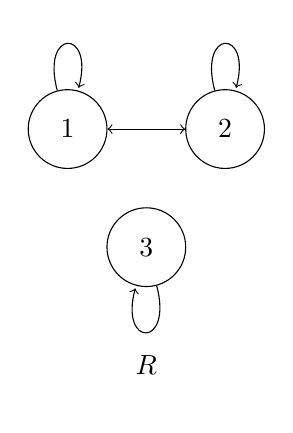
\begin{tikzpicture}[scale=1, every node/.style={circle,draw,minimum size=1cm}]
          \node (1) at (0,1.5) {1};
          \node (2) at (2,1.5) {2};
          \node (3) at (1,0) {3};
          % Reflexive loops
          \draw[->] (1) edge[loop above] ();
          \draw[->] (2) edge[loop above] ();
          \draw[->] (3) edge[loop below] ();
          % Symmetric edges
          \draw[->] (1) -- (2);
          \draw[->] (2) -- (1);
          % Label
          \node[draw=none,fill=none] at (1,-1.5) {$R$};
        \end{tikzpicture}
        \hspace{1cm}
        % S digraph
        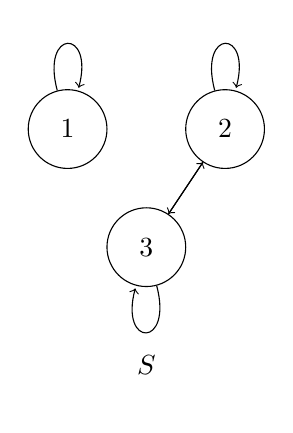
\begin{tikzpicture}[scale=1, every node/.style={circle,draw,minimum size=1cm}]
          \node (1) at (0,1.5) {1};
          \node (2) at (2,1.5) {2};
          \node (3) at (1,0) {3};
          % Reflexive loops
          \draw[->] (1) edge[loop above] ();
          \draw[->] (2) edge[loop above] ();
          \draw[->] (3) edge[loop below] ();
          % Symmetric edges
          \draw[->] (2) -- (3);
          \draw[->] (3) -- (2);
          % Label
          \node[draw=none,fill=none] at (1,-1.5) {$S$};
        \end{tikzpicture}
        \hspace{1cm}
        % R \sOR S digraph
        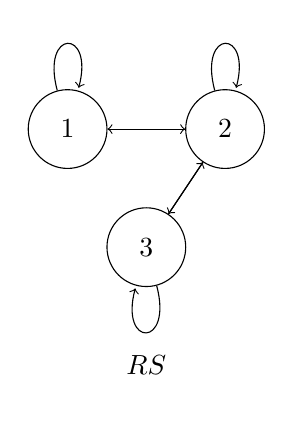
\begin{tikzpicture}[scale=1, every node/.style={circle,draw,minimum size=1cm}]
          \node (1) at (0,1.5) {1};
          \node (2) at (2,1.5) {2};
          \node (3) at (1,0) {3};
          % Reflexive loops
          \draw[->] (1) edge[loop above] ();
          \draw[->] (2) edge[loop above] ();
          \draw[->] (3) edge[loop below] ();
          % Edges from R
          \draw[->] (1) -- (2);
          \draw[->] (2) -- (1);
          % Edges from S
          \draw[->] (2) -- (3);
          \draw[->] (3) -- (2);
          % Label
          \node[draw=none,fill=none] at (1,-1.5) {$R \sOR S$};
        \end{tikzpicture}
        \end{center}
      \end{subdisprove}
    \item The set $R \sAND S$ is an equivalence relation.
      \begin{subprove}
        Let $R$ and $S$ be equivalence relations on a nonempty set $A$. 
        By the definition of \nameref{def:equivalence-relation},
        $R$ and $S$ are reflexive, symmetric, and transitive.
        \begin{itemize}
          \item \textbf{Reflexive:} Since $R$ and $S$ are reflexive by assumption, 
          for all $a \in A$, $(a,a) \in R$ and $(a,a) \in S$. 
          Therefore, $(a,a) \in R \sAND S$ by definition of \nameref{def:set-intersection}.
          \item \textbf{Symmetric:} Let $(a,b) \in R \sAND S$ be arbitrary. 
          Then, $(a,b) \in R$ and $(a,b) \in S$. 
          Since $R$ and $S$ are symmetric by assumption, 
          it follows that $(b,a) \in R$ and $(b,a) \in S$. 
          Therefore, $(b,a) \in R \sAND S$.
          \item \textbf{Transitive:} 
          Let $(a,b), (b,c) \in R \sAND S$ be arbitrary. 
          Then, $(a,b), (b,c) \in R$ and $(a,b), (b,c) \in S$ by definition. 
          Since $R$ and $S$ are transitive by assumption, 
          it follows that $(a,c) \in R$ and $(a,c) \in S$. 
          Therefore, $(a,c) \in R \sAND S$.
        \end{itemize}
        Therefore, $R \sAND S$ is an equivalence relation.
      \end{subprove}
  \end{enumerate}









  \newpage

  \item Let $R$ be a relation on a nonempty set $A$.
  \begin{define}{Symmetry of Relations}[def:symmetry][red]
    Let $A$ be a nonempty set and $R$ a relation on $A$. The relation $R$ is 
    \begin{itemize}
      \item \textbf{Symmetric ($=$)}: For all $x, y \in A$, $(x, y) \in R$ implies $(y, x) \in R$.
        \[
          \forall x, y \in A,\; (x, y) \in R \THEN (y, x) \in R.
        \]
      \item \textbf{Antisymmetric ($\preceq$)}: For all $x, y \in A$, if $(x, y) \in R$ and $(y, x) \in R$, then $x = y$.
        \[
          \forall x, y \in A,\; (x, y) \in R \text{ and } (y, x) \in R \THEN x = y.
        \]
      \item \textbf{Asymmetric ($\prec$)}: For all $x, y \in A$, if $(x, y) \in R$, then $(y, x) \notin R$.
        \[
          \forall x, y \in A,\; (x, y) \in R \THEN (y, x) \notin R.
        \]
    \end{itemize}
    Equivalently, $R$ is asymmetric if and only if $R$ is both antisymmetric and irreflexive.
  \end{define}

  
  \begin{enumerate}
    \item Prove that a relation $R$ on a set $A$ is symmetric if and only if $R=R^{-1}$.
      \begin{subprove}
        Let $R$ be a relation on a nonempty set $A$. 
        The proof is by showing both directions of the biconditional.
        \proofstep
        ($\Rightarrow$) Assume $R$ is symmetric. Let $(a,b) \in R$ be arbitrary. 
        Since $R$ is symmetric by definition of \nameref{def:symmetry}, it follows that $(b,a) \in R$. 
        Therefore, $(a,b) \in R^{-1}$ by definition of \nameref{def:inverse-relation}. 
        Since $(a,b) \in R$ implies $(a,b) \in R^{-1}$, it follows that $R \subseteq R^{-1}$ by definition of subset.
        Conversely, let $(a,b) \in R^{-1}$ be arbitrary. Then, $(b,a) \in R$ by definition of \nameref{def:inverse-relation}. 
        Since $R$ is symmetric, it follows that $(a,b) \in R$. 
        Since $(a,b) \in R^{-1}$ implies $(a,b) \in R$, it follows that $R^{-1} \subseteq R$ by definition of subset.
        Therefore, $R = R^{-1}$.
        \proofstep
        ($\Leftarrow$) Assume $R = R^{-1}$. Let $(a,b) \in R$ be arbitrary. 
        Since $R = R^{-1}$, it follows that $(a,b) \in R^{-1}$. 
        Therefore, $(b,a) \in R$ by definition of \nameref{def:inverse-relation}. 
        Since $(a,b) \in R$ implies $(b,a) \in R$, it follows that $R$ is symmetric by definition.
        \proofstep
        Therefore, $R$ is symmetric if and only if $R = R^{-1}$.
      \end{subprove}
    \item Prove that a relation $R$ on a set $A$ is antisymmetric if and only if $R \sAND R^{-1} \subseteq \Delta$.
    \begin{define}{Diagonal Relation}[def:diagonal-relation][red]
      Let $A$ be a nonempty set. The \textbf{diagonal relation} (or \textbf{identity relation}) on $A$, denoted $\Delta_A$ or $I_A$, is the relation of equality on the set $A$. It is formally defined as the set of all ordered pairs where both components are the same element from $A$:
      $$ \Delta_A = \{ (a,a) \mid a \in A \} $$
    \end{define}
      \begin{subprove}
        Let $R$ be a relation on a nonempty set $A$ and let $\Delta$ be the diagonal relation on $A$ by definition of \nameref{def:diagonal-relation}.
        The proof is by showing both directions of the biconditional.
        \proofstep
        ($\Rightarrow$) Assume $R$ is antisymmetric for the sake of direct proof. 
        Let $(a,b) \in R \sAND R^{-1}$ be arbitrary. 
        Then, $(a,b) \in R$ and $(a,b) \in R^{-1}$ by definition of intersection. 
        Since $(a,b) \in R^{-1}$, it follows that $(b,a) \in R$ by definition of \nameref{def:inverse-relation}. 
        Since $(a,b) \in R$ and $(b,a) \in R$, and $R$ is antisymmetric by definition of \nameref{def:symmetry}, 
        it follows that $a = b$. Therefore, $(a,b) = (a,a) \in \Delta$ by definition of \nameref{def:diagonal-relation}.
        Since $(a,b) \in R \sAND R^{-1}$ implies $(a,b) \in \Delta$, it follows that $R \sAND R^{-1} \subseteq \Delta$ by definition of subset.
        \proofstep
        ($\Leftarrow$) Assume $R \sAND R^{-1} \subseteq \Delta$ for the sake of direct proof. 
        Let $(a,b) \in R$ and $(b,a) \in R$ be arbitrary. 
        Since $(b,a) \in R$, it follows that $(a,b) \in R^{-1}$ by definition of \nameref{def:inverse-relation}. 
        Since $(a,b) \in R$ and $(a,b) \in R^{-1}$, it follows that $(a,b) \in R \sAND R^{-1}$ by definition. 
        Since $R \sAND R^{-1} \subseteq \Delta$, it follows that $(a,b) \in \Delta$ by definition of subset. 
        Therefore, $a = b$ by definition of \nameref{def:diagonal-relation}. 
        Since $(a,b) \in R$ and $(b,a) \in R$ implies $a = b$, it follows that $R$ is antisymmetric by definition.
        \proofstep
        Therefore, $R$ is antisymmetric if and only if $R \sAND R^{-1} \subseteq \Delta$.
      \end{subprove}
  \end{enumerate}


  \newpage
  \item Let $R$ be a relation on the nonempty set $A$. Prove or disprove
  \begin{define}{Reflexivity and Irreflexivity of Relation}[def:reflexivity][red]
    Let $A$ be a nonempty set and $R$ a relation on $A$. The relation $R$ is
    \begin{itemize}
      \item \textbf{reflexive} if and only if
        \[
          \forall x \in A,\; (x, x) \in R.
        \]
      \item \textbf{irreflexive} if and only if
        \[
          \forall x \in A,\; (x, x) \notin R.
        \]
    \end{itemize}
    Equivalently, a relation $R$ is \textbf{irreflexive} if its intersection 
    with the diagonal relation $\Delta_A$ on $A$ is the empty set, 
    i.e., $R \cap \Delta_A = \emptyset$.
  \end{define}
  \begin{enumerate}
    \item The relation $R$ could be neither reflexive nor irreflexive.
      \begin{subprove}
        Let $A = \{1,2\}$ be a nonempty set. Let $R = \{(1,1)\}$ be a relation on $A$. 
        Since $(1,1) \in R$ but $(2,2) \notin R$, it follows that $R$ is not reflexive by definition of \nameref{def:reflexivity}. 
        Since $(1,1) \in R$, it follows that $R$ is not irreflexive by definition of \nameref{def:reflexivity}. 
        Therefore, $R$ is neither reflexive nor irreflexive.
      \end{subprove}



    \item The relation $R$ is reflexive if and only if $\sNOT{R}$ is irreflexive. 
      \begin{subprove}
        Let $R$ be a relation on a nonempty set $A$. 
        The proof is by showing both directions of the biconditional.
        \begin{itemize}
          \item ($\Rightarrow$) Assume $R$ is reflexive. Let $a \in A$ be arbitrary. 
          Since $R$ is reflexive by definition, it follows that $(a,a) \in R$. 
          Therefore, $(a,a) \notin \sNOT{R}$ by definition of complementary set. 
          Since for all $a \in A$, $(a,a) \notin \sNOT{R}$, it follows that $\sNOT{R}$ is irreflexive by definition of \nameref{def:reflexivity}.
          \item ($\Leftarrow$) Assume $\sNOT{R}$ is irreflexive. Let $a \in A$ be arbitrary. 
          Since $\sNOT{R}$ is irreflexive by definition of \nameref{def:reflexivity}, it follows that $(a,a) \notin \sNOT{R}$. 
          Therefore, $(a,a) \in R$. 
          Since for all $a \in A$, $(a,a) \in R$, it follows that $R$ is reflexive by definition.
        \end{itemize}
        Therefore, $R$ is reflexive if and only if $\sNOT{R}$ is irreflexive.
      \end{subprove}
    \item If $R$ is irreflexive, then so is $R^2=R \circ R$.
      \begin{subdisprove}
        Let $A = \{1,2\}$ be a nonempty set. Let $R = \{(1,2),(2,1)\}$ be a relation on $A$. 
        Since $(1,1) \notin R$ and $(2,2) \notin R$, it follows that $R$ is irreflexive by definition of \nameref{def:reflexivity}. 
        However, $R^2 = R \circ R = \{(1,1),(2,2)\}$ by definition of composition. 
        Since $(1,1) \in R^2$ and $(2,2) \in R^2$, it follows that $R^2$ is not irreflexive by definition of \nameref{def:reflexivity}. 
        Therefore, the statement is false by counterexample.
      \end{subdisprove}
  \end{enumerate}


  
  \newpage
  \item Let $[a]_n$ denote the congruence class of $a \in \setZ$ modulo $n$ 
  (that is, the equivalence class of $a$ under the relation congruence modulo $n$) 
  for integers $n \geq 2$. Are the following propositions true or false?
  \begin{enumerate}
    \item $[a]_n = [b]_n \IFF a \equiv b \pmod{n}$
    \begin{subprove}
      
    \end{subprove}
    \item $[a]_n \cap [b]_n \neq \emptyset \IFF a \equiv b \pmod{n}$
    \item $[a]_n \subseteq [b]_n \IFF a \equiv b \pmod{n}$
  \end{enumerate}


  \newpage
  \item Let $R$, $S$, and $T$ be relations on $\setZ$ defined as:~\footnote{
    \textbf{Notice}: The answers contain cross-references throughout this document as clickable hyperlinks in most PDF viewers. 
    However, the Gradescope PDF view might not support clickable hyperlinks.
  }
  \begin{itemize}
    \item $\relation{a}{b}$ if and only if $a \equiv b \pmod{2}$,
    \item $\relation{a}{b}$ (for $S$) if and only if $a \equiv b \pmod{3}$,
    \item $\relation{a}{b}$ (for $T$) if and only if $a \equiv b \pmod{6}$.
  \end{itemize}
  \begin{define}{Congruence Modulo $n$}[def:congruence-modulo-n][red]
    Let $n \in \setZ$ with $n \geq 1$. For $a, b \in \setZ$, $a$ is said to be \textbf{congruent to} $b$ modulo $n$, denoted $a \equiv b \pmod{n}$, if and only if $n$ divides $a-b$:
    \[
      a \equiv b \pmod{n} \iff n \mid (a-b).
    \]
    This relation is defined as an equivalence relation on $\setZ$; its equivalence classes are referred to as \textbf{congruence classes modulo $n$}.
  \end{define} 
  \begin{enumerate}
    \item List the equivalence classes for $R$, $S$, and $T$.
      \begin{subanswer}
        Let $R$, $S$, and $T$ be the relations on $\setZ$ as defined above. The equivalence classes of $R$ are:
        \begin{itemize}
          \item $[0]_R = \{2k \mid k \in \setZ\}$
          \item $[1]_R = \{2k+1 \mid k \in \setZ\}$
        \end{itemize}
        The equivalence classes of $S$ are:
        \begin{itemize}
          \item $[0]_S = \{3k \mid k \in \setZ\}$
          \item $[1]_S = \{3k+1 \mid k \in \setZ\}$
          \item $[2]_S = \{3k+2 \mid k \in \setZ\}$
        \end{itemize}
        The equivalence classes of $T$ are:
        \begin{itemize}
          \item $[0]_T = \{6k \mid k \in \setZ\}$
          \item $[1]_T = \{6k+1 \mid k \in \setZ\}$
          \item $[2]_T = \{6k+2 \mid k \in \setZ\}$
          \item $[3]_T = \{6k+3 \mid k \in \setZ\}$
          \item $[4]_T = \{6k+4 \mid k \in \setZ\}$
          \item $[5]_T = \{6k+5 \mid k \in \setZ\}$
        \end{itemize}
    \end{subanswer}
    \newpage
    \item Find the equivalence classes of $R \sAND S$.
      \begin{subanswer}
        Let $R$ and $S$ be the relations on $\setZ$ as defined above. 
        Since $R \sAND S$ is the relation where $a (R \sAND S) b$ if and only if $a \equiv b \pmod{2}$ and $a \equiv b \pmod{3}$, 
        it follows that $R \sAND S$ is congruence modulo $6$ by the Chinese Remainder Theorem. 
        Therefore, the equivalence classes of $R \sAND S$ are:
        \begin{itemize}
          \item $[0]_{R \sAND S} = \{6k \mid k \in \setZ\}$
          \item $[1]_{R \sAND S} = \{6k+1 \mid k \in \setZ\}$
          \item $[2]_{R \sAND S} = \{6k+2 \mid k \in \setZ\}$
          \item $[3]_{R \sAND S} = \{6k+3 \mid k \in \setZ\}$
          \item $[4]_{R \sAND S} = \{6k+4 \mid k \in \setZ\}$
          \item $[5]_{R \sAND S} = \{6k+5 \mid k \in \setZ\}$
        \end{itemize}
      \end{subanswer}


    \item Prove the partition resulting from $T$ is a refinement of the partition resulting from $S$.
\begin{define}{Partition Refinement}[def:partition-refinement][red]
  Let $A$ be a nonempty set, and let $\mathcal{P}_1$ and $\mathcal{P}_2$ be 
  two partitions of $A$. The partition $\mathcal{P}_1$ is said to be a 
  \emph{refinement} of $\mathcal{P}_2$ if and only if every block of 
  $\mathcal{P}_1$ is a subset of some block of $\mathcal{P}_2$. 
  This relationship can be expressed symbolically as:
  $$ \forall S_1 \in \mathcal{P}_1, \; \exists S_2 \in \mathcal{P}_2 \text{ such that } S_1 \subseteq S_2 $$
\end{define}
      \begin{subprove}
        Let $T$ and $S$ be the relations on $\setZ$ as defined above. 
        To show that the partition resulting from $T$ is a refinement of the partition resulting from $S$, 
        it is required to show that every equivalence class of $T$ is contained in some equivalence class of $S$ by definition of \nameref{def:partition-refinement}.
        Let $[k]_T$ be an arbitrary equivalence class of $T$ where $0 \leq k < 6$. 
        Since $a \in [k]_T$ if and only if $a \equiv k \pmod{6}$ by definition of \nameref{def:equivalence-relation}, 
        and since $a \equiv k \pmod{6}$ implies $a \equiv k \pmod{3}$, 
        it follows that $a \in [k \bmod 3]_S$. 
        Therefore, $[k]_T \subseteq [k \bmod 3]_S$ by definition of subset. 
        Since this holds for all equivalence classes of $T$, it follows that the partition resulting from $T$ is a refinement of the partition resulting from $S$ by definition of \nameref{def:partition-refinement}.
      \end{subprove}
    \item What is the relationship between the partition resulting from $T$ and the partition resulting from $R$? Justify your answer.
      \begin{subanswer}
        Let $T$ and $R$ be the relations on $\setZ$ as defined above. 
        The partition resulting from $T$ is a refinement of the partition resulting from $R$. 
        This is because for each equivalence class $[k]_T$ of $T$ where $0 \leq k < 6$, 
        since $a \in [k]_T$ if and only if $a \equiv k \pmod{6}$ by definition of \nameref{def:equivalence-relation}, 
        and since $a \equiv k \pmod{6}$ implies $a \equiv k \pmod{2}$, 
        it follows that $a \in [k \bmod 2]_R$. 
        Therefore, $[k]_T \subseteq [k \bmod 2]_R$ by definition of subset, 
        and the partition resulting from $T$ is a refinement of the partition resulting from $R$ by definition of \nameref{def:partition-refinement}.
      \end{subanswer}
    \item What is the relationship between $S$ and $T$? Between $R$ and $T$? Justify your answers.
      \begin{subanswer}
        Let $R$, $S$, and $T$ be the relations on $\setZ$ as defined above. 
        Since congruence modulo $6$ implies congruence modulo $3$ and congruence modulo $2$, 
        it follows that $T \subseteq S$ and $T \subseteq R$ by definition of subset. 
        However, $S \not\subseteq T$ and $R \not\subseteq T$ since congruence modulo $3$ does not imply congruence modulo $6$, 
        and congruence modulo $2$ does not imply congruence modulo $6$.
      \end{subanswer}
    \item Is there any relationship between $R$ and $S$? Justify your answers.
      \begin{subanswer}
        Let $R$ and $S$ be the relations on $\setZ$ as defined above. 
        Since congruence modulo $2$ does not imply congruence modulo $3$ and congruence modulo $3$ does not imply congruence modulo $2$, 
        it follows that $R \not\subseteq S$ and $S \not\subseteq R$ by definition of subset. 
        Since $R \neq S$ (they have different equivalence classes), 
        it follows that $R$ and $S$ are independent equivalence relations with no subset relationship between them.
      \end{subanswer}
  \end{enumerate}
\end{enumerate}


























\newpage\handout[true]
{\textsc{Math 2106-B: Foundations of Mathematical Proof}}{Fall 2025}
{Homework 5: Functions}
{\textit{Prof.} \href{https://ceheitsch.github.io/webpage/}{Dr. Christine Heitsch}}{Due Date: October 2nd}
{Math 2106-B: HW5}
{\large
  \noindent
  \textbf{Name:} \HandoutAuthor \smallskip \\

  \noindent
  \textbf{GTID:} 903743506 \smallskip \\

  \noindent
  %%% List anyone with whom you discussed the problems
  \textbf{Collaborators:} None. This material reflects independent preparation. \smallskip \\

  \noindent
  %%% List all resources used OTHER than the textbook, lecture notes, 
  %%% webwork problems, ICA questions, and previous homework assignments.
  \textbf{Outside resources:} This work was informed by MATH 2106 course materials 
  (ICAs: in-class activities and WebWork contents) from \HandoutInstitution\ (the course textbook is 
  Chartrand \parencite{chartrand_mathematical_2018}).   
  Outside references specifically include
  textbooks written by 
  Grimaldi \parencite{grimaldi_discrete_2004} (used in MATH 3012) and 
  Rosen \parencite{rosen_discrete_2019} (used in CS 2050). \smallskip \\

  \noindent
  \textbf{Notice}: The answers contain cross-references throughout this document as clickable hyperlinks in most PDF viewers. However, the Gradescope PDF view might not support clickable hyperlinks.
}\newpage
% \printbibliography[
  heading=bibintoc,   
  title={References}     % change “References” text if needed
]
% `heading=bibnumbered` if you prefer it numbered chapter (in \tableofcontents)
% `heading=bibintoc`    if you prefer it unnumbered but still in the ToC\newpage
% The following table presents the standard logical equivalences from these sources together with 
the author's own (or the student, myself, Jaehoon Song) clarifications and labels where applicable.


\begin{table}[h!]
  \centering
  \renewcommand{\arraystretch}{1.2}
  \setlength{\tabcolsep}{8pt}
  \begin{tabular}{|p{5.0cm}|p{5.0cm}|p{5.2cm}|}
    \hline
    \rowcolor[HTML]{E0E0E0}
    \multicolumn{2}{|l|}{\textbf{Logical Equivalences}} & \textbf{Name} \\
    \hline
    $\,p \AND q \equiv q \AND p$ & $\,p \OR q \equiv q \OR p$ & Commutative Law \\
    \hline
    $\, (p \AND q) \AND r \equiv p \AND (q \AND r)$ & $\, (p \OR q) \OR r \equiv p \OR (q \OR r)$ & Associative Law \\
    \hline
    $\,p \AND (q \OR r) \equiv (p \AND q) \OR (p \AND r)$ & $\,p \OR (q \AND r) \equiv (p \OR q) \AND (p \OR r)$ & Distributive Law \\
    \hline
    $\,\overline{p \AND q} \equiv \sNOT{p} \OR \sNOT{q}$ & $\,\overline{p \OR q} \equiv \sNOT{p} \AND \sNOT{q}$ & DeMorgan's Law \\
    \hline
    \multicolumn{2}{|l|}{$\,\overline{\overline{p}} \equiv p$} & Double Negation law \\
    \hline
    $\,p \AND \boldsymbol{T} \equiv p$ & $\,p \OR \boldsymbol{F} \equiv p$ & Identity Law \\
    \hline
    $\,p \OR \boldsymbol{T} \equiv \boldsymbol{T}$ & $\,p \AND \boldsymbol{F} \equiv \boldsymbol{F}$ & Domination Law \\
    \hline
    $\,p \AND p \equiv p$ & $\,p \OR p \equiv p$ & Idempotent Law \\
    \hline
    \multicolumn{2}{|l|}{$\,p \THEN q \equiv \sNOT{p} \OR q$} & Implication Equivalence \\
    \hline
    \multicolumn{2}{|l|}{$\,\overline{p \THEN q} \equiv p \AND \sNOT{q}$} & Negation of Implication \\
    \hline
    \multicolumn{2}{|l|}{$\,p \THEN q \equiv \sNOT{q} \THEN \sNOT{p}$} & Contrapositive Equivalence \\
    \hline
    \multicolumn{2}{|l|}{$\,p \OR \sNOT{p} \equiv \boldsymbol{T}$} & Law of Tautology \\
    \hline
    \multicolumn{2}{|l|}{$\,p \AND \sNOT{p} \equiv \boldsymbol{F}$} & Law of Contradiction \\
    \hline
  \end{tabular}
\end{table}\newpage
% 
The following definitions are presented from standard mathematical sources (\textbf{Sets}).
Clarifications and labels have been added where applicable.

\begin{define}{Basic Set Concepts}\phantomsection\label{def:basic-set-concepts} % \hyperref[def:basic-set-concepts]{YOUR_CONTEXT}
  \begin{enumerate}
    \item \textbf{Universal Set:} A universal set $\setUNIV$ is a
    set that contains all objects under consideration in a particular context or problem.
    \item \textbf{Empty Set:} The empty set, denoted $\setNULL$,
    is the unique set that contains no elements.
    \item \textbf{Subset:} Let $A$ and $B$ be sets. $A$ is a
    subset of $B$ ($A \subseteq B$) if (and only if)
    for all $x \in A$, $x \in B$.
    \item \textbf{Set Equality:} Let $A$ and $B$ be sets. The sets $A$ and $B$ are
    equal ($A = B$) if $A \subseteq B$ and $B \subseteq A$.
    \item \textbf{Power Set:} Let $A$ be a set. The power set of $A$, denoted $\sPOWER{A}$ or $2^A$,
    is the set of all subsets of $A$. That is, $\mathcal{P}(A) = \{S\in\setUNIV : S \subseteq A\}$.
  \end{enumerate}
\end{define}
The following definitions extend the understanding of set operations
and properties.


\begin{define}{Set Operations}\phantomsection\label{def:set-operations} % \hyperref[def:set-operations]{YOUR_CONTEXT}
  \begin{enumerate}
    \item \textbf{Complementary Set:} Let $A$ be a subset of the universal set $\setUNIV$.
    The complement of $A$, denoted $A^c$ or $\overline{A}$, is the set of all elements
    in $\setUNIV$ that are not in $A$. That is, $A^c = \{x \in \setUNIV : x \notin A\}$.
    \item \textbf{Union:} Let $A$ and $B$ be sets. The union of $A$ and $B$,
    denoted $A \cup B$, is the set of all elements that are in $A$, or in $B$, or in both.
    That is, $A \cup B = \{x : x \in A \lor x \in B\}$.
    \item \textbf{Intersection:} Let $A$ and $B$ be sets. The intersection of $A$ and $B$,
    denoted $A \cap B$, is the set of all elements that are in both $A$ and $B$.
    That is, $A \cap B = \{x : x \in A \land x \in B\}$.
    \item \textbf{Set Difference:} Let $A$, $B$ be subsets of a universal set $\setUNIV$.
    The set difference $A \sMINUS B$ is defined to be the set
    $\{ x \in \setUNIV \LDIV x \in A \text{ and } x \notin B\}$. \vspace*{10px}\\
    \textit{It is sometimes called the relative complement of $B$ in $A$,
    and denoted in the textbook as $A - B$.}
    \item \textbf{Cartesian Product:} Let $A$ and $B$ be sets. The Cartesian product of
    $A$ and $B$, denoted $A \sTIMES B$, is the set consisting of all ordered pairs:
    \[
    A \sTIMES B = \{(a, b) \LDIV a \in A, b \in B\}.
    \]
  \end{enumerate}
\end{define}


\newpage

The following claims are given in the reference as well. Let $A,B\in U$, a universal set.


\begin{claim}{Subset of Union: $A \subseteq \sOR{A}{B}$}\phantomsection\label{claim:subset-union} % \hyperref[claim:subset-union]{YOUR_CONTEXT}
  \begin{subprove}[bluecolor]
      Let $x\in U$, assume $x\in A$. Then the statement \inlinequote{$x\in A$ or $x\in B$} is true.
      Hence, by the definition, $\sOR{A}{B}=\{x\in U\LDIV x\in A$ or $x\in B\}$, $x\in \sOR{A}{B}$.
      Thus, $A \subseteq \sOR{A}{B}$.
  \end{subprove}
\end{claim}

\begin{claim}{Empty Subset: $\setNULL \subseteq A$}\phantomsection\label{claim:empty-subset} % \hyperref[claim:empty-subset]{YOUR_CONTEXT}
  \begin{subprove}[bluecolor]
      Let $x\in U$, assume $x\in \setNULL$. But there are no elements in $\setNULL$, so
      $x\in \setNULL$ is false. Since the premise is false, the implication if $x\in \setNULL$,
      then $x\in A$ is true. Thus, $\setNULL \subseteq A$ by definition of \hyperref[def:basic-set-concepts]{subsets}.
  \end{subprove}
\end{claim}

\begin{claim}{Subset as Equality: $\sOR{A}{B}=A$ if and only if $B\subseteq A$}\phantomsection\label{claim:subset-equality} % \hyperref[claim:subset-equality]{YOUR_CONTEXT}
  \begin{subprove}[bluecolor]
      Let $x\in U$, first, we assume $B\subseteq A$, we have already shown
      $A \subseteq \sOR{A}{B}$ by the claim, \hyperref[claim:subset-union]{Subset of Union}. 
      To show $\sOR{A}{B} \subseteq A$, assume $x\in \sOR{A}{B}$.
      By definition, $x\in A$ or $x\in B$. Considering $x\in B$ and assumption
      $B \subseteq A$, $x\in B$ implies $x\in A$. Thus, $\sOR{A}{B} \subseteq A$.
      Hence, if $B\subseteq A$, then $\sOR{A}{B} = A$. \vspace*{10px}\\
      Now, we assume $\sOR{A}{B}=A$. To show $B\subseteq A$, we now assume $x\in B$. Since $x\in B$, by definition
      of union, $x\in \sOR{A}{B} = A$. Therefore, $B\subseteq A$.
  \end{subprove}
\end{claim}


%%%%%%%%%%%%%%%%%%% 9/8/25

Let $\setUNIV$ be a set. 
\begin{claim}{ICA6}\phantomsection\label{claim:ica6} % \hyperref[claim:ica6]{YOUR_CONTEXT}
  For all $A,B\in\setUNIV$, $$A\sTIMES B =\setNULL\THEN \group{A=\setNULL\OR B=\setNULL}$$
  \begin{subprove}[bluecolor]
    Let $A,B\in\setUNIV$. We prove $A\sTIMES B=\setNULL$. Assume it is not the case that 
    $A=\setNULL$ or $B=\setNULL$. Thus, we have $A=\setNULL$ and $B=\setNULL$. 
    Since $A\ne\setNULL$ by assumption, there exists an element $a\in A$. Likewise, there 
    is some $b\in B$ since $B\ne\setNULL$. Thus, $\group{a,b}\in\sBUILD{(x,y)}{x\in A,y\in B}$ 
    by definition. But then, $A\sTIMES B\ne\setNULL$ by definition. Hence, the claim holds. 
  \end{subprove}
\end{claim}


\begin{define}{Relatively Prime Integers (Coprime)}\phantomsection\label{def:relatively-prime} % \hyperref[def:relatively-prime]{YOUR_CONTEXT}
  Let $x,y \in \mathbb{Z}$. The integers $x$ and $y$ are said to be
  \textbf{relatively prime} if and only if
  $\gcd(x,y) = 1$.
\end{define}
\newpage
% The following definitions and axioms are presented from standard mathematical sources (\textbf{Number Theory}) together with the author's own (or the student, myself, Jaehoon Song) clarifications and labels where applicable.

\begin{define}{Integers}[def:integers][red]
  $\setZ$: the set of all integers
\end{define}

\begin{define}{Rational Numbers}[def:rational-numbers][red]
  $\setQ$: the set of all rational numbers
\end{define}

\begin{define}{Real Numbers}[def:real-numbers][red]
  $\setR$: the set of all real numbers
\end{define}

\begin{define}{Natural Numbers}[def:natural-numbers][red]
  $\setN$ or $\setZ_{>0}$: the set of all natural numbers which are the set of positive integers (not including $0$)
\end{define}

\begin{define}{Positive Real Numbers}[def:positive-real-numbers][red]
  $\setR_{>0}$: the set of all positive real numbers
\end{define}

\begin{define}{Non-negative Real Numbers}[def:non-negative-real-numbers][red]
  $\setR_{\geq 0}$: the set of all non-negative real numbers
\end{define}


\newpage

The following definitions and claims extend the understanding of integers.

Here are the ICA2 Definitions and Axioms as follows.

\begin{define}{Even Integer}[def:even-integer][red]
  An integer $n$ is \underbar{even} if there exists 
  (existential quantification logic $\exists$) an integer $k$ such that
  \[
  n = 2k.
  \]
\end{define}

\begin{define}{Odd Integer}[def:odd-integer][red]
  An integer $n$ is \underbar{odd} if 
  there exists some integer $k$ such that
  \[
  n = 2k + 1.
  \]
\end{define}

\begin{define}{Closure under Addition}[def:closure-addition][red]
  The sum of two integers is again an 
  integer. (Closure under addition)
\end{define}

\begin{define}{Closure under Multiplication}[def:closure-multiplication][red]
  The product of two integers is again 
  an integer. (Closure under multiplication)
\end{define}

\begin{define}{Odd if and only if Not Even}[def:odd-iff-not-even][red]
  An integer is odd if and only if it 
  is not even.
\end{define}

Here are the ICA3 Definitions and Axioms as follows.

\begin{define}{Universal Closure under Addition}[def:universal-closure-addition][red]
  The sum of two integers (Universal quantification for all, for every, for each) is again an integer. (Closure under addition)
\end{define}

\begin{define}{Universal Closure under Multiplication}[def:universal-closure-multiplication][red]
  The product of two integers (Universal quantification for all, for every, for each) is again an integer. (Closure under multiplication)
\end{define}

\begin{define}{Even Integer Square}[def:even-integer-square][red]
  An integer $n$ is even if and only if $n^2$ is even.
\end{define}

\newpage

The following claims are given in the reference as well.

\begin{define}{Sum of Even Integers}[claim:sum-even-integers][red]
  The sum of two even integers is again an even integer.
  \begin{subprove}[red]
    Let $x$ be an integer and $y$ be an integer ($\forall x,y \in \setZ$). 
    Suppose $x$ is even and $y$ is even. Then, by \nameref{def:even-integer}, there exists an integer 
    $k$ and an integer $j$ such that $x=2k$ and $y=2j$. Then, 
    $x+y=\left(2k\right)+\left(2j\right)=2\left(k+j\right)$. By \nameref{def:closure-addition}, since $k$ and 
    $j$ are integers, then so is $\left(k+j\right)$. Hence, by definition, $x+y$ is an 
    even integer.
  \end{subprove}
\end{define}

The following definitions extend the understanding of integers including divisibility.

\begin{define}{Divisibility}[def:divisibility][red]
  An integer $n$ divides an integer $m$, denoted $n \LDIV m$, if there 
  exists an integer $k$ such that $m=n k$. Otherwise, $n \nmid m$.
\end{define}

The following definitions extend the classification of real numbers into rational and irrational numbers.

\begin{define}{Rational Number}[def:rational-number][red]
  A real number $x$ is \underbar{rational} if there exist integers $a$ and $b$ with $b \neq 0$ such that $bx = a$.
  Otherwise, $x$ is \underbar{irrational}.

  \textbf{Note}: Compare the rational number definition with the even/odd axiom \inlinequote{odd iff not even} from \nameref{def:odd-iff-not-even}.
\end{define}

The following claims are given in the reference as well.

\begin{define}{Irrationality of $\sqrt{2}$}[claim:sqrt2-irrational][red]
  $\sqrt{2}$ is irrational.
  \begin{subprove}[red]
    Suppose $\sqrt{2}$ is rational. Then, by \nameref{def:rational-number}, there exists $a,b\in \setZ$ 
    with $b\ne 0$ such that $b\cdot\sqrt{2}=a$. We may further assume that any factors 
    common to $a$ and $b$ have already been removed.\\

    Then, squaring both sides, this yields $2\cdot b^2 = a^2$.
    Since products of integers are again integers by \nameref{def:closure-multiplication}, we have that $a^2,b^2\in \setZ$.
    Thus, by definition, $a^2$ is even. Therefore, by \nameref{def:even-integer-square}, $a$ is even. 
    Thus, there exists $c\in\setZ$ such that $a=2c$. Then
    $$
    2b^2=a^2={2c}^2=4c^2
    $$
    Then, $b^2=2c^2$. Then, as before, $b^2$ is even, so $b$ is even.
    However, $a$ and $b$ both being even contradicts the fact that any factors 
    common to $a$ and $b$ have already been removed.
  \end{subprove}
\end{define}






%%%%%%%%%%%%%%%%%%% New style (refactor model)
\begin{define}{Relatively Prime Integers (Coprime)}[def:relatively-prime][red]
  Let $x,y \in \mathbb{Z}$. The integers $x$ and $y$ are said to be
  \textbf{relatively prime} if and only if
  $\gcd(x,y) = 1$.
\end{define}\newpage






%%%%%%%%%%%%%%%%%%%%%%%%%%%%%%%%%%%%%%%%%%%%%%%%%%%%%%%%%%%%%%%%%%%%%%%
% References
%%%%%%%%%%%%%%%%%%%%%%%%%%%%%%%%%%%%%%%%%%%%%%%%%%%%%%%%%%%%%%%%%%%%%%%
\textbf{Remark}: The following definitions (or results) are already proved in class or on previous ICA, 
Wbwk, Hmwk assignments, and contents of the textbook.

\begin{define}{One-to-One Correspondence (Bijective Function)}[def:bijective][red]
  Let $f : A \to B$ be a function. $f$ is \textbf{bijective} if and only if it is both injective and surjective.
\end{define}

\begin{define}{Theorem (Existence of Inverse)}[thm:inverse-function][red]
  The inverse relation $f^{-1}$ is a function if and only if $f$ is both injective and surjective.
  \begin{subprove}
    We consider the inverse relation $f^{-1} \subseteq B \times A$ for the function 
    \[
    f : A \to B \quad \text{on nonempty sets $A,B$.}
    \]
    Assume $f$ is a bijection, i.e., both one-to-one and onto. Let $b \in B$. Since $f$ is onto, by definition, there exists $a \in A$ with $f(a) = b$. So $(a,b) \in f$ and $(b,a) \in f^{-1}$. Hence for all $b \in B$ there exists $a \in A$ such that $(b,a) \in f^{-1}$. 

    Now let $a, a' \in A$. Suppose $(b,a) \in f^{-1}$ and $(b,a') \in f^{-1}$. 
    Then $(a,b), (a',b) \in f$, so $f(a) = b$ and $f(a') = b$. 
    But $f$ is one-to-one by assumption, and so $a = a'$. 
    Hence we have shown that each $b \in B$ has at least one image under 
    the inverse relation $f^{-1}$ and no more than one. 
    Thus the inverse relation is a function whenever $f$ is a bijection.

    \medskip
    Conversely, \dots
  \end{subprove}
  % \begin{subprove}
  %   ($\Rightarrow$) Assume $f^{-1}$ is a function. To show $f$ is injective, let $a_1, a_2 \in A$ such that $f(a_1) = f(a_2)$. 
  %   Then, $(a_1, f(a_1)) \in f$ and $(a_2, f(a_2)) \in f$. Since $f^{-1}$ is a function, $(f(a_1), a_1) \in f^{-1}$ and $(f(a_2), a_2) \in f^{-1}$. 
  %   By the definition of a function, $a_1 = a_2$. Thus, $f$ is injective.
    
  %   To show $f$ is surjective, let $b \in B$. Since $f^{-1}$ is a function, there exists an $a \in A$ such that $(b, a) \in f^{-1}$. 
  %   By the definition of inverse relation, $(a, b) \in f$, so $f(a) = b$. Thus, $f$ is surjective.
    
  %   ($\Leftarrow$) Assume $f$ is both injective and surjective. To show $f^{-1}$ is a function, let $(b, a_1), (b, a_2) \in f^{-1}$. 
  %   Then, $(a_1, b), (a_2, b) \in f$. Since $f$ is injective, it follows that $a_1 = a_2$. Thus, $f^{-1}$ satisfies the definition of a function.
  % \end{subprove}

\end{define}






\newpage













%%%%%%%%%%%%%%%%%%%%%%%%%%%%%%%%%%%%%%%%%%%%%%%%%%%%%%%%%%%%%%%%%%%%%%%
% Problems
%%%%%%%%%%%%%%%%%%%%%%%%%%%%%%%%%%%%%%%%%%%%%%%%%%%%%%%%%%%%%%%%%%%%%%%
\begin{enumerate} 
  \item Let $X, Y$, and $Z$ be nonempty sets with $A, B \subseteq X$ and $C, D \subseteq Y$. 
  Let $f: X \rightarrow Y$ and $g: Y \rightarrow Z$ be functions. 
  Prove the following statements or give the required counterexample.
  \begin{enumerate}
    \item Prove that if $f$ and $g$ are one-to-one, then so is $g \circ f$.
    \begin{define}{One-to-One (Injective Function)}[def:injective][red]
      Let $f : A \to B$ be a function. $f$ is \textbf{injective} (one-to-one) if and only if for all $a_1, a_2 \in A$, if $f(a_1) = f(a_2)$, then $a_1 = a_2$.
    \end{define}
    \begin{subprove}
      Suppose $f$ and $g$ are \nameref{def:injective} for the sake of direct proof.\proofstep
      Let $x_1, x_2 \in A$ be arbitrary such that $(g \circ f)(x_1) = (g \circ f)(x_2)$.
      By the definition of function composition, it follows that $$g(f(x_1)) = g(f(x_2)).$$
      By assumption, the function $g$ is one-to-one, it follows that $f(x_1) = f(x_2)$.
      Furthermore, $f$ is also one-to-one, it follows that $x_1 = x_2$.\proofstep
      Therefore, the function $g \circ f$ is one-to-one by definition.
    \end{subprove}
    \item Prove that if $g \circ f$ is one-to-one, then so is $f$.
    \begin{subprove}
      Assume $g \circ f$ is \nameref{def:injective}. Suppose $f$ is not one-to-one 
      for the sake of contradiction. \proofstep
      Let $x_1, x_2 \in A$ be arbitrary. Since $f$ is not one-to-one, 
      there exist $x_1, x_2 \in A$ such that $x_1 \neq x_2$ and $f(x_1) = f(x_2)$. 
      By the definition of function composition and the assumption, $$(g \circ f)(x_1) = g(f(x_1)) = g(f(x_2)) = (g \circ f)(x_2).$$
      Then, $x_1 = x_2$ since $g \circ f$ is one-to-one, which contradicts the assumption, $x_1 \neq x_2$. Therefore, $f$ must be one-to-one.
    \end{subprove}
    \newpage
    \item Prove that if $f$ is onto and $g \circ f$ is one-to-one, then $g$ is one-to-one.
    \begin{define}{Onto (Surjective Function)}[def:surjective][red]
      Let $f : A \to B$ be a function. $f$ is \textbf{surjective} (onto) if and only if for every $b \in B$, there exists $a \in A$ such that $f(a) = b$.
    \end{define}
    \begin{subprove}
      Let $y_1, y_2 \in Y$ be arbitrary elements. 
      Assume $f$ is \nameref{def:surjective} and $g \circ f$ is \nameref{def:injective} 
      for the sake of direct proof.\proofstep
      Suppose $y_1, y_2 \in Y$ be arbitrary such that $g(y_1) = g(y_2)$.
      Then, there exist $x_1, x_2 \in X$ such that 
      $f(x_1) = y_1$ and $f(x_2) = y_2$ for $y_1, y_2 \in Y$ since $f$ is onto by assumption. 
      Thus, by substitution, $g(f(x_1)) = g(f(x_2))$.
      Moreover, it implies $x_1 = x_2$ since $g \circ f$ is one-to-one. 
      \begin{define}{Function}[def:function][red]
        Let $A$ and $B$ be nonempty sets. A \textbf{function} $f$ from $A$ to $B$, denoted $f : A \to B$, 
        is a relation, $f\in A\sTIMES B$ such that 
        \begin{enumerate}
          \item For every $a \in A$, there exists an element $b \in B$ such that $f(a) = b$.
          \item For every $a \in A$ and for all $b, c \in B$, if $f(a) = b$ and $f(a) = c$, then $b = c$.
        \end{enumerate}
        where the set $A$ is called the \textbf{domain} of $f$, 
        and the set $B$ is called the \textbf{codomain} of $f$.
        If $f(a)=b$, then $b$ is called the \textbf{image} of $a$ under $f$.
        The function maps $a$ to $b$, and $f$ is often called a \textbf{mapping}.
      \end{define}
      \begin{define}{Domain and Codomain}[def:domain-codomain][red]
        If $f : A \to B$ is a function, then $A$ is called the \textbf{domain} of $f$, and $B$ is called the \textbf{codomain} of $f$.
      \end{define}
      By the definition of \nameref{def:function}, there must be a mapping of $x$ to $y$ in \nameref{def:domain-codomain} such that
      $$y_1 = f(x_1) = f(x_2) = y_2.$$
      Thus, $g$ is one-to-one by definition.\proofstep
      Therefore, by direct proof, $f$ is onto and $g \circ f$ is one-to-one only if $g$ is one-to-one.
    \end{subprove}
    \newpage
    \item Give an example where $g \circ f$ is one-to-one, but $g$ is not.
    \begin{subanswer}
      Let $X=\{1,2\}, Y=\{3,4,5\}, Z=\{6,7\}$. 
      Let $f: X \rightarrow Y$ and $g: Y \rightarrow Z$ be functions defined as follows for the sake of counterexample.
      \[
        f(1)=3, \quad f(2)=4; \qquad g(3)=6, \quad g(4)=7, \quad g(5)=7.
      \]
      % Diagram of f and g and g o f
      diagramed as follows. \label{prob:1d}
      \[
        \xymatrix@R=2em@C=2em{
          X \xyArc[r]^{f}   & Y \xyArc[r]^{g}   & Z \\
          \{1\} \xyArc[r]   & \{3\} \xyArc[r]   & \{6\} \\
          \{2\} \xyArc[r]   & \{4\} \xyArc[r]   & \{7\} \\
          {}                & \{5\} \xyArc[ur]  & {} \\
        }
      \]
      Then, the composition $g \circ f$ is one-to-one since 
      $(g \circ f)(1) = g(f(1)) = g(3) = 6$ and $(g \circ f)(2) = g(f(2)) = g(4) = 7$ which follows the definition of \nameref{def:injective}.
      However, $g$ is not one-to-one since $g(4) = 7$ and $g(5) = 7$, but $4 \neq 5$.\proofstep
      Therefore, by counterexample, there exists a case that $g \circ f$ is one-to-one, but $g$ is not.
    \end{subanswer}
  \end{enumerate}



  \newpage
  \item Let $X, Y$, and $Z$ be nonempty sets with $A, B \subseteq X$ and $C, D \subseteq Y$. 
  Let $f: X \rightarrow Y$ and $g: Y \rightarrow Z$ be functions. 
  Prove the following statements or give the required counterexample.
  \begin{enumerate}
    \item Prove that if $f$ and $g$ are onto, then so is $g \circ f$.
    \begin{subprove}
      Let $z \in Z$ be an arbitrary image for $g \circ f$. 
      Then, assume $f$ and $g$ are onto for the sake of direct proof.
      By definition of \nameref{def:surjective}, 
      there exists $x \in X$ such that $f(x) = y$ since $f$ is onto.
      Also, there exists $y \in Y$ such that $g(y) = z$ since $g$ is onto.\proofstep
      Thus, for any $z \in Z$, there exists $x \in X$ such that $(g \circ f)(x) = z$.
      Therefore, $g \circ f$ is onto by definition.
    \end{subprove}
    \item Prove that if $g \circ f$ is onto, then so is $g$.
    \begin{subprove}
      Let $z \in Z$ be an arbitrary image for $g \circ f$. 
      Assume $g \circ f$ is onto for the sake of direct proof.
      By definition of \nameref{def:surjective}, 
      there exists $x \in X$ such that $(g \circ f)(x) = z$.
      Moreover, there exists $y \in Y$ such that $f(x) = y$ since $f$ is a \nameref{def:function}.
      By substitution, $g(y) = z$.\proofstep
      Thus, for any $z \in Z$, there exists $y \in Y$ such that $g(y) = z$.
      Therefore, $g$ is onto by definition.
    \end{subprove}
    \item Prove that if $g$ is one-to-one and $g \circ f$ is onto, then $f$ is onto.
    \begin{subprove}
      Let $y \in Y$ be an arbitrary image for $f$. 
      Assume $g$ is \nameref{def:injective} and $g \circ f$ is \nameref{def:surjective} for the sake of direct proof.
      By definition, there exists $z \in Z$ such that $g(y) = z$ since $g$ is a \nameref{def:function}.
      Moreover, there exists $x \in X$ such that $(g \circ f)(x) = z$ for the $z$ since $g \circ f$ is onto.
      It follows that 
      $$g(f(x)) = g(y) = z$$
      which implies $f(x) = y$ since $g$ is \nameref{def:injective}.\proofstep
      Thus, for any $y \in Y$, there exists $x \in X$ such that $f(x) = y$.
      Therefore, $f$ is onto by definition.
    \end{subprove}
    \item Give an example where $g \circ f$ is onto, but $f$ is not.
    \begin{subanswer}
      Let $X=\{1,2\}, Y=\{3,4,5\}, Z=\{6,7\}$. 
      Let $f: X \rightarrow Y$ and $g: Y \rightarrow Z$ be functions defined as follows for the sake of counterexample.
      \[
        f(1)=3, \quad f(2)=4; \qquad g(3)=6, \quad g(4)=7, \quad g(5)=7.
      \]
      It has been already diagramed in the previous problem, \parenref{prob:1d}.
      Then, the composition $g \circ f$ is onto since 
      $(g \circ f)(1) = g(f(1)) = g(3) = 6$ and $(g \circ f)(2) = g(f(2)) = g(4) = 7$ which follows the definition of \nameref{def:surjective}.
      However, $f$ is not onto since there is no $x \in X$ such that $f(x) = 5$.\proofstep
      Therefore, by counterexample, there exists a case that $g \circ f$ is onto, but $f$ is not.
    \end{subanswer}
  \end{enumerate}


  \newpage 
  \item Let $X, Y$, and $Z$ be nonempty sets with $A, B \subseteq X$ and $C, D \subseteq Y$. 
  Let $f: X \rightarrow Y$ and $g: Y \rightarrow Z$ be functions. 
  Prove the following statements.
  \textbf{Remark}: Let $A$ and $B$ be arbitrary sets. By definition of \nameref{def:set-equality}, 
  $A = B$ requires showing both directions of \nameref{def:subset}s, $A \subseteq B$ and $B \subseteq A$.
  \begin{define}{Image and Inverse Image}[def:image][red]
    Let $f : X \to Y$ be a function, $C\subseteq X$, and $D\subseteq Y$. 
    \begin{enumerate}
      \item The \textbf{image} $f(C)$ is the set $\{y=f(c) \in Y : c \in C\} \subseteq Y$.
      \item The \textbf{inverse image} $f^{-1}(D)$ is the set $\{x \in X : y=f(x) \in D\} \subseteq X$.
    \end{enumerate}
  \end{define} 
  \begin{enumerate}
    \item $f(A \sOR B)=f(A) \sOR f(B)$ \label{prob:3a}
    \begin{subprove}
      ($\subseteq$) Let $y \in f(A \sOR B)$ be arbitrary. Then, by definition of \nameref{def:image}, 
      there exists $x \in A \sOR B$ such that $f(x) = y$.      
      \begin{define}{Set Union}[def:set-union][red]
        Let $A$ and $B$ be sets. The union of $A$ and $B$, denoted $A \cup B$, is the 
        set of all elements that are in $A$, or in $B$, or in both. 
        That is, $A \cup B = \{x : x \in A \text{ or } x \in B\}$.
      \end{define}
      Since $x \in A \sOR B$, by definition of \nameref{def:set-union}, $x \in A$ or $x \in B$. By the cases as follows,
      \begin{itemize}
        \item If $x \in A$, then $y = f(x) \in f(A)$ by definition.
        \item If $x \in B$, then $y = f(x) \in f(B)$ by definition.
      \end{itemize}
      which logically equivalent to $y \in f(A) \sOR f(B)$.
      Thus, $f(A \sOR B) \subseteq f(A) \sOR f(B)$.\proofstep
      ($\supseteq$) Let $y \in f(A) \sOR f(B)$ be arbitrary. Then, by definition (trivially), 
      $y \in f(A)$ or $y \in f(B)$.
      \begin{define}{Subset of Union}[claim:subset-union][red]
        Let $A$ and $B$ be sets. Then, $A \subseteq \sOR{A}{B}$
        \begin{subprove}[red]
          Let $x\in U$, assume $x\in A$. Then the statement \inlinequote{$x\in A$ or $x\in B$} is true.
          Hence, by definition of \nameref{def:set-union}, $\sOR{A}{B}=\{x\in U\LDIV x\in A$ or $x\in B\}$, $x\in \sOR{A}{B}$.
          Thus, $A \subseteq \sOR{A}{B}$.
        \end{subprove}
      \end{define}
      \begin{itemize}
        \item If $y \in f(A)$, then there exists $x \in A$ such that $f(x) = y$ by definition.
        Since $x \in A$, it follows that $x \in A \sOR B$ by \nameref{claim:subset-union}.
        \item If $y \in f(B)$, then there exists $x \in B$ such that $f(x) = y$ by definition.
        Since $x \in B$, it follows that $x \in A \sOR B$ by \nameref{claim:subset-union}.
      \end{itemize}
      In both cases, $y \in f(A \sOR B)$.
      Thus, $f(A) \sOR f(B) \subseteq f(A \sOR B)$.\proofstep
      Therefore, by ($\subseteq$) and ($\supseteq$), $f(A \sOR B)=f(A) \sOR f(B)$.
    \end{subprove}

    \newpage
    \item $f^{-1}(C \sOR D)=f^{-1}(C) \sOR f^{-1}(D)$
    \begin{subprove}
      ($\subseteq$) Let $x \in f^{-1}(C \sOR D)$ be arbitrary. Then, by definition of \nameref{def:image}, 
      $f(x) \in C \sOR D$.
      Since $f(x) \in C \sOR D$, by definition of \nameref{def:set-union}, $f(x) \in C$ or $f(x) \in D$.
      \begin{itemize}
        \item If $f(x) \in C$, then $x \in f^{-1}(C)$ by definition.
        \item If $f(x) \in D$, then $x \in f^{-1}(D)$ by definition.
      \end{itemize}
      which logically equivalent to $x \in f^{-1}(C) \sOR f^{-1}(D)$.
      Thus, $f^{-1}(C \sOR D) \subseteq f^{-1}(C) \sOR f^{-1}(D)$.\proofstep
      ($\supseteq$) Let $x \in f^{-1}(C) \sOR f^{-1}(D)$ be arbitrary. Then, by definition (trivially), 
      $x \in f^{-1}(C)$ or $x \in f^{-1}(D)$.
      \begin{itemize}
        \item If $x \in f^{-1}(C)$, then $f(x) \in C$ by definition.
        Since $f(x) \in C$, it follows that $f(x) \in C \sOR D$ by \nameref{claim:subset-union}.
        \item If $x \in f^{-1}(D)$, then $f(x) \in D$ by definition.
        Since $f(x) \in D$, it follows that $f(x) \in C \sOR D$ by \nameref{claim:subset-union}.
      \end{itemize}
      In both cases, $x \in f^{-1}(C \sOR D)$.
      Thus, $f^{-1}(C) \sOR f^{-1}(D) \subseteq f^{-1}(C \sOR D)$.\proofstep
      Therefore, by ($\subseteq$) and ($\supseteq$), $f^{-1}(C \sOR D)=f^{-1}(C) \sOR f^{-1}(D)$.
    \end{subprove}
    \item $f^{-1}(C \sAND D)=f^{-1}(C) \sAND f^{-1}(D)$
    \begin{subprove}
      ($\subseteq$) Let $x \in f^{-1}(C \sAND D)$ be arbitrary. Then, by definition of \nameref{def:image}, 
      $f(x) \in C \sAND D$.
      Since $f(x) \in C \sAND D$, by definition of \nameref{def:set-intersection}, $f(x) \in C$ and $f(x) \in D$.
      Therefore, $x \in f^{-1}(C)$ and $x \in f^{-1}(D)$ by definition,
      which logically equivalent to $x \in f^{-1}(C) \sAND f^{-1}(D)$.
      Thus, $f^{-1}(C \sAND D) \subseteq f^{-1}(C) \sAND f^{-1}(D)$.\proofstep
      ($\supseteq$) Let $x \in f^{-1}(C) \sAND f^{-1}(D)$ be arbitrary. Then, by definition of \nameref{def:set-intersection}, 
      $x \in f^{-1}(C)$ and $x \in f^{-1}(D)$.
      Since $x \in f^{-1}(C)$, it follows that $f(x) \in C$
      and $x \in f^{-1}(D)$, it follows that $f(x) \in D$ by definition,
      which logically equivalent to $f(x) \in C \sAND D$.
      Furthermore, $x \in f^{-1}(C \sAND D)$.
      Thus, $f^{-1}(C) \sAND f^{-1}(D) \subseteq f^{-1}(C \sAND D)$.\proofstep
      Therefore, by ($\subseteq$) and ($\supseteq$), $f^{-1}(C \sAND D)=f^{-1}(C) \sAND f^{-1}(D)$.
    \end{subprove}
  \end{enumerate}







  \newpage
  \item Let $X, Y$, and $Z$ be nonempty sets with $A, B \subseteq X$ and $C, D \subseteq Y$. 
  Let $f: X \rightarrow Y$ and $g: Y \rightarrow Z$ be functions. 
  Prove the following statements.
  \begin{enumerate}
    \item $f(A \sAND B) \subseteq f(A) \sAND f(B)$. \label{prob:4a}
    \begin{subprove}
      Let $y \in f(A \sAND B)$ be arbitrary for the sake of directly showing ($\subseteq$). 
      Then, by definition of \nameref{def:image}, there exists $x \in A \sAND B$ such that $f(x) = y$.
      Since $x \in A \sAND B$, by definition of \nameref{def:set-intersection}, $x \in A$ and $x \in B$.
      Since $x \in A$ and $f(x) = y$, it follows that $y \in f(A)$ by definition.
      Since $x \in B$ and $f(x) = y$, it follows that $y \in f(B)$ by definition.
      Thus, $y \in f(A) \sAND f(B)$ by definition of \nameref{def:set-intersection}.
      Therefore, $f(A \sAND B) \subseteq f(A) \sAND f(B)$.
    \end{subprove}
    \item $f$ is one-to-one if and only if $f(A \sAND B)=f(A) \sAND f(B)$ for all $A, B \subseteq X$.
    \begin{subprove}
      ($\Rightarrow$) Suppose $f$ is one-to-one for the sake of direct proof. 
      To show $f(A \sAND B)=f(A) \sAND f(B)$ for all $A, B \subseteq X$, 
      both ($\subseteq$) and ($\supseteq$) are required.
      Fortunately, ($\subseteq$) direction was already proved in part \parenref{prob:4a}.\proofstep
      For ($\supseteq$), let $y \in f(A) \sAND f(B)$ be arbitrary. 
      Then, by definition of \nameref{def:set-intersection}, $y \in f(A)$ and $y \in f(B)$.
      Since $y \in f(A)$, there exists $x_1 \in A$ such that $f(x_1) = y$ by definition of \nameref{def:image}.
      Since $y \in f(B)$, there exists $x_2 \in B$ such that $f(x_2) = y$ by definition.
      Since $f$ is \nameref{def:injective} by assumption and $f(x_1) = f(x_2) = y$, it follows that $x=x_1 = x_2$.
      Thus, $x \in A \sAND B$ which is equivalent to $y = f(x_1) \in f(A \sAND B)$.
      Therefore, $f(A) \sAND f(B) \subseteq f(A \sAND B)$.\proofstep
      Thus, $f$ is one-to-one only if $f(A \sAND B)=f(A) \sAND f(B)$ for all $A, B \subseteq X$.\proofstep
      ($\Leftarrow$) Let $A = \{x_1\} \subseteq X$ and $B = \{x_2\} \subseteq X$ such that $f(x_1) = f(x_2)$.
      Suppose $f(A \sAND B)=f(A) \sAND f(B)$ for all $A, B \subseteq X$ for the sake of direct proof.
      By definition of \nameref{def:domain-codomain},
      \begin{enumerate}
        \item $f(A) = \{f(x_1)\}$
        \item $f(B) = \{f(x_2)\} = \{f(x_1)\}$
      \end{enumerate}
      Since $f(x_1) = f(x_2)$. Moreover,
      $$f(A \sAND B) = f(A) \sAND f(B) = \{f(x_1)\}$$ by assumption. 
      Also, by definition of \nameref{def:domain-codomain}, $x_1 \in A \sAND B$.
      Here, shortly claim the following.
      \begin{define}{Subset of Intersection}[claim:subset-intersection][red]
        Let $A$ and $B$ be sets. Then, $A \sAND B \subseteq B$ and $A \sAND B \subseteq A$
        \begin{subprove}[red]
          Let $x\in \setUNIV$, assume $x\in A \sAND B$. Then the statement \inlinequote{$x\in A$ and $x\in B$} is true.
          Hence, by definition of \nameref{def:set-intersection}, $\sAND{A}{B}=\{x\in U\LDIV x\in A$ and $x\in B\}$, $x\in A$ and $x\in B$.
          Thus, $A \sAND B \subseteq A$ and $A \sAND B \subseteq B$.
        \end{subprove}
      \end{define}
      By \nameref{claim:subset-intersection}, $x_1 \in A=\set{x_1}$ (trivial) 
      and $x_1 \in B=\set{x_2}$, which implies $x_1 = x_2$.\proofstep
      Thus, $f$ is one-to-one if $f(A \sAND B)=f(A) \sAND f(B)$ for all $A, B \subseteq X$.\proofstep
      Therefore, by ($\Rightarrow$) and ($\Leftarrow$), $f$ is one-to-one 
      if and only if $f(A \sAND B)=f(A) \sAND f(B)$ for all $A, B \subseteq X$.
    \end{subprove}
  \end{enumerate}
\end{enumerate}

















\begin{enumerate}
  
  \item Which of these relations on $S=\{0,1,2,3\}$ are partial orderings? Determine the 
  properties of a partial ordering that the others lack.
  \begin{define}{Poset}[def:poset][red]
    Let $S$ be a nonempty set and $R \subseteq S \times S$ a binary relation.
    The pair $(S, R)$ is called a \textbf{partially ordered set} 
    (or \textbf{poset}) if and only if $R$ satisfies:
    \begin{enumerate}
      \item \textbf{Reflexivity}: 
      $\forall a \in S,\; (a, a) \in R$
      \item \textbf{Antisymmetry}: 
      $\forall a, b \in S,\; (a, b) \in R \text{ and } (b, a) \in R \THEN a = b$
      \item \textbf{Transitivity}: 
      $\forall a, b, c \in S,\; (a, b) \in R \text{ and } (b, c) \in R \THEN (a, c) \in R$
    \end{enumerate}
    \textbf{Note}: The poset $(S, R)$ is often denoted by $(S, \preccurlyeq)$, 
    where $\preccurlyeq$ is used to denote the relation $R$ as a partial ordering relation.
  \end{define}
  \begin{define}{Maximal and Minimal Elements}[def:maximal-minimal-elements][red]
    Let $(S, \preccurlyeq)$ be a poset. 
    \begin{enumerate}
      \item An element $a \in S$ is called a \textbf{maximal element} if (and only if) 
      $$\forall b \in S,\; a \preccurlyeq b \THEN a = b$$
      \item An element $a \in S$ is called a \textbf{minimal element} if (and only if) 
      $$\forall b \in S,\; b \preccurlyeq a \THEN a = b$$
    \end{enumerate}
  \end{define}
  \begin{enumerate}
    \item $R=\{(0,0),(2,2),(3,3)\}$
    \begin{subanswer}
      The relation $R$ is a partial ordering on $S$.
      \begin{itemize}
        \item \textbf{Reflexive:} For all $a \in S$, $(a,a) \in R$ holds for $a = 0, 2, 3$. 
        However, $(1,1) \notin R$; thus, $R$ is not reflexive on the entire set $S$.
        Therefore, $R$ is not a partial ordering on $S$.
        \item \textbf{Antisymmetric:} For all $a, b \in S$, if $(a,b) \in R$ and $(b,a) \in R$, then $a = b$. 
        This holds vacuously since there are no pairs $(a,b)$ and $(b,a)$ in $R$ where $a \neq b$. 
        Thus, $R$ is antisymmetric.
        \item \textbf{Transitive:} For all $a, b, c \in S$, if $(a,b) \in R$ and $(b,c) \in R$, then $(a,c) \in R$. 
        This holds vacuously since there are no pairs $(a,b)$ and $(b,c)$ in $R$. 
        Thus, $R$ is transitive.
      \end{itemize}
      Therefore, by the lack of reflexivity on the entire set $S$, $R$ is not a partial ordering on $S$.
    \end{subanswer}

    \item $R=\{(0,0),(1,1),(2,0),(2,2),(2,3),(3,3)\}$
    \begin{subanswer}
      The relation $R$ is a partial ordering on $S$.
      \begin{itemize}
        \item \textbf{Reflexive:} For all $a \in S$, $(a,a) \in R$ holds for $a = 0, 1, 2, 3$. 
        Thus, $R$ is reflexive.
        \item \textbf{Antisymmetric:} For all $a, b \in S$, if $(a,b) \in R$ and $(b,a) \in R$, then $a = b$. 
        This holds vacuously since there are no pairs $(a,b)$ and $(b,a)$ in $R$ where $a \neq b$. 
        Thus, $R$ is antisymmetric.
        \item \textbf{Transitive:} For all $a, b, c \in S$, if $(a,b) \in R$ and $(b,c) \in R$, then $(a,c) \in R$. 
        The only non-trivial case to check is when $a=2$, $b=0$, and $c=0$. 
        Since $(2,0) \in R$ and $(0,0) \in R$, we need to check if $(2,0) \in R$. 
        It is indeed in $R$. 
        All other cases hold vacuously since there are no pairs $(a,b)$ and $(b,c)$ in $R$. 
        Thus, $R$ is transitive.
      \end{itemize}
      Therefore, by satisfying reflexivity, antisymmetry, and transitivity, $R$ is a partial ordering on $S$.
      \begin{center}
        % Digraph for the relation R
        \begin{minipage}{0.4\textwidth}
          \centering
          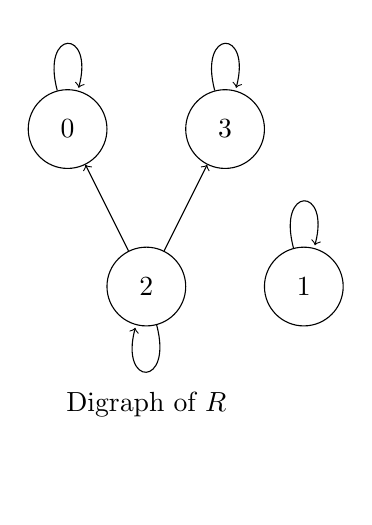
\begin{tikzpicture}[scale=1, every node/.style={circle,draw,minimum size=1cm}]
            \node (0) at (0,2) {0};
            \node (3) at (2,2) {3};
            \node (2) at (1,0) {2};
            \node (1) at (3,0) {1};
            % Reflexive loops
            \draw[->] (0) edge[loop above] ();
            \draw[->] (1) edge[loop above] ();
            \draw[->] (2) edge[loop below] ();
            \draw[->] (3) edge[loop above] ();
            % Edges
            \draw[->] (2) -- (0);
            \draw[->] (2) -- (3);
            % Label
            \node[draw=none,fill=none] at (1,-1.5) {Digraph of $R$};
          \end{tikzpicture}
        \end{minipage}
        \hfill
        % Hasse diagram for the relation R
        \begin{minipage}{0.45\textwidth}
          \centering
          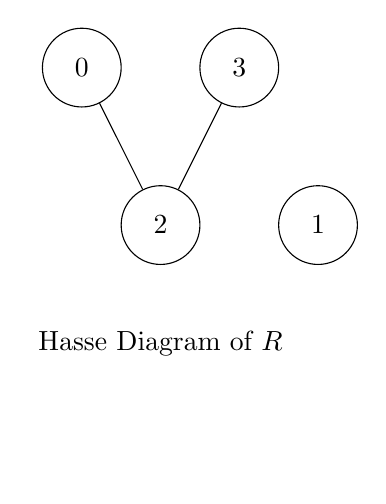
\begin{tikzpicture}[scale=1, every node/.style={circle,draw,minimum size=1cm}]
            \node (0) at (0,2) {0};
            \node (3) at (2,2) {3};
            \node (2) at (1,0) {2};
            \node (1) at (3,0) {1};
            % Covering relations (no loops)
            \draw (2) -- (0);
            \draw (2) -- (3);
            % Label
            \node[draw=none,fill=none] at (1,-1.5) {Hasse Diagram of $R$};
          \end{tikzpicture}
        \end{minipage}
      \end{center}
    \end{subanswer}
  \end{enumerate}

    \item Draw the Hasse diagram for the relation $R = \{(1,1), (1,2), (1,3), (2,2), (2,3), (3,3)\}$ on the set $S = \{1, 2, 3\}$.
    \begin{subanswer}
      The given relation $R$ is a partial ordering on $S$ 
      since it satisfies reflexivity, antisymmetry, and transitivity.
      Thus, it is possible to draw the Hasse diagram for the relation $R$ on the set $S$ as follows.
      \begin{center}
        % Digraph for the relation R
        \begin{minipage}{0.45\textwidth}
          \centering
          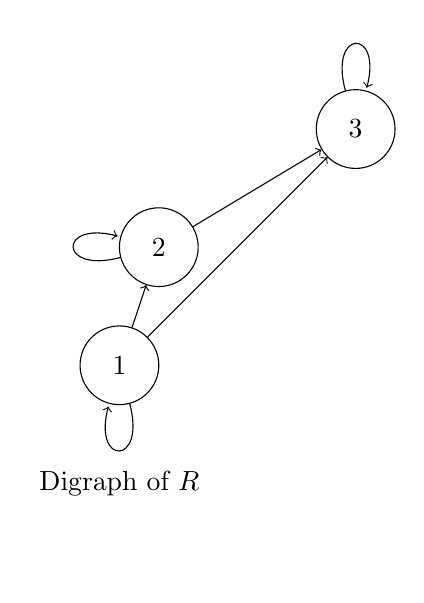
\begin{tikzpicture}[scale=1, every node/.style={circle,draw,minimum size=1cm}]
            \node (1) at (0,0) {1};
            \node (2) at (0.5,1.5) {2};
            \node (3) at (3,3) {3};
            % Reflexive loops
            \draw[->] (1) edge[loop below] ();
            \draw[->] (2) edge[loop left] ();
            \draw[->] (3) edge[loop above] ();
            % Chain edges
            \draw[->] (1) -- (2);
            \draw[->] (2) -- (3);
            \draw[->] (1) -- (3);
            % Label
            \node[draw=none,fill=none] at (0,-1.5) {Digraph of $R$};
          \end{tikzpicture}
        \end{minipage}
        \hfill
        % Hasse diagram for the relation R
        \begin{minipage}{0.45\textwidth}
          \centering
          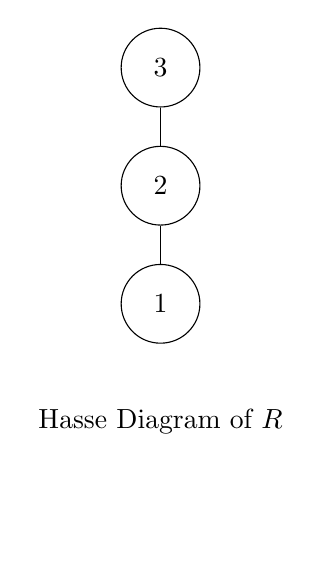
\begin{tikzpicture}[scale=1, every node/.style={circle,draw,minimum size=1cm}]
            \node (1) at (0,0) {1};
            \node (2) at (0,1.5) {2};
            \node (3) at (0,3) {3};
            % Chain edges (no loops)
            \draw (1) -- (2);
            \draw (2) -- (3);
            % Label
            \node[draw=none,fill=none] at (0,-1.5) {Hasse Diagram of $R$};
          \end{tikzpicture}
        \end{minipage}
      \end{center}
    \end{subanswer}

  \newpage
  \item Show that if the poset $(S, R)$ is a lattice, then the dual poset $\left(S, R^{-1}\right)$ is also a lattice.
  \begin{define}{Dual Poset}[def:dual-poset][red]
    Let $(S, \preccurlyeq)$ be a partially ordered set (poset). 
    The \textbf{dual poset} is the pair $(S, \preccurlyeq^{-1})$, 
    where $\preccurlyeq^{-1}$ is the inverse relation of $\preccurlyeq$. 
    For any elements $a, b \in S$ such that
    \[
      a \preccurlyeq^{-1} b \IFF b \preccurlyeq a
    \]
    \textbf{Note}: $\succcurlyeq$ is used to denote the inverse relation $\preccurlyeq^{-1}$, so the dual poset is written as $(S, \succcurlyeq)$.
  \end{define}
  \begin{define}{Lattice}[def:lattice][red]
    Let $(S, R)$ be a poset. $(S, R)$ is a \textbf{lattice} if and only if for every $a, b \in S$:
    \begin{itemize}
      \item There exists a unique \textbf{least upper bound} (join), denoted $(a \JOIN b)$, such that:
        \begin{enumerate}
          \item \textbf{Upper Bound}: $\relation{a}{(a \JOIN b)}$ and $\relation{b}{(a \JOIN b)}$,
          \item \textbf{Uniqueness (Supremum)}: For any $u \in S$, if $\relation{a}{u}$ and $\relation{b}{u}$, then $\relation{(a \JOIN b)}{u}$.
        \end{enumerate}
      \item There exists a unique \textbf{greatest lower bound} (meet), denoted $(a \MEET b)$, such that:
        \begin{enumerate}
          \item \textbf{Unique Lower Bound}: $\relation{(a \MEET b)}{a}$ and $\relation{(a \MEET b)}{b}$.
          \item \textbf{Uniqueness (Infimum)}: For any $l \in S$, if $\relation{l}{a}$ and $\relation{l}{b}$, then $\relation{l}{(a \MEET b)}$.
        \end{enumerate}
    \end{itemize}
  \end{define}
  \begin{subprove}
    Let $(S, R)$ be a lattice for the sake of direct proof.
    By definition of \nameref{def:lattice}, for every $a, b \in S$,
    there exists supremum and infimum with respect to $R$.
    By definition of \nameref{def:dual-poset},
    \begin{itemize}
      \item Consider the infimum, $a \MEET b$ with respect to $R$.
      By definition, for any $a, b \in S$,
      \begin{enumerate}
        \item $\relation{(a \MEET b)}{a}$ and $\relation{(a \MEET b)}{b}$.
        By definition of \nameref{def:dual-poset}, 
        it follows that $\relationinv{a}{(a \MEET b)}$ and $\relationinv{b}{(a \MEET b)}$.
        Thus, $a \MEET b$ is an upper bound of $a$ and $b$ with respect to $R^{-1}$.
        \item $\relation{l}{a}$ and $\relation{l}{b}$, 
        then $\relation{l}{(a \MEET b)}$ for any $l \in S$.
        By definition of \nameref{def:dual-poset}, it follows that 
        if $\relationinv{a}{l}$ and $\relationinv{b}{l}$, then $\relationinv{(a \MEET b)}{l}$.
        Thus, by definition of supremum, $a \MEET b$ is the least upper bound of $a$ and $b$ 
        with respect to $R^{-1}$, denoted by $a \JOIN' b = a \MEET b$.
      \end{enumerate}
      Therefore, there exists the supremum with respect to $R^{-1}$.
      \item Consider the supremum, $a \JOIN b$ with respect to $R$.
      By definition, for any $a, b \in S$,
      \begin{enumerate}
        \item $\relation{a}{(a \JOIN b)}$ and $\relation{b}{(a \JOIN b)}$.
        By definition of \nameref{def:dual-poset}, 
        it follows that $\relationinv{(a \JOIN b)}{a}$ and $\relationinv{(a \JOIN b)}{b}$.
        Thus, $a \JOIN b$ is a lower bound of $a$ and $b$ with respect to $R^{-1}$.
        \item $\relation{a}{u}$ and $\relation{b}{u}$, 
        then $\relation{(a \JOIN b)}{u}$ for any $u \in S$.
        By definition of \nameref{def:dual-poset}, it follows that 
        if $\relationinv{u}{a}$ and $\relationinv{u}{b}$, then $\relationinv{u}{(a \JOIN b)}$.
        Thus, by definition of infimum, $a \JOIN b$ is the greatest lower bound of $a$ and $b$ 
        with respect to $R^{-1}$, denoted by $a \MEET' b = a \JOIN b$.
      \end{enumerate}
      Therefore, there exists the infimum with respect to $R^{-1}$.
    \end{itemize}
    Since both supremum and infimum exist with respect to $R^{-1}$ for every $a, b \in S$,
    it follows that $(S, R^{-1})$ is a poset by definition of \nameref{def:poset}.
    Therefore, by direct proof, the dual poset $\left(S, R^{-1}\right)$ is also a lattice by definition of \nameref{def:lattice}.
  \end{subprove}

  \newpage
  \item Draw the \textbf{Hasse diagrams} for three lattice (partially ordered set) examples.
  \begin{define}{Hasse Diagram}[def:hasse-diagram][red]
    Let $(P, \preceq)$ be a finite partially ordered set (poset).  
    The \textbf{Hasse diagram} of $(P, \preceq)$ is a 
    \textbf{directed graph} $G = (P, E)$ with \textbf{upward} directed edges defined as follows.
    \begin{itemize}
      \item The \textbf{vertex set} is
        \[
          V = P.
        \]
      \item The \textbf{edge set} is
        \[
          E = \{\, (a, b) \in P \times P \mid a \prec b 
          \text{ and there does not exists } c \in P \text{ such that } a \prec c \prec b \,\},
        \]
        where $a \prec b$ denotes that $a \preceq b$ and $a \neq b$.
    \end{itemize}
  \end{define}
  \begin{subanswer}
    Here are three examples of lattices.\\
    \begin{minipage}{0.30\textwidth}
      \centering
      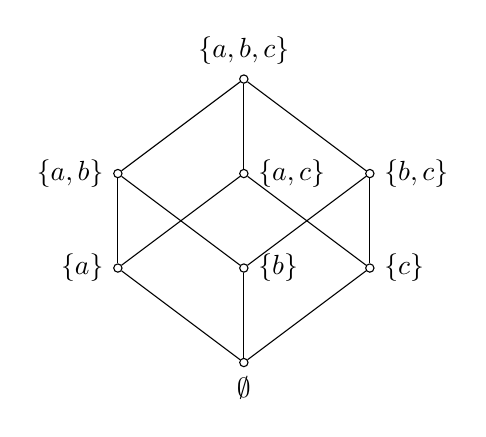
\begin{tikzpicture}[scale=0.8]
        % Nodes (bottom to top)
        \node (empty) at (0,0) [circle, draw, inner sep=0pt, minimum size=3pt, label=below:{$\emptyset$}] {};
        \node (a) at (-2,1.5) [circle, draw, inner sep=0pt, minimum size=3pt, label=left:{$\{a\}$}] {};
        \node (b) at (0,1.5) [circle, draw, inner sep=0pt, minimum size=3pt, label=right:{$\{b\}$}] {};
        \node (c) at (2,1.5) [circle, draw, inner sep=0pt, minimum size=3pt, label=right:{$\{c\}$}] {};

        \node (ab) at (-2,3) [circle, draw, inner sep=0pt, minimum size=3pt, label=left:{$\{a,b\}$}] {};
        \node (ac) at (0,3) [circle, draw, inner sep=0pt, minimum size=3pt, label=right:{$\{a,c\}$}] {};
        \node (bc) at (2,3) [circle, draw, inner sep=0pt, minimum size=3pt, label=right:{$\{b,c\}$}] {};

        \node (abc) at (0,4.5) [circle, draw, inner sep=0pt, minimum size=3pt, label=above:{$\{a,b,c\}$}] {};

        % Edges (bottom to singletons)
        \draw (empty) -- (a);
        \draw (empty) -- (b);
        \draw (empty) -- (c);

        % Edges (singletons to pairs)
        \draw (a) -- (ab);
        \draw (a) -- (ac);
        \draw (b) -- (ab);
        \draw (b) -- (bc);
        \draw (c) -- (ac);
        \draw (c) -- (bc);

        % Edges (pairs to top)
        \draw (ab) -- (abc);
        \draw (ac) -- (abc);
        \draw (bc) -- (abc);
      \end{tikzpicture}
      \parbox{3cm}{\centering $(\opP(\{a,b,c\}), \subseteq)$}
    \end{minipage}
    \hfill
    \begin{minipage}{0.30\textwidth}
      \centering
      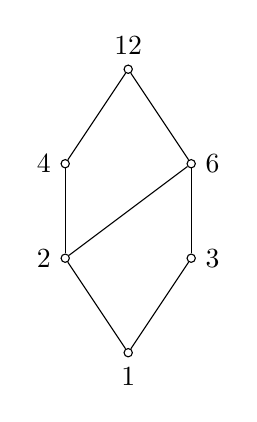
\begin{tikzpicture}[scale=0.8]
        % Nodes
        \node (1)  at (0,0) [circle, draw, inner sep=0pt, minimum size=3pt, label=below:$1$] {};
        \node (2)  at (-1,1.5) [circle, draw, inner sep=0pt, minimum size=3pt, label=left:$2$] {};
        \node (3)  at (1,1.5) [circle, draw, inner sep=0pt, minimum size=3pt, label=right:$3$] {};
        \node (4)  at (-1,3) [circle, draw, inner sep=0pt, minimum size=3pt, label=left:$4$] {};
        \node (6)  at (1,3) [circle, draw, inner sep=0pt, minimum size=3pt, label=right:$6$] {};
        \node (12) at (0,4.5) [circle, draw, inner sep=0pt, minimum size=3pt, label=above:$12$] {};

        % Edges
        \draw (1) -- (2);
        \draw (1) -- (3);
        \draw (2) -- (4);
        \draw (2) -- (6);
        \draw (3) -- (6);
        \draw (4) -- (12);
        \draw (6) -- (12);
      \end{tikzpicture}
      \parbox{3cm}{\centering $(D_{12} (\text{divisors}), \mid)$}
    \end{minipage}
    \hfill
    \begin{minipage}{0.30\textwidth}
      \centering
        \begin{tikzpicture}[scale=1]
          % Nodes
          \node (bot) at (0,0) [circle, draw, inner sep=0pt, minimum size=3pt, label=below:{$p \AND q$}] {};
          \node (p)   at (-1.2,1.5) [circle, draw, inner sep=0pt, minimum size=3pt, label=left:{$p$}] {};
          \node (q)   at (1.2,1.5) [circle, draw, inner sep=0pt, minimum size=3pt, label=right:{$q$}] {};
          \node (pq)  at (0,3) [circle, draw, inner sep=0pt, minimum size=3pt, label=above:{$p \OR q$}] {};

          % Edges
          \draw (bot) -- (p);
          \draw (bot) -- (q);
          \draw (p) -- (pq);
          \draw (q) -- (pq);
        \end{tikzpicture}
        \parbox{4cm}{\centering $(\{p \AND q, p, q, p \OR q\}, \THEN)$}
    \end{minipage}
  \end{subanswer}


  \item For the lattice of all divisors of 60, ordered by divisibility, find the join and meet of 12 and 15.
  \begin{subanswer}
    The divisors of 60 are $S = \{1, 2, 3, 4, 5, 6, 10, 12, 15, 20, 30, 60\}$.
    The Hasse diagram for the lattice of all divisors of 60 is as follows.
    \begin{center}
      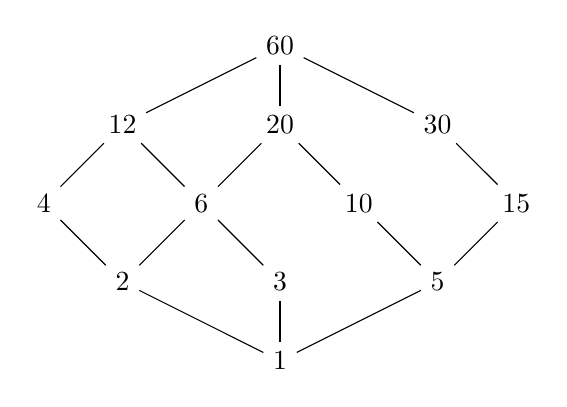
\begin{tikzpicture}[scale=1.0]
        \node (1) at (0,0) {1};
        \node (2) at (-2,1) {2};
        \node (3) at (0,1) {3};
        \node (4) at (2,1) {5};
        \node (5) at (-3,2) {4};
        \node (6) at (-1,2) {6};
        \node (7) at (1,2) {10};
        \node (8) at (3,2) {15};
        \node (9) at (-2,3) {12};
        \node (10) at (0,3) {20};
        \node (11) at (2,3) {30};
        \node (12) at (0,4) {60};

        \draw (1) -- (2);
        \draw (1) -- (3);
        \draw (1) -- (4);
        \draw (2) -- (5);
        \draw (2) -- (6);
        \draw (3) -- (6);
        \draw (4) -- (7);
        \draw (4) -- (8);
        \draw (5) -- (9);
        \draw (6) -- (9);
        \draw (6) -- (10);
        \draw (7) -- (10);
        \draw (8) -- (11);
        \draw (9) -- (12);
        \draw (10) -- (12);
        \draw (11) -- (12);
      \end{tikzpicture}
    \end{center}
    The supremum (join) and infimum (meet) can be found as follows.
    $$12 \JOIN 15 = 60 \text{ and } 12 \MEET 15 = 3$$
  \end{subanswer}

  \newpage
  

  \item Draw the \textbf{Hasse diagrams} for three chain (linearly ordered set) examples.
  \begin{subanswer}
    Here are three examples of chains (linearly ordered sets).\\
    \begin{minipage}{0.30\textwidth}
      \centering
      \begin{tikzpicture}[scale=1]
        % Nodes (bottom to top)
        \node (dots_b) at (0,-0.5) {$\vdots$};
        \node (n1) at (0,0) [circle, draw, inner sep=0pt, minimum size=3pt, label=right:$-1$] {};
        \node (0)  at (0,1) [circle, draw, inner sep=0pt, minimum size=3pt, label=right:$0$] {};
        \node (1)  at (0,2) [circle, draw, inner sep=0pt, minimum size=3pt, label=right:$1$] {};
        \node (dots_t) at (0,2.5) {$\vdots$};
        % Edges
        \draw (dots_b) -- (n1) -- (0) -- (1) -- (dots_t);
      \end{tikzpicture}
      \parbox{3cm}{\centering $(\setZ, \leq)$}
    \end{minipage}
    \hfill
    \begin{minipage}{0.30\textwidth}
      \centering
      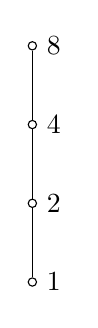
\begin{tikzpicture}[scale=1]
        % Nodes (bottom to top)
        \node (1) at (0,0) [circle, draw, inner sep=0pt, minimum size=3pt, label=right:$1$] {};
        \node (2) at (0,1) [circle, draw, inner sep=0pt, minimum size=3pt, label=right:$2$] {};
        \node (4) at (0,2) [circle, draw, inner sep=0pt, minimum size=3pt, label=right:$4$] {};
        \node (8) at (0,3) [circle, draw, inner sep=0pt, minimum size=3pt, label=right:$8$] {};
        % Edges
        \draw (1) -- (2) -- (4) -- (8);
      \end{tikzpicture}
      \parbox{4cm}{\centering $(D_8 (\text{divisors}), \mid)$}
    \end{minipage}
    \hfill
    \begin{minipage}{0.30\textwidth}
      \centering
      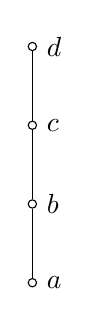
\begin{tikzpicture}[scale=1]
        % Nodes (bottom to top)
        \node (a) at (0,0) [circle, draw, inner sep=0pt, minimum size=3pt, label=right:$a$] {};
        \node (b) at (0,1) [circle, draw, inner sep=0pt, minimum size=3pt, label=right:$b$] {};
        \node (c) at (0,2) [circle, draw, inner sep=0pt, minimum size=3pt, label=right:$c$] {};
        \node (d) at (0,3) [circle, draw, inner sep=0pt, minimum size=3pt, label=right:$d$] {};
        % Edges
        \draw (a) -- (b) -- (c) -- (d);
      \end{tikzpicture}
      \parbox{3cm}{\centering $(\text{Alphabet}, <)$}
    \end{minipage}
  \end{subanswer}


  \item Prove that every chain (also known as a totally ordered set) is a lattice.
  \begin{define}{Chain (Linearly Ordered Set)}[def:chain][red]
    Let $(S, R)$ be a poset. $(S, R)$ is called a \textbf{chain} (or \textbf{linearly ordered set}) if for all $a, b \in S$, $R$ is total; that is,
    \[
      \forall a, b \in S,\; (a, b) \in R \text{ or } (b, a) \in R.
    \]
    Equivalently, every pair of elements in $S$ is comparable under $R$.
  \end{define}
  \begin{subprove}
    Let $(S, R)$ be a chain for the sake of direct proof.
    By definition of \nameref{def:chain}, for all $a, b \in S$, either $\relation{a}{b}$ or $\relation{b}{a}$.
    Let $a, b \in S$ be arbitrary. Then, by cases as follows,
    \begin{itemize}
      \item If $\relation{a}{b}$, then $b$ is an upper bound of $a$ and $b$ with respect to $R$.
      Also, for every upper bound $d$ of $a$ and $b$, 
      since either $\relation{b}{d}$ or $\relation{d}{b}$, 
      it follows that $\relation{b}{d}$.
      Thus, by definition of infimum, 
      $b$ is the least upper bound of $a$ and $b$, denoted by $a \JOIN b = b$.
      Similarly, $a$ is the greatest lower bound of $a$ and $b$, denoted by $a \MEET b = a$.
      \item If $\relation{b}{a}$, then by similar reasoning as above, 
      it follows that $a$ is the least upper bound of $a$ and $b$, denoted by $a \JOIN b = a$
      and $b$ is the greatest lower bound of $a$ and $b$, denoted by $a \MEET b = b$.
    \end{itemize}
    Therefore, by direct proof, every chain is a lattice by definition of \nameref{def:lattice}.
  \end{subprove}


  \newpage
  \item Give an example of an infinite lattice (and justify your answer) with: 
  \begin{enumerate}
    \item neither a least nor a greatest element
    \begin{subanswer}
      Let $S = \set{\ldots, -3, -2, -1, 0, 1, 2, 3, \ldots}$ be the set of all integers and let $R$ be the relation defined by the usual order $\leq$ on $S$.
      Then, $(S, R)$ is a poset since $\leq$ is reflexive, antisymmetric, and transitive.
      Also, for all $a, b \in S$, both the least upper bound (join) and the greatest lower bound (meet) of $a$ and $b$ exist in $S$.
      Specifically, for any two integers $a$ and $b$, 
      \begin{enumerate}
        \item the least upper bound (join) is given by $\max(a,b)$
        \item the greatest lower bound (meet) is given by $\min(a,b)$
      \end{enumerate}
      which are both integers. Thus, $(S, R)$ is a lattice by definition of \nameref{def:lattice}.\proofstep
      However, $(S, R)$ has neither a least element nor a greatest element since for any integer $n$, 
      there exists an integer $m = n - 1$ such that $m < n$ (hence no least element), 
      and there exists an integer $p = n + 1$ such that $p > n$ (hence no greatest element).\proofstep
      Therefore, by example and justification, $(S, R)$ is an infinite lattice with neither a least nor a greatest element.
    \end{subanswer}
    \item a least but not a greatest element
    \begin{subanswer}
      Let $S = \set{0, 1, 2, 3, \ldots}$ be the set of all nonnegative integers and let $R$ be the relation defined by the usual order $\leq$ on $S$.
      Then, $(S, R)$ is a poset since $\leq$ is reflexive, antisymmetric, and transitive.
      Also, for all $a, b \in S$, both the least upper bound (join) and the greatest lower bound (meet) of $a$ and $b$ exist in $S$.
      Specifically, for any two nonnegative integers $a$ and $b$, 
      \begin{enumerate}
        \item the least upper bound (join) is given by $\max(a,b)$
        \item the greatest lower bound (meet) is given by $\min(a,b)$
      \end{enumerate}
      which are both nonnegative integers. Thus, $(S, R)$ is a lattice by definition of \nameref{def:lattice}.\proofstep
      Moreover, $(S, R)$ has a least element $0$ since for any nonnegative integer $n$, $0 \leq n$.
      However, $(S, R)$ has no greatest element since for any nonnegative integer $n$, 
      there exists a nonnegative integer $m = n + 1$ such that $m > n$.\proofstep
      Therefore, by example and justification, $(S, R)$ is an infinite lattice with a least but not a greatest element.
    \end{subanswer}
    \item a greatest but not a least element
    \begin{subanswer}
      Let $S = \set{\ldots, -3, -2, -1, 0}$ be the set of all nonpositive integers and let $R$ be the relation defined by the usual order $\leq$ on $S$.
      Then, $(S, R)$ is a poset since $\leq$ is reflexive, antisymmetric, and transitive.
      Also, for all $a, b \in S$, both the least upper bound (join) and the greatest lower bound (meet) of $a$ and $b$ exist in $S$.
      Specifically, for any two nonpositive integers $a$ and $b$, 
      \begin{enumerate}
        \item the least upper bound (join) is given by $\max(a,b)$
        \item the greatest lower bound (meet) is given by $\min(a,b)$
      \end{enumerate}
      which are both nonpositive integers. Thus, $(S, R)$ is a lattice by definition of \nameref{def:lattice}.\proofstep
      Moreover, $(S, R)$ has a greatest element $0$ since for any nonpositive integer $n$, $n \leq 0$.
      However, $(S, R)$ has no least element since for any nonpositive integer $n$, 
      there exists a nonpositive integer $m = n - 1$ such that $m < n$.\proofstep
      Therefore, by example and justification, $(S, R)$ is an infinite lattice with a greatest but not a least element.
    \end{subanswer}
    \item both a least and a greatest element
    \begin{subanswer}
      Let $S = \set{0}$ be the set containing only the single element $0$ and let $R$ be the relation defined by the usual order $\leq$ on $S$.
      Then, $(S, R)$ is a poset since $\leq$ is reflexive, antisymmetric, and transitive.
      Also, for all $a, b \in S$, both the least upper bound (join) and the greatest lower bound (meet) of $a$ and $b$ exist in $S$.
      Specifically, for any two elements $a$ and $b$ in $S$, 
      \begin{enumerate}
        \item the least upper bound (join) is given by $\max(a,b)$
        \item the greatest lower bound (meet) is given by $\min(a,b)$
      \end{enumerate}
      which are both equal to $0$. Thus, $(S, R)$ is a lattice by definition of \nameref{def:lattice}.\proofstep
      Moreover, $(S, R)$ has a least element $0$ since $0 \leq 0$.
      Additionally, $(S, R)$ has a greatest element $0$ since $0 \geq 0$.\proofstep
      Therefore, by example and justification, $(S, R)$ is a finite lattice with both a least and a greatest element.
    \end{subanswer}
  \end{enumerate}








\end{enumerate}








































\newpage\handout[true]
{\textsc{Math 2106-B: Foundations of Mathematical Proof}}{Fall 2025}
{Homework 6: Groups and Subgroups}
{\textit{Prof.} \href{https://ceheitsch.github.io/webpage/}{Dr. Christine Heitsch}}{Due Date: October 23, 2025}
{Math 2106-B: HW6}
{\large
  \noindent
  \textbf{Name:} \HandoutAuthor \smallskip \\

  \noindent
  \textbf{GTID:} 903743506 \smallskip \\

  \noindent
  %%% List anyone with whom you discussed the problems
  \textbf{Collaborators:} None. This material reflects independent preparation. \smallskip \\

  \noindent
  %%% List all resources used OTHER than the textbook, lecture notes, 
  %%% webwork problems, ICA questions, and previous homework assignments.
  \textbf{Outside resources:} This work was informed by MATH 2106 course materials 
  (ICAs: in-class activities and WebWork contents) from \HandoutInstitution\ (the course textbook is 
  Chartrand \parencite{chartrand_mathematical_2018}).   
  Outside references specifically include
  textbooks written by 
  Grimaldi \parencite{grimaldi_discrete_2004} (used in MATH 3012) and 
  Rosen \parencite{rosen_discrete_2019} (used in CS 2050). \smallskip \\

  \noindent
  \textbf{Notice}: The answers contain cross-references throughout this document as clickable hyperlinks in most PDF viewers. However, the Gradescope PDF view might not support clickable hyperlinks.
}
\printbibliography[
  heading=bibintoc,   
  title={References}     % change “References” text if needed
]
% `heading=bibnumbered` if you prefer it numbered chapter (in \tableofcontents)
% `heading=bibintoc`    if you prefer it unnumbered but still in the ToC
\newpage
% \printbibliography[
  heading=bibintoc,   
  title={References}     % change “References” text if needed
]
% `heading=bibnumbered` if you prefer it numbered chapter (in \tableofcontents)
% `heading=bibintoc`    if you prefer it unnumbered but still in the ToC\newpage
% The following table presents the standard logical equivalences from these sources together with 
the author's own (or the student, myself, Jaehoon Song) clarifications and labels where applicable.


\begin{table}[h!]
  \centering
  \renewcommand{\arraystretch}{1.2}
  \setlength{\tabcolsep}{8pt}
  \begin{tabular}{|p{5.0cm}|p{5.0cm}|p{5.2cm}|}
    \hline
    \rowcolor[HTML]{E0E0E0}
    \multicolumn{2}{|l|}{\textbf{Logical Equivalences}} & \textbf{Name} \\
    \hline
    $\,p \AND q \equiv q \AND p$ & $\,p \OR q \equiv q \OR p$ & Commutative Law \\
    \hline
    $\, (p \AND q) \AND r \equiv p \AND (q \AND r)$ & $\, (p \OR q) \OR r \equiv p \OR (q \OR r)$ & Associative Law \\
    \hline
    $\,p \AND (q \OR r) \equiv (p \AND q) \OR (p \AND r)$ & $\,p \OR (q \AND r) \equiv (p \OR q) \AND (p \OR r)$ & Distributive Law \\
    \hline
    $\,\overline{p \AND q} \equiv \sNOT{p} \OR \sNOT{q}$ & $\,\overline{p \OR q} \equiv \sNOT{p} \AND \sNOT{q}$ & DeMorgan's Law \\
    \hline
    \multicolumn{2}{|l|}{$\,\overline{\overline{p}} \equiv p$} & Double Negation law \\
    \hline
    $\,p \AND \boldsymbol{T} \equiv p$ & $\,p \OR \boldsymbol{F} \equiv p$ & Identity Law \\
    \hline
    $\,p \OR \boldsymbol{T} \equiv \boldsymbol{T}$ & $\,p \AND \boldsymbol{F} \equiv \boldsymbol{F}$ & Domination Law \\
    \hline
    $\,p \AND p \equiv p$ & $\,p \OR p \equiv p$ & Idempotent Law \\
    \hline
    \multicolumn{2}{|l|}{$\,p \THEN q \equiv \sNOT{p} \OR q$} & Implication Equivalence \\
    \hline
    \multicolumn{2}{|l|}{$\,\overline{p \THEN q} \equiv p \AND \sNOT{q}$} & Negation of Implication \\
    \hline
    \multicolumn{2}{|l|}{$\,p \THEN q \equiv \sNOT{q} \THEN \sNOT{p}$} & Contrapositive Equivalence \\
    \hline
    \multicolumn{2}{|l|}{$\,p \OR \sNOT{p} \equiv \boldsymbol{T}$} & Law of Tautology \\
    \hline
    \multicolumn{2}{|l|}{$\,p \AND \sNOT{p} \equiv \boldsymbol{F}$} & Law of Contradiction \\
    \hline
  \end{tabular}
\end{table}\newpage
% 
The following definitions are presented from standard mathematical sources (\textbf{Sets}).
Clarifications and labels have been added where applicable.

\begin{define}{Basic Set Concepts}\phantomsection\label{def:basic-set-concepts} % \hyperref[def:basic-set-concepts]{YOUR_CONTEXT}
  \begin{enumerate}
    \item \textbf{Universal Set:} A universal set $\setUNIV$ is a
    set that contains all objects under consideration in a particular context or problem.
    \item \textbf{Empty Set:} The empty set, denoted $\setNULL$,
    is the unique set that contains no elements.
    \item \textbf{Subset:} Let $A$ and $B$ be sets. $A$ is a
    subset of $B$ ($A \subseteq B$) if (and only if)
    for all $x \in A$, $x \in B$.
    \item \textbf{Set Equality:} Let $A$ and $B$ be sets. The sets $A$ and $B$ are
    equal ($A = B$) if $A \subseteq B$ and $B \subseteq A$.
    \item \textbf{Power Set:} Let $A$ be a set. The power set of $A$, denoted $\sPOWER{A}$ or $2^A$,
    is the set of all subsets of $A$. That is, $\mathcal{P}(A) = \{S\in\setUNIV : S \subseteq A\}$.
  \end{enumerate}
\end{define}
The following definitions extend the understanding of set operations
and properties.


\begin{define}{Set Operations}\phantomsection\label{def:set-operations} % \hyperref[def:set-operations]{YOUR_CONTEXT}
  \begin{enumerate}
    \item \textbf{Complementary Set:} Let $A$ be a subset of the universal set $\setUNIV$.
    The complement of $A$, denoted $A^c$ or $\overline{A}$, is the set of all elements
    in $\setUNIV$ that are not in $A$. That is, $A^c = \{x \in \setUNIV : x \notin A\}$.
    \item \textbf{Union:} Let $A$ and $B$ be sets. The union of $A$ and $B$,
    denoted $A \cup B$, is the set of all elements that are in $A$, or in $B$, or in both.
    That is, $A \cup B = \{x : x \in A \lor x \in B\}$.
    \item \textbf{Intersection:} Let $A$ and $B$ be sets. The intersection of $A$ and $B$,
    denoted $A \cap B$, is the set of all elements that are in both $A$ and $B$.
    That is, $A \cap B = \{x : x \in A \land x \in B\}$.
    \item \textbf{Set Difference:} Let $A$, $B$ be subsets of a universal set $\setUNIV$.
    The set difference $A \sMINUS B$ is defined to be the set
    $\{ x \in \setUNIV \LDIV x \in A \text{ and } x \notin B\}$. \vspace*{10px}\\
    \textit{It is sometimes called the relative complement of $B$ in $A$,
    and denoted in the textbook as $A - B$.}
    \item \textbf{Cartesian Product:} Let $A$ and $B$ be sets. The Cartesian product of
    $A$ and $B$, denoted $A \sTIMES B$, is the set consisting of all ordered pairs:
    \[
    A \sTIMES B = \{(a, b) \LDIV a \in A, b \in B\}.
    \]
  \end{enumerate}
\end{define}


\newpage

The following claims are given in the reference as well. Let $A,B\in U$, a universal set.


\begin{claim}{Subset of Union: $A \subseteq \sOR{A}{B}$}\phantomsection\label{claim:subset-union} % \hyperref[claim:subset-union]{YOUR_CONTEXT}
  \begin{subprove}[bluecolor]
      Let $x\in U$, assume $x\in A$. Then the statement \inlinequote{$x\in A$ or $x\in B$} is true.
      Hence, by the definition, $\sOR{A}{B}=\{x\in U\LDIV x\in A$ or $x\in B\}$, $x\in \sOR{A}{B}$.
      Thus, $A \subseteq \sOR{A}{B}$.
  \end{subprove}
\end{claim}

\begin{claim}{Empty Subset: $\setNULL \subseteq A$}\phantomsection\label{claim:empty-subset} % \hyperref[claim:empty-subset]{YOUR_CONTEXT}
  \begin{subprove}[bluecolor]
      Let $x\in U$, assume $x\in \setNULL$. But there are no elements in $\setNULL$, so
      $x\in \setNULL$ is false. Since the premise is false, the implication if $x\in \setNULL$,
      then $x\in A$ is true. Thus, $\setNULL \subseteq A$ by definition of \hyperref[def:basic-set-concepts]{subsets}.
  \end{subprove}
\end{claim}

\begin{claim}{Subset as Equality: $\sOR{A}{B}=A$ if and only if $B\subseteq A$}\phantomsection\label{claim:subset-equality} % \hyperref[claim:subset-equality]{YOUR_CONTEXT}
  \begin{subprove}[bluecolor]
      Let $x\in U$, first, we assume $B\subseteq A$, we have already shown
      $A \subseteq \sOR{A}{B}$ by the claim, \hyperref[claim:subset-union]{Subset of Union}. 
      To show $\sOR{A}{B} \subseteq A$, assume $x\in \sOR{A}{B}$.
      By definition, $x\in A$ or $x\in B$. Considering $x\in B$ and assumption
      $B \subseteq A$, $x\in B$ implies $x\in A$. Thus, $\sOR{A}{B} \subseteq A$.
      Hence, if $B\subseteq A$, then $\sOR{A}{B} = A$. \vspace*{10px}\\
      Now, we assume $\sOR{A}{B}=A$. To show $B\subseteq A$, we now assume $x\in B$. Since $x\in B$, by definition
      of union, $x\in \sOR{A}{B} = A$. Therefore, $B\subseteq A$.
  \end{subprove}
\end{claim}


%%%%%%%%%%%%%%%%%%% 9/8/25

Let $\setUNIV$ be a set. 
\begin{claim}{ICA6}\phantomsection\label{claim:ica6} % \hyperref[claim:ica6]{YOUR_CONTEXT}
  For all $A,B\in\setUNIV$, $$A\sTIMES B =\setNULL\THEN \group{A=\setNULL\OR B=\setNULL}$$
  \begin{subprove}[bluecolor]
    Let $A,B\in\setUNIV$. We prove $A\sTIMES B=\setNULL$. Assume it is not the case that 
    $A=\setNULL$ or $B=\setNULL$. Thus, we have $A=\setNULL$ and $B=\setNULL$. 
    Since $A\ne\setNULL$ by assumption, there exists an element $a\in A$. Likewise, there 
    is some $b\in B$ since $B\ne\setNULL$. Thus, $\group{a,b}\in\sBUILD{(x,y)}{x\in A,y\in B}$ 
    by definition. But then, $A\sTIMES B\ne\setNULL$ by definition. Hence, the claim holds. 
  \end{subprove}
\end{claim}


\begin{define}{Relatively Prime Integers (Coprime)}\phantomsection\label{def:relatively-prime} % \hyperref[def:relatively-prime]{YOUR_CONTEXT}
  Let $x,y \in \mathbb{Z}$. The integers $x$ and $y$ are said to be
  \textbf{relatively prime} if and only if
  $\gcd(x,y) = 1$.
\end{define}
\newpage
% The following definitions and axioms are presented from standard mathematical sources (\textbf{Number Theory}) together with the author's own (or the student, myself, Jaehoon Song) clarifications and labels where applicable.

\begin{define}{Integers}[def:integers][red]
  $\setZ$: the set of all integers
\end{define}

\begin{define}{Rational Numbers}[def:rational-numbers][red]
  $\setQ$: the set of all rational numbers
\end{define}

\begin{define}{Real Numbers}[def:real-numbers][red]
  $\setR$: the set of all real numbers
\end{define}

\begin{define}{Natural Numbers}[def:natural-numbers][red]
  $\setN$ or $\setZ_{>0}$: the set of all natural numbers which are the set of positive integers (not including $0$)
\end{define}

\begin{define}{Positive Real Numbers}[def:positive-real-numbers][red]
  $\setR_{>0}$: the set of all positive real numbers
\end{define}

\begin{define}{Non-negative Real Numbers}[def:non-negative-real-numbers][red]
  $\setR_{\geq 0}$: the set of all non-negative real numbers
\end{define}


\newpage

The following definitions and claims extend the understanding of integers.

Here are the ICA2 Definitions and Axioms as follows.

\begin{define}{Even Integer}[def:even-integer][red]
  An integer $n$ is \underbar{even} if there exists 
  (existential quantification logic $\exists$) an integer $k$ such that
  \[
  n = 2k.
  \]
\end{define}

\begin{define}{Odd Integer}[def:odd-integer][red]
  An integer $n$ is \underbar{odd} if 
  there exists some integer $k$ such that
  \[
  n = 2k + 1.
  \]
\end{define}

\begin{define}{Closure under Addition}[def:closure-addition][red]
  The sum of two integers is again an 
  integer. (Closure under addition)
\end{define}

\begin{define}{Closure under Multiplication}[def:closure-multiplication][red]
  The product of two integers is again 
  an integer. (Closure under multiplication)
\end{define}

\begin{define}{Odd if and only if Not Even}[def:odd-iff-not-even][red]
  An integer is odd if and only if it 
  is not even.
\end{define}

Here are the ICA3 Definitions and Axioms as follows.

\begin{define}{Universal Closure under Addition}[def:universal-closure-addition][red]
  The sum of two integers (Universal quantification for all, for every, for each) is again an integer. (Closure under addition)
\end{define}

\begin{define}{Universal Closure under Multiplication}[def:universal-closure-multiplication][red]
  The product of two integers (Universal quantification for all, for every, for each) is again an integer. (Closure under multiplication)
\end{define}

\begin{define}{Even Integer Square}[def:even-integer-square][red]
  An integer $n$ is even if and only if $n^2$ is even.
\end{define}

\newpage

The following claims are given in the reference as well.

\begin{define}{Sum of Even Integers}[claim:sum-even-integers][red]
  The sum of two even integers is again an even integer.
  \begin{subprove}[red]
    Let $x$ be an integer and $y$ be an integer ($\forall x,y \in \setZ$). 
    Suppose $x$ is even and $y$ is even. Then, by \nameref{def:even-integer}, there exists an integer 
    $k$ and an integer $j$ such that $x=2k$ and $y=2j$. Then, 
    $x+y=\left(2k\right)+\left(2j\right)=2\left(k+j\right)$. By \nameref{def:closure-addition}, since $k$ and 
    $j$ are integers, then so is $\left(k+j\right)$. Hence, by definition, $x+y$ is an 
    even integer.
  \end{subprove}
\end{define}

The following definitions extend the understanding of integers including divisibility.

\begin{define}{Divisibility}[def:divisibility][red]
  An integer $n$ divides an integer $m$, denoted $n \LDIV m$, if there 
  exists an integer $k$ such that $m=n k$. Otherwise, $n \nmid m$.
\end{define}

The following definitions extend the classification of real numbers into rational and irrational numbers.

\begin{define}{Rational Number}[def:rational-number][red]
  A real number $x$ is \underbar{rational} if there exist integers $a$ and $b$ with $b \neq 0$ such that $bx = a$.
  Otherwise, $x$ is \underbar{irrational}.

  \textbf{Note}: Compare the rational number definition with the even/odd axiom \inlinequote{odd iff not even} from \nameref{def:odd-iff-not-even}.
\end{define}

The following claims are given in the reference as well.

\begin{define}{Irrationality of $\sqrt{2}$}[claim:sqrt2-irrational][red]
  $\sqrt{2}$ is irrational.
  \begin{subprove}[red]
    Suppose $\sqrt{2}$ is rational. Then, by \nameref{def:rational-number}, there exists $a,b\in \setZ$ 
    with $b\ne 0$ such that $b\cdot\sqrt{2}=a$. We may further assume that any factors 
    common to $a$ and $b$ have already been removed.\\

    Then, squaring both sides, this yields $2\cdot b^2 = a^2$.
    Since products of integers are again integers by \nameref{def:closure-multiplication}, we have that $a^2,b^2\in \setZ$.
    Thus, by definition, $a^2$ is even. Therefore, by \nameref{def:even-integer-square}, $a$ is even. 
    Thus, there exists $c\in\setZ$ such that $a=2c$. Then
    $$
    2b^2=a^2={2c}^2=4c^2
    $$
    Then, $b^2=2c^2$. Then, as before, $b^2$ is even, so $b$ is even.
    However, $a$ and $b$ both being even contradicts the fact that any factors 
    common to $a$ and $b$ have already been removed.
  \end{subprove}
\end{define}






%%%%%%%%%%%%%%%%%%% New style (refactor model)
\begin{define}{Relatively Prime Integers (Coprime)}[def:relatively-prime][red]
  Let $x,y \in \mathbb{Z}$. The integers $x$ and $y$ are said to be
  \textbf{relatively prime} if and only if
  $\gcd(x,y) = 1$.
\end{define}\newpage
%%%%%%%%%%%%%%%%%%%%%%%%%%%%%%%%%%%%%%%%%%%%%%%%%%%%%%%%%%%%%%%%%%%%%%%
% References
%%%%%%%%%%%%%%%%%%%%%%%%%%%%%%%%%%%%%%%%%%%%%%%%%%%%%%%%%%%%%%%%%%%%%%%
\textbf{Remark}: The following definitions (or results) are already proved in class or on previous ICA, 
Wbwk, Hmwk assignments, and contents of the textbook.



\begin{define}{Groups}[def:group][red]
  A \textbf{group} is a nonempty set \(G\) under the (binary) 
  operation \(*: S \times S \to S\), denoted by \((G, *)\), such that
  \begin{itemize}
    \item \textbf{Closure:} For all \(a, b \in G\), \(a * b \in G\).
    \item \textbf{Associativity:} For all \(a, b, c \in G\), \((a * b) * c = a * (b * c)\).
    \item \textbf{Existence of Identity:} There exists an element \(e \in G\) 
    such that for all \(a \in G\), \(e * a = a * e = a\).
    \item \textbf{Existence of Inverse:} For each \(a \in G\), there exists an 
    element \(a^{-1} \in G\) such that \(a * a^{-1} = a^{-1} * a = e\).
  \end{itemize}
\end{define}

Let $(G, *)$ be a group with identity $e \in G$.
\begin{define}{Subgroup}[def:subgroup][red]
  A nonempty subset $H$ of $G$ is called a subgroup of $G$ if (and only if) ( $H, *$ ) is a group. (That is, $H$ itself is a group with respect to the product of $G$.)
\end{define}
\begin{define}{Subgroup Lemma}[lem:subgroup-lemma][red]
  (To be proved on ICA15.) A subset $H \subseteq G$ is a subgroup of ( $G, *$ ) if (and only if) 
  $H$ is nonempty, closed under the product of $G$, and contains inverses, i.e 
  \begin{enumerate}
    \item $H \neq \emptyset$,
    \item for all $a, b \in H$, $a * b \in H$, and
    \item for all $a \in H, a^{-1} \in H$.
  \end{enumerate}
\end{define}
\begin{define}{Order of an Element}[def:order-of-an-element][red]
  Let $G$ be a finite group. The \textbf{order} of an 
  element $a \in G$, denoted $o(a)$, is the least positive 
  integer $m$ such that $a^m=e$.
\end{define}
\begin{define}{Cyclic Subgroup}[def:cyclic-subgroup][red]
  The cyclic subgroup generated by $a \in G$ is the 
  set, $\left(a\right)=\left\{a^i \mid i \in \setZ\right\}$.
\end{define}
\begin{define}{Abelian Group}[def:abelian-group][red]
  A group $(G, *)$ is called an \textbf{abelian group} (or \textbf{commutative group}) if for all $a, b \in G$, 
  \[
    a * b = b * a.
  \]
\end{define}
%%%%%%%%%%%%%%%%%%%%%%%%%%%%%%%%%%%%%%%%%%%%%%%%%%%%%%%%%%%%%%%%%%%%%%%
% Problems
%%%%%%%%%%%%%%%%%%%%%%%%%%%%%%%%%%%%%%%%%%%%%%%%%%%%%%%%%%%%%%%%%%%%%%%
\newpage
\begin{enumerate} 
  \item Consider the set $\setZ_2 \times \setZ_2$ under the product 
  of coordinate-wise addition. Prove that this is an abelian group. 
  \textit{This group, denoted $V_4$, is called the Klein 4-group\footnote{
    The \textbf{Klein 4-group} is an example of an abelian group. 
    It is the smallest non-cyclic abelian group with four elements.
  }}.
  \begin{define}{Abelian Group $\setZ_2$}[def:abelian-group-z2][red]
    Let $\setZ_2=\{[0],[1]\}$ be \textbf{integers modulo $2$}, 
    i.e., the \textbf{set of equivalence classes} of integers under 
    the \textbf{equivalence relation} of congruence modulo $2$.
    Then, $(\setZ_2, +)$ is an abelian group.
    \begin{subprove}
      The addition table for $\setZ_2$ is shown as follows.
      \begin{center}
        \renewcommand{\arraystretch}{1.2}% vertical padding
        \begin{tabular}{|c||c|c|}
        \hline
        $+$ & $[0]$ & $[1]$ \\
        \hline\hline
        $[0]$ & $[0]$ & $[1]$ \\
        \hline
        $[1]$ & $[1]$ & $[0]$ \\
        \hline
        \end{tabular}
      \end{center}
      where $[0]$ is the identity element and every element is its own inverse.
      Furthermore, the addition is clearly well-defined, closed, associative, and commutative by nature.
      Therefore, by definition of \nameref{def:abelian-group}, $(\setZ_2, +)$ is an abelian group.
    \end{subprove}
  \end{define}
  \begin{subprove}
    Let $G = \setZ_2 \times \setZ_2 = \{([0],[0]), ([0],[1]), ([1],[0]), ([1],[1])\}$, 
    where $\setZ_2 = \{[0], [1]\}$. 
    The operation on $G$ is coordinate-wise addition, 
    \begin{itemize}
      \item \textbf{Closure:} 
        Let $(a_1, b_1),(a_2, b_2)\in G$. 
        The sum is defined as follows.
        \[
          (a_1, b_1) + (a_2, b_2) = (a_1 + a_2, b_1 + b_2)
        \]
        Since $a_1, a_2, b_1, b_2 \in \setZ_2$ and $(\setZ_2, +)$ is closed, 
        $(a_1 + a_2) \in \setZ_2$ and $(b_1 + b_2) \in \setZ_2$.
        Therefore, $G$ is closed under the operation.
      \item \textbf{Associativity:}
        Let $(a_1, b_1),(a_2, b_2),(a_3, b_3)\in G$. 
        Then, by definition of the operation and associativity in $\setZ_2$,
        \begin{align*}
          ((a_1, b_1) + (a_2, b_2)) + (a_3, b_3) 
          &= (a_1 + a_2, b_1 + b_2) + (a_3, b_3) = (a_1 + a_2 + a_3, b_1 + b_2 + b_3) \\
          &= (a_1, b_1) + (a_2 + a_3, b_2 + b_3) = (a_1, b_1) + ((a_2, b_2) + (a_3, b_3)).
        \end{align*}
        Thus, $G$ is associative under the operation.
      \item \textbf{Identity Element:}
        Let $e = ([0],[0]) \in G$. Then for any $(a, b) \in G$:
        \[
          e + (a, b) = ([0],[0]) + (a, b) = ([0] + a, [0] + b) = (a, b),
        \]
        and
        \[
          (a, b) + e = (a, b) + ([0],[0]) = (a + [0], b + [0]) = (a, b).
        \]
        Thus, $e$ is the identity element in $G$.
      \item \textbf{Inverses:}
        Let $(a, b) \in G$. Since every element in $\setZ_2$ is its own inverse,
        \[
          (a, b) + (a, b)^{-1} = (a, b) + (a, b) = ([0],[0]) = e.
        \]
        Thus, every element in $G$ has an inverse, $(a, b)^{-1}=(a, b)$.
      \item \textbf{Commutativity:}
        Let $(a_1, b_1),(a_2, b_2)\in G$. 
        Then, by definition of the operation and commutativity in $\setZ_2$,
        \[
          (a_1, b_1) + (a_2, b_2) = (a_1 + a_2, b_1 + b_2) = (a_2 + a_1, b_2 + b_1) = (a_2, b_2) + (a_1, b_1).
        \]
    \end{itemize}
    Therefore, by definition of \nameref{def:abelian-group}, $G$ is an abelian group.
  \end{subprove}








  \newpage
  \item The set $Z(G)=\{z \in G \mid z x=x z$ for all $x \in G\}$ is 
  called the center of $G$. Prove that $Z(G)$ is a subgroup of $G$.
  \begin{subprove}
    Let $H = Z(G) = \{z \in G \mid z x = x z \text{ for all } x \in G\}$, i.e., $H\subseteq G$.
    \begin{itemize}
      \item \textbf{Nonemptyness (Identity):} Since $G$ is a group, it contains the identity element $e$. 
      For any $x \in G$, we have $e x = x e = x$. 
      Thus, $e \in H$, and hence $H$ is nonempty as it contains the identity element.
      \item \textbf{Closure:} Let $a, b \in H$. 
      Then, for any $x \in G$,
      \[
        (a b) x = a (b x) = a (x b) = (a x) b = (x a) b = x (a b).
      \]
      Thus, $a b \in H$, and hence $H$ is closed under the group operation.
      \item \textbf{Inverses:} Let $a \in H$. 
      Then, for any $x \in G$,
      \[
        a x = x a.
      \]
      By definition of \nameref{def:subgroup} and \nameref{def:group}, 
      $a \in G$, so has an inverse $a^{-1} \in G$.
      By the operation with $a^{-1}$,
      \[
        a^{-1} (a x) a^{-1} =x a^{-1} = a^{-1} x= a^{-1} (x a) a^{-1}.
      \]
      Thus, $a^{-1} \in H$, and hence every element in $H$ has an inverse in $H$.
    \end{itemize}
    Therefore, by the \nameref{lem:subgroup-lemma}, $Z(G)$ is a subgroup of $G$, \inlinequote{\textbf{center of $G$}}.
  \end{subprove}
  \item Let $a \in G$. The set $C(a)=\{g \in G \mid a g=g a\}$ is called 
  the \textit{centralizer} of $a$. 
  Prove that $C(a)$ is a subgroup of $G$ for all $a \in G$.
  \begin{subprove}
    Let $H = C(a) = \{g \in G \mid a g = g a\}$, i.e., $H\subseteq G$.
    \begin{itemize}
      \item \textbf{Nonemptyness (Identity):} Since $G$ is a group, it contains the identity element $e$. 
      For any $a \in G$, we have $a e = e a = a$. 
      Thus, $e \in H$, and hence $H$ is nonempty as it contains the identity element.
      \item \textbf{Closure:} Let $g_1, g_2 \in H$. 
      Then, 
      \[
        a (g_1 g_2) = (a g_1) g_2 = (g_1 a) g_2 = g_1 (a g_2) = g_1 (g_2 a) = (g_1 g_2) a.
      \]
      Thus, $g_1 g_2 \in H$, and hence $H$ is closed under the group operation.
      \item \textbf{Inverses:} Let $g \in H$. 
      Then, 
      \[
        a g = g a.
      \]
      By definition of \nameref{def:subgroup} and \nameref{def:group}, 
      $g \in G$, so has an inverse $g^{-1} \in G$.
      By the operation with $g^{-1}$,
      \[
        g^{-1} (a g) g^{-1} g^{-1} a=  a g^{-1} = g^{-1} (g a) g^{-1}.
      \]
      Thus, $g^{-1} \in H$, and hence every element in $H$ has an inverse in $H$.
    \end{itemize}
    Therefore, by the \nameref{lem:subgroup-lemma}, $C(a)$ is a subgroup of $G$, 
    \inlinequote{\textbf{centralizer of $a$}}.
  \end{subprove}







  \newpage
  \item Let $G$ be a finite group and $a \in G$. 
  Prove there exists $n \in \setZ$ with $n>0$ such that $a^n=e$.
  \textit{Observe that this means the order of an element in a finite group is well-defined}.
  \begin{define}{Exponent Notation}[def:exponent-notation][red]
    For $a \in G$, define $a^0=e$. 
    For $i \in \setZ$ with $i \geq 1$, 
    define $a^i=a * a^{i-1}$ and $a^{-i}=\left(a^{-1}\right)^i$. 
    It follows that $a^n a^m=a^{n+m}$ and $\left(a^n\right)^m=a^{n m}$ for $n, m \in \setZ$.
  \end{define}
  \begin{subprove}
    Let $G$ be a finite group and $a \in G$ for the sake of direct proof.
    Consider the $\abs{G} + 1$ sequence of powers of $a$ as follows.
    \[
      a^0, a^1, a^2, a^3, \ldots, a^{\abs{G}}
    \]
    Since $G$ is finite, there are only finitely many distinct elements in $G$, i.e. $\abs{G}$.
    By the pigeonhole principle, there must exist integers $m$ and $n$ with $0 \leq n < m \leq \abs{G}$ such that
    \[
      a^m = a^n.
    \]
    By \nameref{def:exponent-notation}, multiplying both sides by $a^{-m}$,
    \[
      a^{m-n} = e
    \]
    where $m-n \in \setZ$ by closure of integers.
    Therefore, by direct proof, for any element $a$ in a finite group $G$, 
    there exists a positive integer $n$ such that $a^n = e$.
  \end{subprove}
  \item Suppose that $a=a^{-1}$ for every $a \in G$. 
  Prove that $G$ is abelian.
  \begin{subprove}
    Let $a, b \in G$ and suppose $a=a^{-1}$ for every $a \in G$ for the sake of direct proof.
    Then, by definition of \nameref{def:group}, $ab \in G$ since it is closed under 
    the group operation, so $ab=(ab)^{-1}$ by the assumption. Thus,
    \[
      ab = (a b)^{-1} = b^{-1} a^{-1} = b a
    \]
    by \nameref{def:exponent-notation}.
    Since $a$ and $b$ were arbitrary elements of $G$, 
    it follows that for all $a, b \in G$, $a b = b a$.
    Thus, by definition of \nameref{def:abelian-group}, $G$ is abelian.
  \end{subprove}










  \newpage
  \item Let $H$ be a subgroup of $G$. Define a relation $R_H$ on $G$ 
  where $(a, b) \in R$ if $a b^{-1} \in H$ for all $a, b \in G$. 
  Prove that $R_H$ is an equivalence relation on $G$.
  \begin{define}{Equivalence Relation}[def:equivalence-relation][red]
    Let $S$ be a nonempty set. A binary relation $R$ on $S$ (i.e., a subset $R \subseteq S \times S$) is designated an \emph{equivalence relation} if and only if it satisfies the following three axioms:
    \begin{itemize}
      \item \textbf{Reflexivity:} Every element in $S$ is related to itself.
        $$ \forall x \in S, \; (x,x) \in R $$
      \item \textbf{Symmetry:} If an element $x$ is related to an element $y$, then $y$ is also related to $x$.
        $$ \forall x,y \in S, \; (x,y) \in R \THEN (y,x) \in R $$
      \item \textbf{Transitivity:} If an element $x$ is related to $y$, and $y$ is related to $z$, then $x$ is related to $z$.
        $$ \forall x,y,z \in S, \; \left( (x,y) \in R \land (y,z) \in R \right) \THEN (x,z) \in R $$
    \end{itemize}
    where the \textbf{equivalence class} of $a$ with respect to $R$, denoted $[a]_R$, is defined 
    as follows for any element $x \in S$. 
    $$
    [a]_R = \{x \in S \mid (a,x) \in R \}
    $$
  \end{define}
  \begin{subprove}
    Let $H$ be a subgroup of $G$ and let $R_H$ be the relation on $G$ defined by 
    $(a, b) \in R_H$ if and only if $a b^{-1} \in H$ for all $a, b \in G$.
    \begin{itemize}
      \item \textbf{Reflexivity:} 
        Let $a \in G$. 
        Then, 
        \[
          a a^{-1} = e \in H
        \]
        since $H$ is a subgroup of $G$ and contains the identity element.
        Thus, $(a, a) \in R_H$, and hence $R_H$ is reflexive.
      \item \textbf{Symmetry:} 
        Let $(a, b) \in R_H$. 
        Then, 
        \[
          a b^{-1} \in H.
        \]
        By definition of subgroup, the inverse of any element in $H$ is also in $H$, so
        \[
          (a b^{-1})^{-1} = b a^{-1} \in H.
        \]
        Thus, $(b, a) \in R_H$, and hence $R_H$ is symmetric.
      \item \textbf{Transitivity:} 
        Let $(a, b) \in R_H$ and $(b, c) \in R_H$. 
        Then,
        \[
          a b^{-1} \in H
        \]
        and
        \[
          b c^{-1} \in H.
        \]
        Since $H$ is closed under the group operation,
        \[
          (a b^{-1})(b c^{-1}) = a c^{-1} \in H.
        \]
        Thus, $(a, c) \in R_H$, and hence $R_H$ is transitive.
    \end{itemize}
    Therefore, by definition of \nameref{def:equivalence-relation}, $R_H$ is an equivalence relation on $G$.
  \end{subprove}







  \newpage
  \item Define a relation $R$ on $G$ where $(a, b) \in R$ if 
  there exists $x \in G$ such that $b=x^{-1} a x$. 
  Prove that $R$ is an equivalence relation on $G$.
  \begin{subprove}
    Let $R$ be the relation on $G$ defined by 
    $(a, b) \in R$ if and only if there exists $x \in G$ such that $b = x^{-1} a x$.
    \begin{itemize}
      \item \textbf{Reflexivity:} 
        Let $a \in G$. 
        Then, by taking $x = e$, the identity element in $G$,
        \[
          b = e^{-1} a e = a.
        \]
        Thus, $(a, a) \in R$, and hence $R$ is reflexive.
      \item \textbf{Symmetry:} 
        Let $(a, b) \in R$. 
        Then, there exists $x \in G$ such that
        \[
          b = x^{-1} a x.
        \]
        Moreover,
        \[
          a = (x x^{-1}) a (x x^{-1}) = x b x^{-1} = (x^{-1})^{-1} b x^{-1}.
        \]
        where $x^{-1} \in G$ by definition of \nameref{def:group}. 
        Thus, $(b, a) \in R$, and hence $R$ is symmetric.
      \item \textbf{Transitivity:} 
        Let $(a, b) \in R$ and $(b, c) \in R$. 
        Then, there exist $x, y \in G$ such that
        \[
          b = x^{-1} a x
        \]
        and
        \[
          c = y^{-1} b y.
        \]
        Then, 
        \[
          c = y^{-1} (x^{-1} a x) y = (x y)^{-1} a (x y).
        \]
        where $xy\in G$ since groups are closed under the product of $G$.
        Thus, $(a, c) \in R$, and hence $R$ is transitive.
    \end{itemize}
    Therefore, by definition of \nameref{def:equivalence-relation}, $R$ is an equivalence relation on $G$.
  \end{subprove}











  \newpage
  \item Complete but do not hand in.
  Let $G=S_3$, the symmetric group of degree 3, from ICA13. 
  It is also $D_6$, the dihedral group of order 6, i.e. 
  symmetries of the equilateral triangle (from the warm-up and webwork).
  \begin{define}{Symmetric Group}[def:symmetric-group][red]
    The symmetric group of degree $n$, denoted $S_n$, is the group of all permutations (bijective maps) of the set $\{1,\dots,n\}$ with composition as the group operation:
    \[
      S_n=\{\sigma:\{1,\dots,n\}\to\{1,\dots,n\}\mid \sigma\ \text{is a bijection}\}
    \]
    Note that $\abs{S_n}=n!$.
  \end{define}
  \begin{define}{Dihedral Group}[def:dihedral-group][red]
    The dihedral group of order $2n$ (for $n \geq 3$), denoted $D_{2n}$, is the group of symmetries of a 
    regular $n$-gon. It has the presentation
    \[
    D_{2n}=\langle r,s \mid r^n=e,\; s^2=e,\; srs=r^{-1}\rangle
    \]
    where $r$ is a rotation of order $n$ and $s$ a reflection of order $2$. 
    Thus, $\lvert D_{2n}\rvert=2n$. 
    % Intuitive picture and quick reference for D_6 (the equilateral triangle)
    \begin{center}
      % If your document does not yet load tikz, add \usepackage{tikz} in the preamble.
      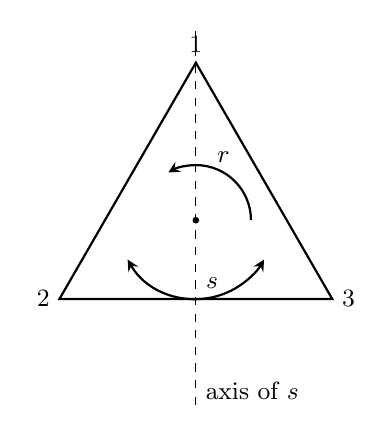
\begin{tikzpicture}[scale=2, every node/.style={font=\small}]
      % triangle vertices
      \coordinate (A) at (90:1);   % vertex 1 (top)
      \coordinate (B) at (210:1);  % vertex 2 (left)
      \coordinate (C) at (330:1);  % vertex 3 (right)
      % draw triangle
      \draw[thick] (A) -- (B) -- (C) -- cycle;
      % labels
      \node[above] at (A) {1};
      \node[left]  at (B) {2};
      \node[right] at (C) {3};

      % center
      \coordinate (O) at (0,0);
      \fill (O) circle (0.6pt);

      % dashed vertical axis (mirror axis for s)
      \draw[dashed] (0,1.2) -- (0,-1.2) node[above right] {axis of $s$};

      % small counter-clockwise rotation arrow for r
      \draw[->, >=stealth, thick] (0.35,0) arc (0:120:0.35) node[pos=0.5, above] {$r$};
      % double-headed curved arrow for s crossing the dashed axis (swap 2 <-> 3), small size
      \draw[<->, >=stealth, thick] (210:0.5) arc (210:330:0.5) node[pos=0.5, above right] {$s$};      
      \end{tikzpicture}
    \end{center}
  \end{define}



  
  \newpage
  \begin{enumerate}
    \item Find the order of every $a \in G$.
    \begin{subanswer}
      Let $G = S_3 = \{e, x, x^2, a, xa, x^2a\}$. The order of an element $g$, $o(g)$, is the smallest positive integer $m$ such that $g^m = e$.
      \begin{itemize}
        \item \textbf{Order 1:} $o(e) = 1$.
        \item \textbf{Order 2:} The elements of order 2 are the reflections.
        \begin{itemize}
          \item $o(a) = 2$, since $a^2 = e$.
          \item $o(xa) = 2$, since $(xa)^2 = (xa)(xa) = x(ax)a = x(x^2a)a = x^3a^2 = (e)(e) = e$.
          \item $o(x^2a) = 2$, since $(x^2a)^2 = (x^2a)(x^2a) = x^2(ax^2)a = x^2(xa)a = x^3a^2 = (e)(e) = e$.
        \end{itemize}
        \item \textbf{Order 3:} The elements of order 3 are the non-identity rotations.
        \begin{itemize}
          \item $o(x) = 3$, since $x^3 = e$.
          \item $o(x^2) = 3$, since $(x^2)^3 = x^6 = (x^3)^2 = e^2 = e$.
        \end{itemize}
      \end{itemize}
    \end{subanswer}

    \item Find all subgroups $H \subseteq G$. \textit{Hint: there are 6 for $S_3$}.
    \begin{subanswer}
      By Lagrange's Theorem, subgroups must have an order dividing $\abs{G}=6$. The possible orders are 1, 2, 3, and 6.
      \begin{itemize}
        \item \textbf{Order 1 (Trivial):} $H_1 = \{e\}$
        \item \textbf{Order 2 (Cyclic):} Generated by the three elements of order 2.
        \begin{itemize}
          \item $H_2 = \langle a \rangle = \{e, a\}$
          \item $H_3 = \langle xa \rangle = \{e, xa\}$
          \item $H_4 = \langle x^2a \rangle = \{e, x^2a\}$
        \end{itemize}
        \item \textbf{Order 3 (Cyclic):} Generated by the two elements of order 3.
        \begin{itemize}
          \item $H_5 = \langle x \rangle = \langle x^2 \rangle = \{e, x, x^2\}$
        \end{itemize}
        \item \textbf{Order 6 (The group itself):} $H_6 = G = \{e, x, x^2, a, xa, x^2a\}$
      \end{itemize}
    \end{subanswer}

    \item Identify $Z(G)$. Identify $\langle a \rangle$ and $C(a)$ for each $a \in G$.
    \begin{subanswer}
      \begin{itemize}
        \item \textbf{Center $Z(G)$:} The set of elements that commute with all 
        elements in $G$. Since $xa = ax^2 \neq ax$, $x$ does not commute with 
        $a$. Since the group is non-abelian, the center is a proper subgroup. 
        A quick check shows that only the identity commutes with all 6 elements.
          \[ Z(G) = \{e\} \]
        \item \textbf{Cyclic Subgroups $\langle a \rangle$:}
          \begin{itemize}
            \item $\langle e \rangle = \{e\}$
            \item $\langle x \rangle = \langle x^2 \rangle = \{e, x, x^2\}$
            \item $\langle a \rangle = \{e, a\}$
            \item $\langle xa \rangle = \{e, xa\}$
            \item $\langle x^2a \rangle = \{e, x^2a\}$
          \end{itemize}
        \item \textbf{Centralizers $C(a) = \{g \in G \mid ga = ag\}$:}
          \begin{itemize}
            \item $C(e) = G$
            \item $C(x) = \{g \mid gx = xg\}$. The elements that commute with $x$ are $e, x, x^2$.
              \[ C(x) = \{e, x, x^2\} \]
            \item $C(x^2) = \{g \mid gx^2 = x^2g\}$. Since $g$ commutes with $x^2$ iff it commutes with $x$,
              \[ C(x^2) = \{e, x, x^2\} \]
            \item $C(a) = \{g \mid ga = ag\}$. Only $e$ and $a$ commute with $a$.
              \[ C(a) = \{e, a\} \]
            \item $C(xa) = \{g \mid g(xa) = (xa)g\}$. Only $e$ and $xa$ commute with $xa$.
              \[ C(xa) = \{e, xa\} \]
            \item $C(x^2a) = \{g \mid g(x^2a) = (x^2a)g\}$. Only $e$ and $x^2a$ commute with $x^2a$.
              \[ C(x^2a) = \{e, x^2a\} \]
          \end{itemize}
      \end{itemize}
    \end{subanswer}

    \item For each subgroup $H$, find the equivalence classes under the relation $R_H$ in problem 6.
    \begin{subanswer}
      The relation is $(a, b) \in R_H$ if $ab^{-1} \in H$. The equivalence classes $[a] = \{b \mid ab^{-1} \in H\}$ are the \textbf{right cosets $Ha = \{ha \mid h \in H\}$}.
      \begin{itemize}
        \item \textbf{$H_1 = \{e\}$:} The cosets are the elements themselves.
          \begin{itemize}
            \item $[e] = \{e\}$, $[x] = \{x\}$, $[x^2] = \{x^2\}$, $[a] = \{a\}$, $[xa] = \{xa\}$, $[x^2a] = \{x^2a\}$
          \end{itemize}
        \item \textbf{$H_2 = \{e, a\}$:}
          \begin{itemize}
            \item $H_2e = \{e \cdot e, a \cdot e\} = \{e, a\}$
            \item $H_2x = \{e \cdot x, a \cdot x\} = \{x, ax\} = \{x, x^2a\}$
            \item $H_2x^2 = \{e \cdot x^2, a \cdot x^2\} = \{x^2, ax^2\} = \{x^2, xa\}$
          \end{itemize}
        \item \textbf{$H_3 = \{e, xa\}$:}
          \begin{itemize}
            \item $H_3e = \{e, xa\}$
            \item $H_3x = \{x, (xa)x\} = \{x, a\}$
            \item $H_3x^2 = \{x^2, (xa)x^2\} = \{x^2, x^2a\}$
          \end{itemize}
        \item \textbf{$H_4 = \{e, x^2a\}$:}
          \begin{itemize}
            \item $H_4e = \{e, x^2a\}$
            \item $H_4x = \{x, (x^2a)x\} = \{x, xa\}$
            \item $H_4x^2 = \{x^2, (x^2a)x^2\} = \{x^2, a\}$
          \end{itemize}
        \item \textbf{$H_5 = \{e, x, x^2\}$:} (This is a normal subgroup)
          \begin{itemize}
            \item $H_5e = \{e \cdot e, x \cdot e, x^2 \cdot e\} = \{e, x, x^2\}$
            \item $H_5a = \{e \cdot a, x \cdot a, x^2 \cdot a\} = \{a, xa, x^2a\}$
          \end{itemize}
        \item \textbf{$H_6 = G$:}
          \begin{itemize}
            \item $H_6e = G = \{e, x, x^2, a, xa, x^2a\}$
          \end{itemize}
      \end{itemize}
    \end{subanswer}

    \item For each $a \in G$, find its equivalence class under the relation $R$ from problem 7.
    \begin{subanswer}
      The relation is $(a, b) \in R$ if $b = g^{-1} a g$ for some $g \in G$. These are the \textbf{conjugacy classes}.
      \begin{itemize}
        \item \textbf{$[e]$:} The class of the identity is always just the identity.
          \[ [e] = \{g^{-1}eg \mid g \in G\} = \{e\} \]
        \item \textbf{$[x]$:} The class of rotations.
          \begin{itemize}
            \item $e^{-1}xe = x$
            \item $x^{-1}xx = x$
            \item $(x^2)^{-1}xx^2 = x(x)x^2 = x^4 = x$
            \item $a^{-1}xa = axa = a(ax^2) = x^2$
            \item $(xa)^{-1}x(xa) = (xa)x(xa) = (xa)(x^2a) = x(a x^2 a) = x(a(xa)) = x(x) = x^2$
            \item $(x^2a)^{-1}x(x^2a) = (x^2a)x(x^2a) = (xa)(x^2a) = x(ax^2a) = x(a(xa)) = x(x) = x^2$
          \end{itemize}
          \[ [x] = \{x, x^2\} \]
        \item \textbf{$[x^2]$:} Since $x^2 \in [x]$, $[x^2] = [x] = \{x, x^2\}$.
        \item \textbf{$[a]$:} The class of reflections.
          \begin{itemize}
            \item $e^{-1}ae = a$
            \item $x^{-1}ax = x^2(ax) = x^2(x^2a) = x^4a = xa$
            \item $(x^2)^{-1}ax^2 = x(ax^2) = x(xa) = x^2a$
          \end{itemize}
          (All other conjugates will also land in this set).
          \[ [a] = \{a, xa, x^2a\} \]
        \item \textbf{$[xa]$:} Since $xa \in [a]$, $[xa] = [a] = \{a, xa, x^2a\}$.
        \item \textbf{$[x^2a]$:} Since $x^2a \in [a]$, $[x^2a] = [a] = \{a, xa, x^2a\}$.
      \end{itemize}
      The distinct conjugacy classes are: $\{e\}$, $\{x, x^2\}$, and $\{a, xa, x^2a\}$.
    \end{subanswer}
  \end{enumerate}
  

  \newpage
  \item Repeat problem 8 where $G=D_8$, the dihedral group of order 8. 
  \textit{Hint: there are 10 subgroups}.
  \begin{enumerate}
    \item Find the order of every $a \in G$.
    \begin{subanswer}
      The elements of $D_8$ are: $e$, $r$, $r^2$, $r^3$, $s$, $sr$, $sr^2$, $sr^3$.
      \begin{itemize}
        \item $o(e) = 1$
        \item $o(r) = 4$
        \item $o(r^2) = 2$
        \item $o(r^3) = 4$
        \item $o(s) = 2$
        \item $o(sr) = 2$
        \item $o(sr^2) = 2$
        \item $o(sr^3) = 2$
      \end{itemize}
    \end{subanswer}
    \item Find all subgroups $H \subseteq G$. \textit{Hint: there are 6 for $S_3$}.
    \begin{subanswer}
      The subgroups of $D_8$ are:
      \begin{itemize}
        \item $H_1 = \{e\}$
        \item $H_2 = \{e, r^2\}$
        \item $H_3 = \{e, r, r^2, r^3\}$
        \item $H_4 = \{e, s\}$
        \item $H_5 = \{e, sr^2\}$
        \item $H_6 = D_8$
      \end{itemize}
    \end{subanswer}
    \item Identify $Z(G)$. Identify $(a)$ and $C(a)$ for each $a \in G$.
    \begin{subanswer}
      The center $Z(G)$ consists of all elements that commute with every element of $G$. In $D_8$, we have:
      \begin{itemize}
        \item $Z(D_8) = \{e, r^2\}$
      \end{itemize}
      The centralizer $C(a)$ for each $a \in G$ is:
      \begin{itemize}
        \item $C(e) = D_8$
        \item $C(r) = \{e, r, r^2, r^3\}$
        \item $C(r^2) = D_8$
        \item $C(r^3) = \{e, r, r^2, r^3\}$
        \item $C(s) = \{e, s\}$
        \item $C(sr) = \{e, sr\}$
        \item $C(sr^2) = \{e, sr^2\}$
        \item $C(sr^3) = \{e, sr^3\}$
      \end{itemize}
    \end{subanswer}
    \item For each subgroup $H$, find the equivalence classes under the relation $R_H$ in problem 6.
    \begin{subanswer}
      The equivalence classes under the relation $R_H$ are:
      \begin{itemize}
        \item For $H_1 = \{e\}$: Each element forms its own class.
        \item For $H_2 = \{e, r^2\}$: Classes are $\{e, r^2\}$, $\{r, r^3\}$, $\{s, sr^2\}$, $\{sr, sr^3\}$.
        \item For $H_3 = \{e, r, r^2, r^3\}$: Classes are $\{e, r, r^2, r^3\}$ and $\{s, sr, sr^2, sr^3\}$.
        \item For $H_4 = \{e, s\}$: Classes are $\{e, s\}$, $\{r, sr\}$, $\{r^2, sr^2\}$, $\{r^3, sr^3\}$.
        \item For $H_5 = \{e, sr^2\}$: Classes are $\{e, sr^2\}$, $\{r, sr^3\}$, $\{r^2, s\}$, $\{r^3, sr\}$.
        \item For $H_6 = D_8$: The entire group is one class.
      \end{itemize}
    \end{subanswer}
    \item For each $a \in G$, find its equivalence class under the relation $R$ from problem 7.
    \begin{subanswer}
      The conjugacy classes in $D_8$ are:
      \begin{itemize}
        \item $[e] = \{e\}$
        \item $[r] = \{r, r^3\}$
        \item $[r^2] = \{r^2\}$
        \item $[s] = \{s, sr^2\}$
        \item $[sr] = \{sr, sr^3\}$
      \end{itemize}
      The conjugacy classes partition the group $D_8$ into disjoint subsets.
    \end{subanswer}
  \end{enumerate}

  \newpage
  \item Repeat problem 8 where $G=\left(\setZ_n,+\right)$ for 
  $n=3,4,5,6$ and for $V_4$ from problem 1.
  \begin{enumerate}
    \item Find the order of every $a \in G$.
    \begin{subanswer}
      The elements of $\setZ_n$ are $\{[0], [1], [2], \ldots, [n-1]\}$. 
      The order of each element is:
      \begin{itemize}
        \item For $n=3$: $o([0])=1$, $o([1])=3$, $o([2])=3$.
        \item For $n=4$: $o([0])=1$, $o([1])=4$, $o([2])=2$, $o([3])=4$.
        \item For $n=5$: $o([0])=1$, $o([1])=5$, $o([2])=5$, $o([3])=5$, $o([4])=5$.
        \item For $n=6$: $o([0])=1$, $o([1])=6$, $o([2])=3$, $o([3])=2$, $o([4])=3$, $o([5])=6$.
      \end{itemize}
      The orders of the elements in $\setZ_n$ are determined by the divisors of $n$.
    \end{subanswer}
    \item Find all subgroups $H \subseteq G$. \textit{Hint: there are 6 for $S_3$}.
    \begin{subanswer}
      The subgroups of $\setZ_n$ are:
      \begin{itemize}
        \item For $n=3$: $\{[0]\}$, $\{[0], [1], [2]\}$.
        \item For $n=4$: $\{[0]\}$, $\{[0], [2]\}$, $\{[0], [1], [2], [3]\}$.
        \item For $n=5$: $\{[0]\}$, $\{[0], [1], [2], [3], [4]\}$.
        \item For $n=6$: $\{[0]\}$, $\{[0], [2], [4]\}$, $\{[0], [1], [2], [3], [4], [5]\}$.
      \end{itemize}
      The subgroup structure is determined by the divisors of $n$.
    \end{subanswer}
    \item Identify $Z(G)$. Identify $(a)$ and $C(a)$ for each $a \in G$.
    \begin{subanswer}
      Since $\setZ_n$ is abelian, $Z(G) = G$ for all $n$.
      The cyclic subgroup generated by each element $[a]$ is 
      $\langle [a] \rangle = \{[ka] \mid k \in \setZ\}$.
      The centralizer $C([a]) = G$ for all $[a]$ since the group is abelian.
    \end{subanswer}
    \item For each subgroup $H$, find the equivalence classes under the relation $R_H$ in problem 6.
    \begin{subanswer}
      The equivalence classes under the relation $R_H$ are the cosets of $H$ in $G$.
      Since $\setZ_n$ is abelian, the left and right cosets coincide.
      For each subgroup $H$, the cosets partition $G$ into disjoint subsets.
      The equivalence classes are:
      \begin{itemize}
        \item For $n=3$: $\{[0]\}$, $\{[1], [2]\}$.
        \item For $n=4$: $\{[0]\}$, $\{[2]\}$, $\{[1], [3]\}$.
        \item For $n=5$: $\{[0]\}$, $\{[1], [2], [3], [4]\}$.
        \item For $n=6$: $\{[0]\}$, $\{[2], [4]\}$, $\{[1], [3], [5]\}$.
      \end{itemize}
    \end{subanswer}
    \item For each $a \in G$, find its equivalence class under the relation $R$ from problem 7.
    \begin{subanswer}
      Since $\setZ_n$ is abelian, each element forms its own conjugacy class.
      Thus, for each $[a] \in \setZ_n$, the equivalence class is:
      \[
        [ [a] ] = \{ [a] \}
      \]
      for all $n=3,4,5,6$.
    \end{subanswer}
  \end{enumerate}
\end{enumerate}

































































\newpage\handout[true]
{\textsc{Math 2106-B: Foundations of Mathematical Proof}}{Fall 2025}
{Homework 7: More on Groups and Isomorphisms}
{\textit{Prof.} \href{https://ceheitsch.github.io/webpage/}{Dr. Christine Heitsch}}{Due Date: October 30, 2025}
{Math 2106-B: HW7}
{\large
  \noindent
  \textbf{Name:} \HandoutAuthor \smallskip \\

  \noindent
  \textbf{GTID:} 903743506 \smallskip \\

  \noindent
  %%% List anyone with whom you discussed the problems
  \textbf{Collaborators:} None. This material reflects independent preparation. \smallskip \\

  \noindent
  %%% List all resources used OTHER than the textbook, lecture notes, 
  %%% webwork problems, ICA questions, and previous homework assignments.
  \textbf{Outside resources:} This work was informed by MATH 2106 course materials 
  (ICAs: in-class activities and WebWork contents) from \HandoutInstitution\ (the course textbook is 
  Chartrand \parencite{chartrand_mathematical_2018}).   
  Outside references specifically include
  textbooks written by 
  Grimaldi \parencite{grimaldi_discrete_2004} (used in MATH 3012) and 
  Rosen \parencite{rosen_discrete_2019} (used in CS 2050). \smallskip \\

  \noindent
  \textbf{Notice}: The answers contain cross-references throughout this document as clickable hyperlinks in most PDF viewers. However, the Gradescope PDF view might not support clickable hyperlinks.
}
\printbibliography[
  heading=bibintoc,   
  title={References}     % change “References” text if needed
]
% `heading=bibnumbered` if you prefer it numbered chapter (in \tableofcontents)
% `heading=bibintoc`    if you prefer it unnumbered but still in the ToC
\newpage
% \printbibliography[
  heading=bibintoc,   
  title={References}     % change “References” text if needed
]
% `heading=bibnumbered` if you prefer it numbered chapter (in \tableofcontents)
% `heading=bibintoc`    if you prefer it unnumbered but still in the ToC\newpage
% The following table presents the standard logical equivalences from these sources together with 
the author's own (or the student, myself, Jaehoon Song) clarifications and labels where applicable.


\begin{table}[h!]
  \centering
  \renewcommand{\arraystretch}{1.2}
  \setlength{\tabcolsep}{8pt}
  \begin{tabular}{|p{5.0cm}|p{5.0cm}|p{5.2cm}|}
    \hline
    \rowcolor[HTML]{E0E0E0}
    \multicolumn{2}{|l|}{\textbf{Logical Equivalences}} & \textbf{Name} \\
    \hline
    $\,p \AND q \equiv q \AND p$ & $\,p \OR q \equiv q \OR p$ & Commutative Law \\
    \hline
    $\, (p \AND q) \AND r \equiv p \AND (q \AND r)$ & $\, (p \OR q) \OR r \equiv p \OR (q \OR r)$ & Associative Law \\
    \hline
    $\,p \AND (q \OR r) \equiv (p \AND q) \OR (p \AND r)$ & $\,p \OR (q \AND r) \equiv (p \OR q) \AND (p \OR r)$ & Distributive Law \\
    \hline
    $\,\overline{p \AND q} \equiv \sNOT{p} \OR \sNOT{q}$ & $\,\overline{p \OR q} \equiv \sNOT{p} \AND \sNOT{q}$ & DeMorgan's Law \\
    \hline
    \multicolumn{2}{|l|}{$\,\overline{\overline{p}} \equiv p$} & Double Negation law \\
    \hline
    $\,p \AND \boldsymbol{T} \equiv p$ & $\,p \OR \boldsymbol{F} \equiv p$ & Identity Law \\
    \hline
    $\,p \OR \boldsymbol{T} \equiv \boldsymbol{T}$ & $\,p \AND \boldsymbol{F} \equiv \boldsymbol{F}$ & Domination Law \\
    \hline
    $\,p \AND p \equiv p$ & $\,p \OR p \equiv p$ & Idempotent Law \\
    \hline
    \multicolumn{2}{|l|}{$\,p \THEN q \equiv \sNOT{p} \OR q$} & Implication Equivalence \\
    \hline
    \multicolumn{2}{|l|}{$\,\overline{p \THEN q} \equiv p \AND \sNOT{q}$} & Negation of Implication \\
    \hline
    \multicolumn{2}{|l|}{$\,p \THEN q \equiv \sNOT{q} \THEN \sNOT{p}$} & Contrapositive Equivalence \\
    \hline
    \multicolumn{2}{|l|}{$\,p \OR \sNOT{p} \equiv \boldsymbol{T}$} & Law of Tautology \\
    \hline
    \multicolumn{2}{|l|}{$\,p \AND \sNOT{p} \equiv \boldsymbol{F}$} & Law of Contradiction \\
    \hline
  \end{tabular}
\end{table}\newpage
% 
The following definitions are presented from standard mathematical sources (\textbf{Sets}).
Clarifications and labels have been added where applicable.

\begin{define}{Basic Set Concepts}\phantomsection\label{def:basic-set-concepts} % \hyperref[def:basic-set-concepts]{YOUR_CONTEXT}
  \begin{enumerate}
    \item \textbf{Universal Set:} A universal set $\setUNIV$ is a
    set that contains all objects under consideration in a particular context or problem.
    \item \textbf{Empty Set:} The empty set, denoted $\setNULL$,
    is the unique set that contains no elements.
    \item \textbf{Subset:} Let $A$ and $B$ be sets. $A$ is a
    subset of $B$ ($A \subseteq B$) if (and only if)
    for all $x \in A$, $x \in B$.
    \item \textbf{Set Equality:} Let $A$ and $B$ be sets. The sets $A$ and $B$ are
    equal ($A = B$) if $A \subseteq B$ and $B \subseteq A$.
    \item \textbf{Power Set:} Let $A$ be a set. The power set of $A$, denoted $\sPOWER{A}$ or $2^A$,
    is the set of all subsets of $A$. That is, $\mathcal{P}(A) = \{S\in\setUNIV : S \subseteq A\}$.
  \end{enumerate}
\end{define}
The following definitions extend the understanding of set operations
and properties.


\begin{define}{Set Operations}\phantomsection\label{def:set-operations} % \hyperref[def:set-operations]{YOUR_CONTEXT}
  \begin{enumerate}
    \item \textbf{Complementary Set:} Let $A$ be a subset of the universal set $\setUNIV$.
    The complement of $A$, denoted $A^c$ or $\overline{A}$, is the set of all elements
    in $\setUNIV$ that are not in $A$. That is, $A^c = \{x \in \setUNIV : x \notin A\}$.
    \item \textbf{Union:} Let $A$ and $B$ be sets. The union of $A$ and $B$,
    denoted $A \cup B$, is the set of all elements that are in $A$, or in $B$, or in both.
    That is, $A \cup B = \{x : x \in A \lor x \in B\}$.
    \item \textbf{Intersection:} Let $A$ and $B$ be sets. The intersection of $A$ and $B$,
    denoted $A \cap B$, is the set of all elements that are in both $A$ and $B$.
    That is, $A \cap B = \{x : x \in A \land x \in B\}$.
    \item \textbf{Set Difference:} Let $A$, $B$ be subsets of a universal set $\setUNIV$.
    The set difference $A \sMINUS B$ is defined to be the set
    $\{ x \in \setUNIV \LDIV x \in A \text{ and } x \notin B\}$. \vspace*{10px}\\
    \textit{It is sometimes called the relative complement of $B$ in $A$,
    and denoted in the textbook as $A - B$.}
    \item \textbf{Cartesian Product:} Let $A$ and $B$ be sets. The Cartesian product of
    $A$ and $B$, denoted $A \sTIMES B$, is the set consisting of all ordered pairs:
    \[
    A \sTIMES B = \{(a, b) \LDIV a \in A, b \in B\}.
    \]
  \end{enumerate}
\end{define}


\newpage

The following claims are given in the reference as well. Let $A,B\in U$, a universal set.


\begin{claim}{Subset of Union: $A \subseteq \sOR{A}{B}$}\phantomsection\label{claim:subset-union} % \hyperref[claim:subset-union]{YOUR_CONTEXT}
  \begin{subprove}[bluecolor]
      Let $x\in U$, assume $x\in A$. Then the statement \inlinequote{$x\in A$ or $x\in B$} is true.
      Hence, by the definition, $\sOR{A}{B}=\{x\in U\LDIV x\in A$ or $x\in B\}$, $x\in \sOR{A}{B}$.
      Thus, $A \subseteq \sOR{A}{B}$.
  \end{subprove}
\end{claim}

\begin{claim}{Empty Subset: $\setNULL \subseteq A$}\phantomsection\label{claim:empty-subset} % \hyperref[claim:empty-subset]{YOUR_CONTEXT}
  \begin{subprove}[bluecolor]
      Let $x\in U$, assume $x\in \setNULL$. But there are no elements in $\setNULL$, so
      $x\in \setNULL$ is false. Since the premise is false, the implication if $x\in \setNULL$,
      then $x\in A$ is true. Thus, $\setNULL \subseteq A$ by definition of \hyperref[def:basic-set-concepts]{subsets}.
  \end{subprove}
\end{claim}

\begin{claim}{Subset as Equality: $\sOR{A}{B}=A$ if and only if $B\subseteq A$}\phantomsection\label{claim:subset-equality} % \hyperref[claim:subset-equality]{YOUR_CONTEXT}
  \begin{subprove}[bluecolor]
      Let $x\in U$, first, we assume $B\subseteq A$, we have already shown
      $A \subseteq \sOR{A}{B}$ by the claim, \hyperref[claim:subset-union]{Subset of Union}. 
      To show $\sOR{A}{B} \subseteq A$, assume $x\in \sOR{A}{B}$.
      By definition, $x\in A$ or $x\in B$. Considering $x\in B$ and assumption
      $B \subseteq A$, $x\in B$ implies $x\in A$. Thus, $\sOR{A}{B} \subseteq A$.
      Hence, if $B\subseteq A$, then $\sOR{A}{B} = A$. \vspace*{10px}\\
      Now, we assume $\sOR{A}{B}=A$. To show $B\subseteq A$, we now assume $x\in B$. Since $x\in B$, by definition
      of union, $x\in \sOR{A}{B} = A$. Therefore, $B\subseteq A$.
  \end{subprove}
\end{claim}


%%%%%%%%%%%%%%%%%%% 9/8/25

Let $\setUNIV$ be a set. 
\begin{claim}{ICA6}\phantomsection\label{claim:ica6} % \hyperref[claim:ica6]{YOUR_CONTEXT}
  For all $A,B\in\setUNIV$, $$A\sTIMES B =\setNULL\THEN \group{A=\setNULL\OR B=\setNULL}$$
  \begin{subprove}[bluecolor]
    Let $A,B\in\setUNIV$. We prove $A\sTIMES B=\setNULL$. Assume it is not the case that 
    $A=\setNULL$ or $B=\setNULL$. Thus, we have $A=\setNULL$ and $B=\setNULL$. 
    Since $A\ne\setNULL$ by assumption, there exists an element $a\in A$. Likewise, there 
    is some $b\in B$ since $B\ne\setNULL$. Thus, $\group{a,b}\in\sBUILD{(x,y)}{x\in A,y\in B}$ 
    by definition. But then, $A\sTIMES B\ne\setNULL$ by definition. Hence, the claim holds. 
  \end{subprove}
\end{claim}


\begin{define}{Relatively Prime Integers (Coprime)}\phantomsection\label{def:relatively-prime} % \hyperref[def:relatively-prime]{YOUR_CONTEXT}
  Let $x,y \in \mathbb{Z}$. The integers $x$ and $y$ are said to be
  \textbf{relatively prime} if and only if
  $\gcd(x,y) = 1$.
\end{define}
\newpage
% The following definitions and axioms are presented from standard mathematical sources (\textbf{Number Theory}) together with the author's own (or the student, myself, Jaehoon Song) clarifications and labels where applicable.

\begin{define}{Integers}[def:integers][red]
  $\setZ$: the set of all integers
\end{define}

\begin{define}{Rational Numbers}[def:rational-numbers][red]
  $\setQ$: the set of all rational numbers
\end{define}

\begin{define}{Real Numbers}[def:real-numbers][red]
  $\setR$: the set of all real numbers
\end{define}

\begin{define}{Natural Numbers}[def:natural-numbers][red]
  $\setN$ or $\setZ_{>0}$: the set of all natural numbers which are the set of positive integers (not including $0$)
\end{define}

\begin{define}{Positive Real Numbers}[def:positive-real-numbers][red]
  $\setR_{>0}$: the set of all positive real numbers
\end{define}

\begin{define}{Non-negative Real Numbers}[def:non-negative-real-numbers][red]
  $\setR_{\geq 0}$: the set of all non-negative real numbers
\end{define}


\newpage

The following definitions and claims extend the understanding of integers.

Here are the ICA2 Definitions and Axioms as follows.

\begin{define}{Even Integer}[def:even-integer][red]
  An integer $n$ is \underbar{even} if there exists 
  (existential quantification logic $\exists$) an integer $k$ such that
  \[
  n = 2k.
  \]
\end{define}

\begin{define}{Odd Integer}[def:odd-integer][red]
  An integer $n$ is \underbar{odd} if 
  there exists some integer $k$ such that
  \[
  n = 2k + 1.
  \]
\end{define}

\begin{define}{Closure under Addition}[def:closure-addition][red]
  The sum of two integers is again an 
  integer. (Closure under addition)
\end{define}

\begin{define}{Closure under Multiplication}[def:closure-multiplication][red]
  The product of two integers is again 
  an integer. (Closure under multiplication)
\end{define}

\begin{define}{Odd if and only if Not Even}[def:odd-iff-not-even][red]
  An integer is odd if and only if it 
  is not even.
\end{define}

Here are the ICA3 Definitions and Axioms as follows.

\begin{define}{Universal Closure under Addition}[def:universal-closure-addition][red]
  The sum of two integers (Universal quantification for all, for every, for each) is again an integer. (Closure under addition)
\end{define}

\begin{define}{Universal Closure under Multiplication}[def:universal-closure-multiplication][red]
  The product of two integers (Universal quantification for all, for every, for each) is again an integer. (Closure under multiplication)
\end{define}

\begin{define}{Even Integer Square}[def:even-integer-square][red]
  An integer $n$ is even if and only if $n^2$ is even.
\end{define}

\newpage

The following claims are given in the reference as well.

\begin{define}{Sum of Even Integers}[claim:sum-even-integers][red]
  The sum of two even integers is again an even integer.
  \begin{subprove}[red]
    Let $x$ be an integer and $y$ be an integer ($\forall x,y \in \setZ$). 
    Suppose $x$ is even and $y$ is even. Then, by \nameref{def:even-integer}, there exists an integer 
    $k$ and an integer $j$ such that $x=2k$ and $y=2j$. Then, 
    $x+y=\left(2k\right)+\left(2j\right)=2\left(k+j\right)$. By \nameref{def:closure-addition}, since $k$ and 
    $j$ are integers, then so is $\left(k+j\right)$. Hence, by definition, $x+y$ is an 
    even integer.
  \end{subprove}
\end{define}

The following definitions extend the understanding of integers including divisibility.

\begin{define}{Divisibility}[def:divisibility][red]
  An integer $n$ divides an integer $m$, denoted $n \LDIV m$, if there 
  exists an integer $k$ such that $m=n k$. Otherwise, $n \nmid m$.
\end{define}

The following definitions extend the classification of real numbers into rational and irrational numbers.

\begin{define}{Rational Number}[def:rational-number][red]
  A real number $x$ is \underbar{rational} if there exist integers $a$ and $b$ with $b \neq 0$ such that $bx = a$.
  Otherwise, $x$ is \underbar{irrational}.

  \textbf{Note}: Compare the rational number definition with the even/odd axiom \inlinequote{odd iff not even} from \nameref{def:odd-iff-not-even}.
\end{define}

The following claims are given in the reference as well.

\begin{define}{Irrationality of $\sqrt{2}$}[claim:sqrt2-irrational][red]
  $\sqrt{2}$ is irrational.
  \begin{subprove}[red]
    Suppose $\sqrt{2}$ is rational. Then, by \nameref{def:rational-number}, there exists $a,b\in \setZ$ 
    with $b\ne 0$ such that $b\cdot\sqrt{2}=a$. We may further assume that any factors 
    common to $a$ and $b$ have already been removed.\\

    Then, squaring both sides, this yields $2\cdot b^2 = a^2$.
    Since products of integers are again integers by \nameref{def:closure-multiplication}, we have that $a^2,b^2\in \setZ$.
    Thus, by definition, $a^2$ is even. Therefore, by \nameref{def:even-integer-square}, $a$ is even. 
    Thus, there exists $c\in\setZ$ such that $a=2c$. Then
    $$
    2b^2=a^2={2c}^2=4c^2
    $$
    Then, $b^2=2c^2$. Then, as before, $b^2$ is even, so $b$ is even.
    However, $a$ and $b$ both being even contradicts the fact that any factors 
    common to $a$ and $b$ have already been removed.
  \end{subprove}
\end{define}






%%%%%%%%%%%%%%%%%%% New style (refactor model)
\begin{define}{Relatively Prime Integers (Coprime)}[def:relatively-prime][red]
  Let $x,y \in \mathbb{Z}$. The integers $x$ and $y$ are said to be
  \textbf{relatively prime} if and only if
  $\gcd(x,y) = 1$.
\end{define}\newpage
%%%%%%%%%%%%%%%%%%%%%%%%%%%%%%%%%%%%%%%%%%%%%%%%%%%%%%%%%%%%%%%%%%%%%%%
% References Section
%%%%%%%%%%%%%%%%%%%%%%%%%%%%%%%%%%%%%%%%%%%%%%%%%%%%%%%%%%%%%%%%%%%%%%%
\textbf{Remark}: The following definitions (or results) are already proved in class or on previous ICA, 
Wbwk, Hmwk assignments, and contents of the textbook.
\begin{define}{Groups}[def:group][red]
  A \textbf{group} is a nonempty set \(G\) under the (binary) 
  operation \(*: S \times S \to S\), denoted by \((G, *)\), such that
  \begin{itemize}
    \item \textbf{Closure:} For all \(a, b \in G\), \(a * b \in G\).
    \item \textbf{Associativity:} For all \(a, b, c \in G\), \((a * b) * c = a * (b * c)\).
    \item \textbf{Existence of Identity:} There exists an element \(e \in G\) 
    such that for all \(a \in G\), \(e * a = a * e = a\).
    \item \textbf{Existence of Inverse:} For each \(a \in G\), there exists an 
    element \(a^{-1} \in G\) such that \(a * a^{-1} = a^{-1} * a = e\).
  \end{itemize}
\end{define}
Let $(G, *)$ be a group with identity $e \in G$.
\begin{define}{Subgroup}[def:subgroup][red]
  A nonempty subset $H$ of $G$ is called a subgroup of $G$ if (and only if) $(H, *)$is a group. (That is, $H$ itself is a group with respect to the product of $G$.)
\end{define}
\begin{define}{Subgroup Lemma}[lem:subgroup-lemma][red]
  (To be proved on ICA15.) A subset $H \subseteq G$ is a subgroup of $(G, *)$if (and only if) 
  $H$ is nonempty, closed under the product of $G$, and contains inverses, i.e 
  \begin{enumerate}
    \item $H \neq \emptyset$,
    \item for all $a, b \in H$, $a * b \in H$, and
    \item for all $a \in H, a^{-1} \in H$.
  \end{enumerate}
\end{define}
\begin{define}{Exponent Notation}[def:exponent-notation][red]
  For $a \in G$, define $a^0=e$. 
  For $i \in \setZ$ with $i \geq 1$, 
  define $a^i=a * a^{i-1}$ and $a^{-i}=\left(a^{-1}\right)^i$. 
  It follows that $a^n a^m=a^{n+m}$ and $\left(a^n\right)^m=a^{n m}$ for $n, m \in \setZ$.
\end{define}
\begin{define}{Order of an Element}[def:order-of-an-element][red]
  Let $G$ be a finite group. The \textbf{order} of an 
  element $a \in G$, denoted $o(a)$, is the least positive 
  integer $m$ such that $a^m=e$.
\end{define}
\begin{define}{Abelian Group}[def:abelian-group][red]
  A group $(G, *)$ is called an \textbf{abelian group} (or \textbf{commutative group}) if for all $a, b \in G$, 
  \[
    a * b = b * a.
  \]
\end{define}
\begin{define}{Cyclic Subgroup}[def:cyclic-subgroup][red]
  The cyclic subgroup generated by $a \in G$ is the 
  set, $\left(a\right)=\left\{a^i \mid i \in \setZ\right\}$.
\end{define}
\begin{define}{Symmetric Group}[def:symmetric-group][red]
  The symmetric group of degree $n$, denoted $S_n$, is the group of all permutations (bijective maps) of the set $\{1,\dots,n\}$ with composition as the group operation:
  \[
    S_n=\{\sigma:\{1,\dots,n\}\to\{1,\dots,n\}\mid \sigma\ \text{is a bijection}\}
  \]
  Note that $\abs{S_n}=n!$.
\end{define}


%%%%%%%%%%%%%%%%%%%%%%%%%%%%%%%%%%%%%%%%%%%%%%%%%%%%%%%%%%%%%%%%%%%%%%%
% Problems Section
%%%%%%%%%%%%%%%%%%%%%%%%%%%%%%%%%%%%%%%%%%%%%%%%%%%%%%%%%%%%%%%%%%%%%%%
\newpage
Let $G$ be a group with identity $e$.
\begin{enumerate}
  \item Prove or disprove from the definitions:
  \begin{enumerate}
    \item A cyclic group is abelian.
    \begin{define}{Cyclic Group}[def:cyclic-group][red]
      A group $(G, *)$ is called a \textbf{cyclic group} if there exists an element $g \in G$ such that $G = (g) = \{g^i \mid i \in \setZ\}$, 
      where $(g)$ is the cyclic subgroup generated by $g$ as defined in \nameref{def:cyclic-subgroup}. 
      The element $g$ is called a \textbf{generator} of $G$.
    \end{define}
    \begin{subprove}
      Let $(G, *)$ be a cyclic group and let $g \in G$ be a generator of $G$ such that $G = (g) = \{g^i \mid i \in \setZ\}$.
      Let $a, b \in G$ be arbitrary elements.
      Since $G$ is cyclic, there exist integers $m, n \in \setZ$ such that $a = g^m$ and $b = g^n$.
      By the \nameref{def:exponent-notation},
      \[
        a * b = g^m * g^n = g^{m+n} = g^{n+m} = g^n * g^m = b * a.
      \]
      Since $a$ and $b$ were arbitrary elements of $G$, it follows that for all $a, b \in G$, $a * b = b * a$.
      Therefore, by definition of \nameref{def:abelian-group}, $G$ is an abelian group.
    \end{subprove}
    \item An abelian group is cyclic.
    \begin{subdisprove}
      Let $V_4 = \setZ_2 \times \setZ_2$ be the Klein 4-group under coordinate-wise addition, 
      which was shown to be an abelian group in Homework 6.
      The elements of $V_4$ are $\{([0],[0]), ([0],[1]), ([1],[0]), ([1],[1])\}$.
      
      For $V_4$ to be cyclic, there must exist an element $g \in V_4$ such that $(g) = V_4$.
      However, it is observed that:
      \begin{itemize}
        \item The element $([0],[0])$ is the identity and generates only itself.
        \item The element $([0],[1])$ satisfies $([0],[1])^2 = ([0],[0])$, so $( ([0],[1]) ) = \{([0],[0]), ([0],[1])\}$.
        \item The element $([1],[0])$ satisfies $([1],[0])^2 = ([0],[0])$, so $( ([1],[0]) ) = \{([0],[0]), ([1],[0])\}$.
        \item The element $([1],[1])$ satisfies $([1],[1])^2 = ([0],[0])$, so $( ([1],[1]) ) = \{([0],[0]), ([1],[1])\}$.
      \end{itemize}
      Since no element generates all four elements of $V_4$, it is concluded that $V_4$ is not cyclic.
      Thus, $V_4$ is an abelian group that is not cyclic.
      
      Therefore, by counterexample, the statement that an abelian group is cyclic is false.
    \end{subdisprove}
  \end{enumerate}




  \newpage
  \item If $G$ is cyclic, prove that every subgroup of $G$ is cyclic.
  \begin{define}{Well-Ordering Principle}[def:well-ordering][red]
    Every nonempty subset of the positive integers $\setZ^+$ has a least element. 
    That is, if $S \subseteq \setZ^+$ and $S \neq \emptyset$, then there exists $m \in S$ such that $m \leq n$ for all $n \in S$.
  \end{define}
  \begin{define}{Division Algorithm}[def:division-algorithm][red]
    For any integers $n$ and $d \neq 0$, there exist unique integers $q$ (quotient) and $r$ (remainder) such that 
    $n = qd + r$ and $0 \leq r < |d|$. If $d > 0$, then $0 \leq r < d$.
  \end{define}
  \begin{subprove}
    Let $(G, *)$ be a cyclic group with generator $g \in G$ such that $G = (g) = \{g^i \mid i \in \setZ\}$.
    Let $H$ be a subgroup of $G$ for the sake of direct proof.
    
    Two cases are considered.
    
    \textbf{Case 1:} If $H = \{e\}$, where $e$ is the identity element of $G$, then $H$ is cyclic since it is generated by $e$.
    
    \textbf{Case 2:} If $H \neq \{e\}$, then $H$ contains at least one non-identity element.
    Since $H \subseteq G = (g)$ and $H \neq \{e\}$, there exists an integer $k \neq 0$ such that $g^k \in H$.
    
    By the \nameref{def:well-ordering}, let $d$ be the smallest positive integer such that $g^d \in H$.
    It is claimed that $H = (g^d)$.
    
    To show that $H \subseteq (g^d)$, let $h \in H$ be arbitrary.
    Since $h \in H \subseteq G = (g)$, there exists an integer $n \in \setZ$ such that $h = g^n$.
    By the \nameref{def:division-algorithm}, there exist integers $q$ and $r$ with $0 \leq r < d$ such that $n = qd + r$.
    It follows that
    \[
      h = g^n = g^{qd + r} = (g^d)^q * g^r.
    \]
    Since $g^d \in H$ and $H$ is a subgroup, $(g^d)^q \in H$ by closure under the group operation.
    Moreover, since $h \in H$ and $(g^d)^q \in H$, it follows that $g^r = h * ((g^d)^q)^{-1} \in H$ by closure and existence of inverses in $H$.
    
    However, since $d$ is the smallest positive integer such that $g^d \in H$ and $0 \leq r < d$, 
    the only possibility is that $r = 0$.
    Therefore, $h = (g^d)^q \in (g^d)$.
    Since $h$ was arbitrary, it is concluded that $H \subseteq (g^d)$.
    
    To show that $(g^d) \subseteq H$, since $g^d \in H$ and $H$ is a subgroup, 
    it follows by closure under the group operation that $(g^d) = \{(g^d)^i \mid i \in \setZ\} \subseteq H$.
    
    Therefore, $H = (g^d)$, and hence $H$ is cyclic by definition of \nameref{def:cyclic-group}.
    
    In both cases, it is shown that $H$ is cyclic.
    Since $H$ was an arbitrary subgroup of $G$, it follows that every subgroup of $G$ is cyclic.
  \end{subprove}





  \newpage
  
  \item A subgroup is \textit{proper} if it is neither the identity 
  nor the entire group. Prove that if $G$ has no proper subgroups, 
  then $G$ is cyclic. \textit{Do not assume that $G$ is finite}.
  \begin{define}{Proper Subgroup}[def:proper-subgroup][red]
    A subgroup $H$ of $G$ is called a \textbf{proper subgroup} if $H \neq \{e\}$ and $H \neq G$, 
    where $e$ is the identity element of $G$.
  \end{define}
  \begin{subprove}
    Let $(G, *)$ be a group with identity $e$ and suppose that $G$ has no proper subgroups for the sake of direct proof.
    
    Two cases are considered.
    
    \textbf{Case 1:} If $G = \{e\}$, then $G$ is cyclic since it is generated by $e$.
    
    \textbf{Case 2:} If $G \neq \{e\}$, then $G$ contains at least one non-identity element.
    Let $g \in G$ be an arbitrary non-identity element, i.e., $g \neq e$.
    
    Consider the cyclic subgroup $(g) = \{g^i \mid i \in \setZ\}$ generated by $g$, 
    as defined in \nameref{def:cyclic-subgroup}.
    By definition of \nameref{def:subgroup}, $(g)$ is a subgroup of $G$.
    
    Since $g \neq e$, it follows that $(g) \neq \{e\}$.
    Moreover, since $G$ has no proper subgroups, $(g)$ cannot be a proper subgroup of $G$.
    Therefore, it must be that $(g) = G$.
    
    Since $G = (g)$ and $g \in G$, it is concluded by definition of \nameref{def:cyclic-group} that $G$ is cyclic, 
    with $g$ as a generator.
    
    In both cases, it is shown that $G$ is cyclic.
    Since $g$ was an arbitrary non-identity element of $G$ in Case 2, 
    it follows that every non-identity element of $G$ generates $G$.
  \end{subprove}







  
  \item Let $H$ be a nonempty subset of $G$ such that $a b^{-1} \in H$ for all $a, b \in H$. Prove that $H$ is a subgroup of $G$.
  \begin{subprove}
    Let $H$ be a nonempty subset of $G$ such that $a b^{-1} \in H$ for all $a, b \in H$ for the sake of direct proof.
    It is shown that $H$ satisfies the conditions of \nameref{lem:subgroup-lemma}.
    
    \begin{itemize}
      \item \textbf{Nonemptyness:} By hypothesis, $H$ is nonempty.
      
      \item \textbf{Existence of Identity:} Since $H$ is nonempty, there exists an element $a \in H$.
      Taking $a = b$ in the given condition, it follows that $a a^{-1} = e \in H$, where $e$ is the identity element of $G$.
      Therefore, the identity element is contained in $H$.
      
      \item \textbf{Existence of Inverses:} Let $a \in H$ be arbitrary.
      Since $e \in H$ (as shown above) and $a \in H$, taking $a = e$ and $b = a$ in the given condition, 
      it follows that $e a^{-1} = a^{-1} \in H$.
      Therefore, every element in $H$ has its inverse in $H$.
      
      \item \textbf{Closure:} Let $a, b \in H$ be arbitrary.
      Since $a \in H$ and $b^{-1} \in H$ (as shown above), applying the given condition with the first element as $a$ and the second element as $b^{-1}$,
      it follows that $a (b^{-1})^{-1} = a b \in H$.
      Therefore, $H$ is closed under the group operation.
    \end{itemize}
    
    Since $H$ is nonempty, closed under the group operation, and contains inverses, 
    it is concluded by \nameref{lem:subgroup-lemma} that $H$ is a subgroup of $G$.
  \end{subprove}








  \newpage



  \item Let $A$ and $B$ be subgroups of $G$ and let $A B=\{a b \mid a \in A, b \in B\}$.
  \begin{enumerate}
    \item Assume that $G$ is abelian. Prove that $A B$ is a subgroup of $G$.
    \begin{subprove}
      Let $A$ and $B$ be subgroups of $G$ and let $A B = \{a b \mid a \in A, b \in B\}$.
      Assume that $G$ is abelian for the sake of direct proof.
      It is shown that $A B$ satisfies the conditions of \nameref{lem:subgroup-lemma}.
      
      \begin{itemize}
        \item \textbf{Nonemptyness:} Since $A$ and $B$ are subgroups, they both contain the identity element $e$ of $G$.
        Therefore, $e = e e \in A B$, and hence $A B$ is nonempty.
        
        \item \textbf{Closure:} Let $a_1 b_1, a_2 b_2 \in A B$, where $a_1, a_2 \in A$ and $b_1, b_2 \in B$.
        Since $G$ is abelian,
        \[
          (a_1 b_1) (a_2 b_2) = a_1 (b_1 a_2) b_2 = a_1 (a_2 b_1) b_2 = (a_1 a_2) (b_1 b_2).
        \]
        Since $A$ and $B$ are subgroups, $a_1 a_2 \in A$ and $b_1 b_2 \in B$ by closure.
        Therefore, $(a_1 b_1) (a_2 b_2) = (a_1 a_2) (b_1 b_2) \in A B$, and hence $A B$ is closed under the group operation.
        
        \item \textbf{Inverses:} Let $a b \in A B$, where $a \in A$ and $b \in B$.
        Since $A$ and $B$ are subgroups, $a^{-1} \in A$ and $b^{-1} \in B$ by existence of inverses.
        Since $G$ is abelian,
        \[
          (a b)^{-1} = b^{-1} a^{-1} = a^{-1} b^{-1} \in A B.
        \]
        Therefore, every element in $A B$ has its inverse in $A B$.
      \end{itemize}
      
      Since $A B$ is nonempty, closed under the group operation, and contains inverses,
      it is concluded by \nameref{lem:subgroup-lemma} that $A B$ is a subgroup of $G$.
    \end{subprove}
    \item Disprove the statement that $A B$ is a subgroup of $G$.
    \begin{subdisprove}      
      Let $G = S_3$, the symmetric group of degree 3, as defined in \nameref{def:symmetric-group}.
      Let $A = \{e, (12)\}$ and $B = \{e, (13)\}$ be subgroups of $S_3$,
      where $e$ is the identity permutation and $(12)$ and $(13)$ are transpositions.
      
      The set $A B$ is computed as:
      \begin{align*}
        A B &= \{a b \mid a \in A, b \in B\} \\
        &= \{e e, e (13), (12) e, (12) (13)\} \\
        &= \{e, (13), (12), (12)(13)\} \\
        &= \{e, (12), (13), (123)\}.
      \end{align*}
      
      It is claimed that $A B$ is not a subgroup of $S_3$.
      To show this, consider the elements $(12)$ and $(13)$ in $A B$.
      Their product is $(12) (13) = (123)$, which is in $A B$.
      However, consider $(13) (12) = (132)$.
      It is verified that $(132) \notin A B = \{e, (12), (13), (123)\}$.
      
      If $A B$ were a subgroup, then for any $x, y \in A B$, the product $x y$ would be in $A B$.
      However, $(13) (12) = (132) \notin A B$, which contradicts the closure property.
      Thus, $A B$ is not a subgroup of $S_3$.
      
      Therefore, by counterexample, the statement that $A B$ is always a subgroup of $G$ is false.
    \end{subdisprove}
  \end{enumerate}


  
  \newpage


  \item Let $(G, *)$and $(H, \circ)$be groups with identities $e \in G, f \in H$ and $\phi: G \rightarrow H$ an isomorphism.
  \begin{define}{Group Isomorphism}[def:isomorphism][red]
    A function $\phi: G \to H$ between groups $(G, *)$ and $(H, \circ)$ is called an \textbf{isomorphism} if:
    \begin{enumerate}
      \item $\phi$ is a bijection (one-to-one and onto),
      \item $\phi$ preserves the group operation, i.e., $\phi(a * b) = \phi(a) \circ \phi(b)$ for all $a, b \in G$.
    \end{enumerate}
    If such an isomorphism exists, $G$ and $H$ are said to be \textbf{isomorphic}, denoted $G \cong H$.
  \end{define}
  \begin{enumerate}
    \item Prove that $\phi(e)=f$.
    \begin{subprove}
      Let $(G, *)$ and $(H, \circ)$ be groups with identities $e \in G$ and $f \in H$, 
      and let $\phi: G \to H$ be an isomorphism as defined in \nameref{def:isomorphism}.
      
      Since $\phi$ is an isomorphism, it preserves the group operation, i.e., 
      $\phi(a * b) = \phi(a) \circ \phi(b)$ for all $a, b \in G$.
      
      For any $g \in G$, it is observed that $e * g = g$.
      Applying $\phi$ to both sides and using the property that $\phi$ preserves the group operation,
      \[
        \phi(e * g) = \phi(e) \circ \phi(g) = \phi(g).
      \]
      Since $\phi(g) \in H$ and $f$ is the identity in $H$, it follows that
      \[
        \phi(e) \circ \phi(g) = \phi(g) = f \circ \phi(g).
      \]
      By the cancellation property in $H$, it is concluded that $\phi(e) = f$.
    \end{subprove}
    \item Prove that $\phi\left(g^{-1}\right)=(\phi(g))^{-1}$ for all $g \in G$.
    \begin{subprove}
      Let $g \in G$ be arbitrary and let $(G, *)$ and $(H, \circ)$ be groups with identities $e \in G$ and $f \in H$, 
      and let $\phi: G \to H$ be an isomorphism as defined in \nameref{def:isomorphism}.
      
      Since $\phi$ preserves the group operation and by part (a), $\phi(e) = f$,
      it follows that
      \[
        \phi(g * g^{-1}) = \phi(g) \circ \phi(g^{-1}) = \phi(e) = f.
      \]
      Since $\phi(g) \circ \phi(g^{-1}) = f$ and $f$ is the identity in $H$,
      it is concluded that $\phi(g^{-1}) = (\phi(g))^{-1}$.
      
      Since $g$ was arbitrary, it follows that $\phi(g^{-1}) = (\phi(g))^{-1}$ for all $g \in G$.
    \end{subprove}
    \item Let $g \in G$ have order $k \in \mathbb{N}$. Prove that $\phi(g)$ has order $k$ in $H$.
    \begin{subprove}
      Let $g \in G$ have order $k \in \mathbb{N}$ as defined in \nameref{def:order-of-an-element}, 
      meaning that $k$ is the least positive integer such that $g^k = e$.
      Let $(G, *)$ and $(H, \circ)$ be groups with identities $e \in G$ and $f \in H$, 
      and let $\phi: G \to H$ be an isomorphism as defined in \nameref{def:isomorphism}.
      
      First, it is shown that $(\phi(g))^k = f$.
      Since $\phi$ preserves the group operation, it follows by induction that 
      $\phi(g^k) = (\phi(g))^k$ for any positive integer $k$.
      Therefore,
      \[
        (\phi(g))^k = \phi(g^k) = \phi(e) = f,
      \]
      where the last equality follows from part (a).
      
      Next, it is shown that $k$ is the least positive integer with this property.
      Suppose, for contradiction, that there exists a positive integer $m < k$ such that $(\phi(g))^m = f$.
      Then, since $\phi$ preserves the group operation and is bijective,
      \[
        \phi(g^m) = (\phi(g))^m = f = \phi(e).
      \]
      Since $\phi$ is injective (one-to-one), it follows that $g^m = e$.
      However, this contradicts the assumption that $k$ is the least positive integer such that $g^k = e$, 
      since $m < k$ and $g^m = e$.
      
      Therefore, $k$ is the least positive integer such that $(\phi(g))^k = f$.
      By definition of \nameref{def:order-of-an-element}, it is concluded that $\phi(g)$ has order $k$ in $H$.
    \end{subprove}
  \end{enumerate}




  \newpage



  \item Fix $a \in G$. Prove that the function $\phi: G \rightarrow G$ defined by $\phi(g)=a g a^{-1}$ for $g \in G$ is an isomorphism.
  \begin{subprove}
    Let $(G, *)$ be a group with identity $e$ and fix $a \in G$.
    Let $\phi: G \to G$ be defined by $\phi(g) = a g a^{-1}$ for all $g \in G$ for the sake of direct proof.
    It is shown that $\phi$ satisfies the conditions of \nameref{def:isomorphism}.
    
    \begin{itemize}
      \item \textbf{Bijection:}
      \begin{itemize}
        \item \textbf{One-to-one:} Let $g_1, g_2 \in G$ be such that $\phi(g_1) = \phi(g_2)$.
        Then $a g_1 a^{-1} = a g_2 a^{-1}$.
        Multiplying both sides on the left by $a^{-1}$ and on the right by $a$,
        \[
          a^{-1} (a g_1 a^{-1}) a = a^{-1} (a g_2 a^{-1}) a,
        \]
        which simplifies to $g_1 = g_2$.
        Therefore, $\phi$ is injective (one-to-one).
        
        \item \textbf{Onto:} Let $h \in G$ be arbitrary.
        It is claimed that there exists $g \in G$ such that $\phi(g) = h$.
        Taking $g = a^{-1} h a$, it is verified that
        \[
          \phi(g) = \phi(a^{-1} h a) = a (a^{-1} h a) a^{-1} = (a a^{-1}) h (a a^{-1}) = e h e = h.
        \]
        Therefore, $\phi$ is surjective (onto).
      \end{itemize}
      Since $\phi$ is both injective and surjective, it is concluded that $\phi$ is a bijection.
      
      \item \textbf{Operation Preservation:} Let $g_1, g_2 \in G$ be arbitrary.
      Then,
      \[
        \phi(g_1 * g_2) = a (g_1 * g_2) a^{-1} = a g_1 (a^{-1} a) g_2 a^{-1} = (a g_1 a^{-1}) * (a g_2 a^{-1}) = \phi(g_1) * \phi(g_2).
      \]
      Therefore, $\phi$ preserves the group operation.
    \end{itemize}
    
    Since $\phi$ is a bijection and preserves the group operation,
    it is concluded by definition of \nameref{def:isomorphism} that $\phi$ is an isomorphism from $G$ to $G$.
  \end{subprove}



  \newpage
  



  \item Let $(G, *)$be a group. Define a binary operation $\circ$ on $G$ by $a \circ b=b * a$.
  \begin{enumerate}
    \item Prove that $(G, \circ)$is a group.
    \begin{subprove}
      Let $(G, *)$ be a group with identity $e$ and define the binary operation $\circ$ on $G$ by $a \circ b = b * a$ for all $a, b \in G$ for the sake of direct proof.
      It is shown that $(G, \circ)$ satisfies the conditions of \nameref{def:group}.
      
      \begin{itemize}
        \item \textbf{Closure:} Let $a, b \in G$.
        Since $(G, *)$ is a group and $b * a \in G$ by closure,
        it follows that $a \circ b = b * a \in G$.
        Therefore, $(G, \circ)$ is closed under the operation $\circ$.
        
        \item \textbf{Associativity:} Let $a, b, c \in G$.
        Then,
        \[
          (a \circ b) \circ c = (b * a) \circ c = c * (b * a) = (c * b) * a = a \circ (c * b)=a \circ (b \circ c)
        \]
        since $c * (b * a) = (c * b) * a$. It follows that $(a \circ b) \circ c = a \circ (b \circ c)$.
        Therefore, $(G, \circ)$ is associative under the operation $\circ$.
        
        \item \textbf{Existence of Identity:} It is claimed that $e$ is the identity element for $(G, \circ)$.
        For any $a \in G$,
        \[
          e \circ a = a * e = a \quad \text{and} \quad a \circ e = e * a = a,
        \]
        where the equalities follow from the fact that $e$ is the identity in $(G, *)$.
        Therefore, $e$ is the identity element in $(G, \circ)$.
        
        \item \textbf{Existence of Inverse:} Let $a \in G$ be arbitrary.
        Since $(G, *)$ is a group, there exists $a^{-1} \in G$ such that $a * a^{-1} = a^{-1} * a = e$.
        It is claimed that $a^{-1}$ is the inverse of $a$ in $(G, \circ)$.
        Then,
        \[
          a \circ a^{-1} = a^{-1} * a = e \quad \text{and} \quad a^{-1} \circ a = a * a^{-1} = e.
        \]
        Therefore, every element in $(G, \circ)$ has an inverse.
      \end{itemize}
      
      Since $(G, \circ)$ satisfies all four group axioms, it is concluded by definition of \nameref{def:group} that $(G, \circ)$ is a group.
    \end{subprove}
    \item Prove that $(G, *)$and $(G, \circ)$are isomorphic.
    \begin{subprove}
      Let $(G, *)$ be a group with identity $e$ and let $(G, \circ)$ be the group with the operation $a \circ b = b * a$ as shown in part (a).
      Define the function $\phi: (G, *) \to (G, \circ)$ by $\phi(g) = g^{-1}$ for all $g \in G$,
      where $g^{-1}$ denotes the inverse of $g$ in $(G, *)$.
      It is shown that $\phi$ is an isomorphism as defined in \nameref{def:isomorphism}.
      
      \begin{itemize}
        \item \textbf{Bijection:}
        \begin{itemize}
          \item \textbf{One-to-one:} Let $g_1, g_2 \in G$ be such that $\phi(g_1) = \phi(g_2)$.
          Then $g_1^{-1} = g_2^{-1}$.
          Taking inverses on both sides (in $(G, *)$), it follows that $(g_1^{-1})^{-1} = (g_2^{-1})^{-1}$,
          which simplifies to $g_1 = g_2$.
          Therefore, $\phi$ is injective (one-to-one).
          
          \item \textbf{Onto:} Let $h \in G$ be arbitrary.
          Since $h \in G$ and $G$ is a group, $h^{-1} \in G$.
          Taking $g = h^{-1}$, it is verified that
          \[
            \phi(g) = \phi(h^{-1}) = (h^{-1})^{-1} = h.
          \]
          Therefore, $\phi$ is surjective (onto).
        \end{itemize}
        Since $\phi$ is both injective and surjective, it is concluded that $\phi$ is a bijection.
        
        \item \textbf{Operation Preservation:} Let $g_1, g_2 \in G$ be arbitrary.
        Then,
        \[
          \phi(g_1 * g_2) = (g_1 * g_2)^{-1} = g_2^{-1} * g_1^{-1} = g_1^{-1} \circ g_2^{-1} = \phi(g_1) \circ \phi(g_2),
        \]
        where the third equality follows from the definition of $\circ$: $g_1^{-1} \circ g_2^{-1} = g_2^{-1} * g_1^{-1}$.
        Therefore, $\phi$ preserves the group operation.
      \end{itemize}
      
      Since $\phi$ is a bijection and preserves the group operation,
      it is concluded by definition of \nameref{def:isomorphism} that $(G, *)$ and $(G, \circ)$ are isomorphic.
    \end{subprove}
  \end{enumerate}







  \newpage

  \item Complete but do not hand in. Write out the product table and repeat problem 8 from \textbf{Hmwk 6} for each of the following groups.
  \begin{enumerate}
    \item $G=<a, x \mid a^{2}=x^{3}=(a x)^{2}=e>$ where the elements are $\left\{a^{i} x^{j} \mid 0 \leq i \leq 1,0 \leq j \leq 2\right\}$.
    \begin{subanswer}
      
    \end{subanswer}
    \item $G=<a, x \mid a^{2}=x^{3}=(x a)^{2}=e>$ where the elements are $\left\{x^{j} a^{i} \mid 0 \leq i \leq 1,0 \leq j \leq 2\right\}$.
    \begin{subanswer}
      
    \end{subanswer}
    \item $G=<a, x \mid a^{2}=x^{4}=(a x)^{2}=e>$ where the elements are $\left\{a^{i} x^{j} \mid 0 \leq i \leq 1,0 \leq j \leq 3\right\}$.
    \begin{subanswer}
      
    \end{subanswer}
    \item $G=<a, x \mid a^{2}=x^{4}=(x a)^{2}=e>$ where the elements are $\left\{x^{j} a^{i} \mid 0 \leq i \leq 1,0 \leq j \leq 3\right\}$.
    \begin{subanswer}
      
    \end{subanswer}
  \end{enumerate}
  \item Complete but do not hand in.
  \begin{enumerate}
    \item Which groups, if any, from Problem 9 are isomorphic? Practice justifying your answer.
    \begin{subanswer}
      
    \end{subanswer}
    \item What, if any, are the names of and/or notation for the different groups?
    \begin{subanswer}
      
    \end{subanswer}
    \item Write the relation $(a x)^{2}=e$ in a least four different ways.
    \begin{subanswer}
      
    \end{subanswer}
  \end{enumerate}






\end{enumerate}











